\documentclass[preprint,11pt]{elsarticle}
\usepackage{rotating}
\usepackage{tabularx}
\usepackage[labelfont=bf]{caption} % optional
\usepackage{pdflscape}
\usepackage{afterpage}
\usepackage{capt-of}
\usepackage{ragged2e}
\usepackage{lipsum}
\usepackage{algorithm}
\usepackage{amssymb}
\usepackage{latexsym, amsmath, verbatim, graphics, epsfig, amssymb, color, setspace, mathrsfs}
\usepackage{setspace,float}
\usepackage{graphicx}
\usepackage{caption,color}
\usepackage{array}
\usepackage{hyperref}
\usepackage{multirow}
\usepackage{pdflscape}
\usepackage{afterpage}
\usepackage{capt-of}% or use the larger `caption` package
\usepackage{lipsum}
\usepackage{threeparttable,booktabs,multirow,lscape,epstopdf}
\usepackage[letterpaper,margin=1in]{geometry}
\usepackage{subcaption}
\usepackage{adjustbox}
\usepackage{color}
\usepackage{algorithmic}
\usepackage{graphicx,epstopdf,color}
\usepackage{tikz,tabularx,booktabs}
\usepackage{balance}
\usepackage{subcaption}
\usepackage{textcomp,hyperref}
\usepackage{epstopdf}

\setlength{\topmargin}{0.in} \setlength{\textwidth}{15.5cm}
\setlength{\textheight}{22.20cm} \setlength{\oddsidemargin}{0.5cm}
\setlength{\evensidemargin}{0.5cm}

\newtheorem{Thm}{Theorem}
\newtheorem{Assump}{Assumption}
\newtheorem{Property}{Property}
\newtheorem{Prop}{Proposition}
\newtheorem{Lem}{Lemma}
\newtheorem{Rem}{Remark}
\newtheorem{notation}{Notations}
\newtheorem{definition}{Definition}
\newtheorem{lemma}{Lemma}
\newtheorem{remark}{Remark}
\newtheorem{Cor}{Corollary}
\newtheorem{example}{Example}
\newtheorem{problem}{Problem}
\allowdisplaybreaks

\newenvironment{proof}{\noindent \textsc{Proof}\ }{\mbox{}\hfill $\Box$\\}
\setlength{\belowcaptionskip}{-18pt}

\usepackage{nomencl}
\makenomenclature
\usepackage{framed}
\setlength{\belowcaptionskip}{0pt}
\journal{Information Sciences}
\begin{document}
\begin{frontmatter}

\title{{Takagi-Sugeno} fuzzy sampled-data observer design for nonlinear permanent magnet synchronous generator-based wind turbine systems using auxiliary function-based integral inequality technique}

 \author[label1]{Pratap Anbalagan}
 \author[label1]{Jae Hoon Jeong}
 \author[label1]{Young Hoon Joo\footnote{Corresponding Author, E-mail: yhjoo@kunsan.ac.kr (Y. H. Joo).}}
 \address[label1]{School of IT Information and Control Engineering,
 Kunsan National University, 588 Daehak-ro, Gunsan-si, Jeonbuk 54150, Republic of Korea.}

\begin{abstract}
This study focuses on designing the fuzzy sampled-data observer (FSDO) scheme for nonlinear permanent magnet synchronous generator (PMSG)-based wind turbine systems (WTS). The primary objective of this problem is to solve an unmeasurable state problem under the mismatched premise variables conditions among system, observer, and controller, respectively. To do this, firstly, the proposed wind turbine model is described in a Takagi-Sugeno fuzzy model due to the complex nonlinearities in PMSG-based WTS. Next, based on the measured output signals and sampled estimated states, the FSDO is designed to understand some unmeasurable state variables of the studied system. Then, a novel auxiliary function-based integral inequality (AFBII) is presented to approximate the integral quadratic terms related to sampling information. Thanks to the proposed AFBII technique and the introduction of slack variables, several new and less conservative stability requirements are derived in the formulations of linear matrix inequalities (LMIs) using the looped Lyapunov function. Finally, the simulation studies for the considered wind turbine model are validated numerically, and then some comparative results are provided to show the superiority and applicability of the theoretical
observations.
\end{abstract}
\begin{keyword}
Fuzzy PMSG model, Mismatched premise variables, Fuzzy sampled-data observer control, Looped-type Lyapunov-Krasovskii functional.
\end{keyword}
\end{frontmatter}
\section{Introduction}
{Recently, there has been a significant global focus on renewable energy sources (RES) due to the severe problems of environmental pollution and depletion of fossil fuels.} As a class of widely available RES such as wind energy, hydrothermal energy, solar energy, and biomass, wind energy is one of the fastest cleaning energy sources and should play a significant role in the sustainable energy sector owing to its cost-efficiency, unlimited supply, and lack of greenhouse gas emissions \cite{wind1,wind3,wind2}. Therefore, the research on wind turbine systems is increasingly significant. Various types of wind turbine generators, such as double-fed induction generator (DFIG), permanent magnet vernier generator, permanent magnet synchronous generator (PMVG), and others, are {presently} available. Among these, the PMSG is known to be a more popular generator because of its potential benefits, including gearless elimination, slow rotation speed, minimal maintenance, and simple structure \cite{wind4}. Several researches in recent years have explored the theoretical implications and practical applications of the dynamics of PMSG-based WTS due to this particular feature
\cite{wind5,wind6,wind7}. It is widely recognized that the dynamic modeling of wind turbines demonstrates significant nonlinearity, leading to added challenges in control system design and assessing the dependable interpretation of nonlinear PMSG-based WTS \cite{wind8}. The {Takagi-Sugeno} fuzzy technique is an excellent and potent method for managing system nonlinearities and improving control accuracy \cite{EDI-1,EDI-2,EDI-3}. It adeptly transforms nonlinear models into linear submodels by employing suitable {IF-THEN fuzzy membership functions} \cite{fuzzy1}. {The Takagi–Sugeno fuzzy model is a commonly used tool for designing and analyzing fuzzy control systems \cite{R3-1,R3-2,R3-3}.} Based on the fuzzy techniques, many intriguing results on the stability {characteristics of PMSG-based WTS have been previously explored.} Notably, the authors in \cite{fuzzy0} have studied the nonlinear PMSG-based WTS by designing the sliding mode control mechanism using the {Takagi-Sugeno} fuzzy approximation process. In \cite{fuzzy2}, the fuzzy event-triggered (ETC) control mechanism was proposed to stabilize the full-scale direct drive back-to-back converter-based PMSG model. {In \cite{fuzzy3}, the authors presented sufficient conditions for stability and dissipativity of the PMSG-based WTS using the fuzzy adaptive memory ETC scheme.}

{Due to the coexistence of discrete-time measurements and continuous-time plant states, the methodologies utilized in existing continuous-time observer studies are not directly applicable to sampled-data system designs. To tackle this issue, the sampled-data control (SDC) technique can be implemented by digital computers to improve controller adaptability at a low implementation cost \cite{PMSM, Mass,vijay}. This technique involves mainly two strategies: 1) discretization technique, 2) time-delay input conversion technique. The earlier technique involves designing the fuzzy sampled data state in the discrete-time domain by discretizing the entire sampled data system. However, it is only suitable for constant sampling rate conditions. The time-delay input conversion technique became widely applied to solve variable sampling rate requirements. This technique transforms the discrete-time system into the time-delayed continuous-time system. Based on the time-delay input conversion technique, various forms of Lyapunov functionals (LFs) have been developed, including looped-type LFs, discontinuous-type LFs, and time-dependent LFs. Among these, the looped-type LFs have garnered increasingly extensive consideration due to their unique benefits of relaxing the positive-definite requirements for stability analysis of the system. Numerous intriguing results on fuzzy SDC schemes for nonlinear PMSG-based WTS have been recently reported using looped-type LFs in \cite{PMSG1,PMSG2}, which mainly focus on the state feedback case. To name a few, the fault-tolerant $H_{\infty}$-based SDC design for {Takagi-Sugeno} fuzzy sampled-data system was discussed in \cite{vel1}, whose theoretical outcomes have extended to the PMSG system. And then, a nonfragile retarded SDC was designed in \cite{PMSG3} to stabilize the nonlinear PMSG-based WTS using a looped Lyapunov approach. Considering that only the state information within the interval $[t_\kappa,t)$ is utilized in the abovementioned LFs, a novel DSLLKF was incorporated into the fuzzy SDC schemes for nonlinear PMSG-based WTS in \cite{New-1,New-3}. For example, the DSLLKF technique was proposed in \cite{New-2} to deal with the SDC problem for {Takagi-Sugeno} fuzzy PMSG-based WTS with packet dropouts. Besides, the SDC method has been developed in \cite{New-4} to achieve the stability performance for IT-2 fuzzy PMSG-based WTS against parameter and control gain fluctuations using the DSLLKF technique. These results concurrently account for the state information from both $t_\kappa$ to $t$ and $t$ to $t_{\kappa+1},$ thus further reducing the conservativeness. From the above literature, the looped functional approach offers a more profound and unique analytical perspective for SDC for PMSG-based WTS. It represents one of the main impetuses behind the composition of this paper.}


With respect to the other hand, the system state signals of many practical systems are always inaccessible due to the physical limitations of sensors, cost, and difficulties in measuring approaches \cite{pengc,observer1}. Therefore, it is necessary to assess the systems state variables by utilizing acquirable indirect measurements. In this view, observer control is an important technique to tackle this problem, which often involves adding an observer to the actual practical model to make a simulation model with the exact dynamic equations. In recent years, numerous impressive results on fuzzy observer-based control problem for {Takagi-Sugeno} fuzzy wind turbine system has been reported in the existing literature. {To mention a few, the authors in \cite{sara1} have designed the fuzzy ETC for nonlinear WTS under sampling information by applying the observer technique. Besides, as pointed out in \cite{vino1}, the fuzzy impulsive observer technique has been developed to analyze the stability of {Takagi-Sugeno} fuzzy PMSG system. {In \cite{prakash1}, the fuzzy event-triggered sliding mode observer control scheme for {Takagi-Sugeno} fuzzy PMSG-based WTS.} It should be notable in cited references in \cite{sara1,vino1,prakash1} that the assumption of the system and its observer has shared identical premises variables, but this is not satisfied in all network environments. For this scenario, a fuzzy observer with mismatched premise condition has been developed to address the issue of unmeasurable state variables. For evidence, the mismatched premise conditions have been considered in \cite{Hwang1} to minimize the equipment cost associated with the fuzzy controller membership function in WTS. Very recently, the fuzzy observer control has been designed in \cite{sub1} to estimate the unmeasurable states of nonlinear PMSG-based WTS. To thoroughly enjoy the advantages of digital technology in control engineering, it is essential that the FSDO problems for nonlinear systems. Up to now, there has been limited focus on the FSDO problems for nonlinear systems. For example, the authors in \cite{obs0} have discussed the FSDO design for nonlinear systems with the identical premise condition. Besides, the authors in \cite{OOO-1} presented the stabilization problem for nonlinear DFIG-based large-scale wind park systems under cyber attacks using the FSDO control with mismatched premise variables. Recently, the authors in \cite{obs1} have studied the FSDO design for the nonlinear oscillating system under identical immeasurable premise variables conditions. Despite the existing efforts, the design of FSDO for the nonlinear systems under the assumption of mismatched premise conditions is yet to be studied, which remains an open area in the literature. Therefore, an immediate motivation of this study is to research the FSDO problem for PMSG-based WTS under the assumption of mismatched premise conditions among the system, observer, and controller.}

Notwithstanding much research has been done on the stabilization problem of nonlinear PMSG-based WTS with measurable state variables. Nevertheless, the issue of unmeasurable state variables in {Takagi-Sugeno} fuzzy PMSG-based WTS has received limited consideration. The main impetus for this study is to bridge this gap by introducing the FSDO for a subset of {Takagi-Sugeno} fuzzy PMSG-based WTS while accounting for imperfect premise-matching conditions. To do this, we initiate the process by transforming the nonlinear PMSG-based WTS into a series of linear submodels. Subsequently, we design the FSDO scheme to estimate the unmeasureable states utilizing the measured output signals and sampled estimated states. Then, with the aid of the proposed AFBII technique and looped Lyapunov functional, we derive a set of sufficient conditions based on LMIs to guarantee the asymptotic stability of the augmented closed-loop systems. Next, the desired controller and observer gains are determined. Finally, some numerical simulations and comparative results are provided to verify the feasibility and efficacy of the suggested approach. {The highlights are the following:
\begin{itemize}
\item[1)] In contrast to \cite{sub1},  the first attempt of this paper is to address the FSDO problem for nonlinear modeling of PMSG-based WTS.
\item[2)] Distinct from the traditional approaches, the membership functions of the controller are designed independent of the system and states estimated by the observer.
\item[3)] Then, a new AFBII technique is presented to approximate the integral terms in the derivative of DSLLKF. This innovation facilitates acquiring the maximal sampling period to conserve communication resources.
\item [4)] Next, a novel double-sided looped Lyapunov-Krasovskii functional (DSLLKF) is constructed, which not only pays attention to the system information from $x(t)$ to $x(t_{k})$ but also fully considers the information from $x(t)$ to $x(t_{k+1})$.
\item[5)] The main advantage of constructed DSLLKF is that the functions are only required to be positive definite at sampling moments but not necessarily between sampling instants, which helps to obtain a more relaxed condition in terms of conservatism by proving asymptotic stability conditions.
\item[6)] As increasing the design flexibility, the mismatched premise conditions with newly introduced slack variables are well considered in the derivation process of our main results.
\end{itemize}
}
Nomenclatures: In this paper, $Sym\{ \mathrm{Z}\}=\mathrm{Z}+\mathrm{Z}^{T}$; $\mathrm{Z}>0(<0)$, $\mathrm{Z}^{-1}$ and $\mathrm{Z}^{T}$ denote, respectively, the positive (negative) definite,  matrix inverse, and matrix transpose of matrix $\mathrm{Z}$, while $\mathrm{I}$ symbolizes the identity matrices, while $0_{n\times n}$ and $\mathbf{0}$ stand for the $n\times n$ zero matrices and appropriate zero matrices, respectively. The notation $\star$ is utilized to indicate symmetry in a matrix. $\mathbb{R}^{n}$ denotes the $n$ Euclidean space.
\vspace{-0.5cm}
\section{Preliminaries}\vspace{-0.3cm}
{In this section, we present the mathematical model of a nonlinear PMSG-based WTS and an illustration of the Takagi-Sugeno fuzzy model. Furthermore, we introduce a crucial assumption and a new integral inequality to establish our main results.}
\vspace{-0.3cm}
\subsection{{Modeling of Wind Turbine}}
{The PMSG receives the aerodynamic torque generated by the wind turbine and transforms it into electrical energy. As a result, the total amount of energy captured by the wind and tip speed ratio $(\lambda(t))$ can be represented as follows \cite{vel1,sub1}:}
\begin{eqnarray*}
\begin{cases}
{P}_{aero}(t)= 0.5 \upsilon\pi  \mathbb{R}^2 \mathbb{V}^3_s\mathcal{C}_P\big( {\lambda},\varphi \big)\\
\lambda(t)=\frac{\mathbb{R}\omega_g(t)}{\mathbb{V}_s},
\end{cases}
\end{eqnarray*}
where $\upsilon$, $\mathbb{V}_s$,  and $\mathbb{R}$ represent the air density, wind speed,  and rotating blades radius, respectively.
Meanwhile, $\mathcal{C}_P\big( {\lambda},\varphi \big)$ represents the power coefficient of the WTS and it depends on the pitch angle of rotating blades $(\varphi\;\mbox{in\;degrees})$ and the tip speed ratio $(\lambda(t))$. Further, $\omega_g(t)$ means the wind turbines mechanical rotational speed. Continually, the following equation defines the power coefficient analytical function \cite{vel1,sub1}:
\begin{eqnarray}
\mathcal{C}_P\big( {\lambda},\varphi \big)=0.5e^{-\frac{21}{\lambda(\varphi)}}\Big[\frac{116}{{\widehat{\lambda}(\varphi)}}-0.4\varphi-5 \Big],\label{CCP}
\end{eqnarray}
where
$
{\widehat{\lambda}(\varphi)}=\frac{1}{\lambda+0.08\varphi}-\frac{0.035}{1+\varphi^3}.
$
\begin{figure}[!ht]\vspace{-0.4cm}
\centering
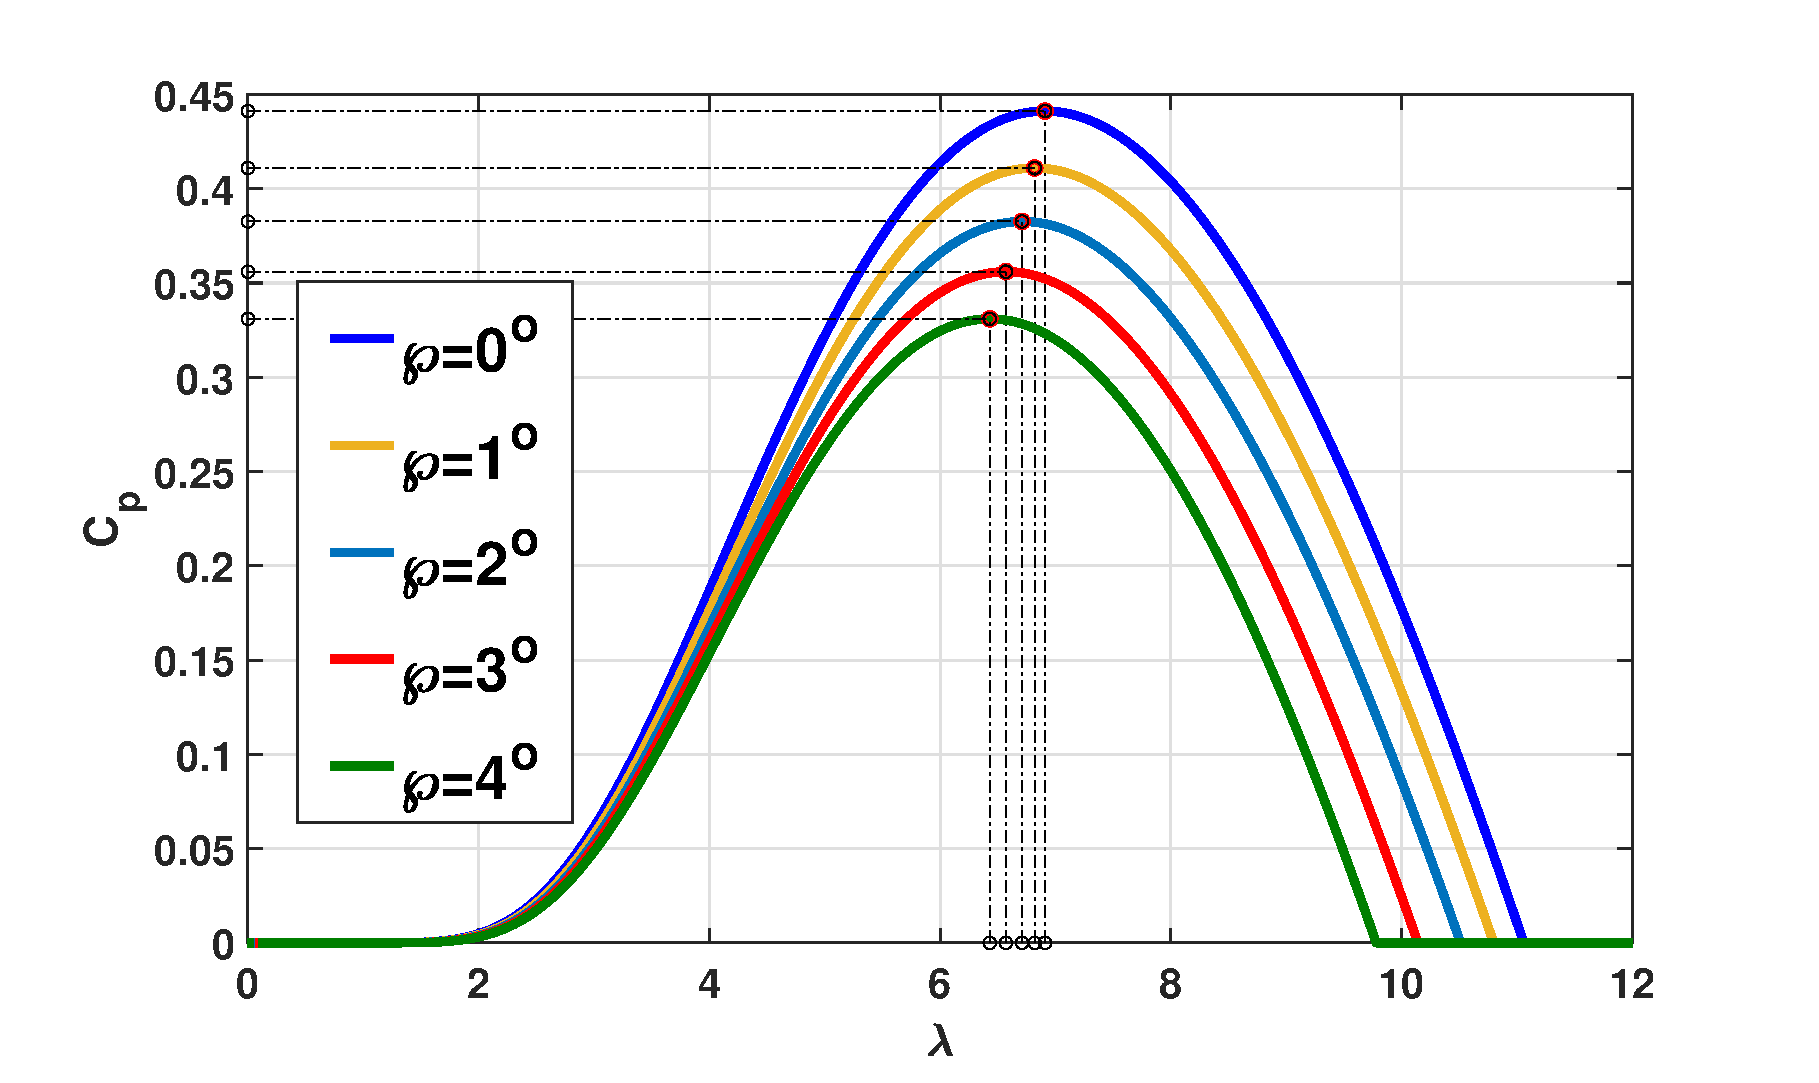
\includegraphics[height=5.8cm,width=11.5cm]{cp.eps}\\
\caption{$\mathrm{C}_{P}$ and $\lambda$ relationship of the PMSG-based WT for varying pitch angle $\wp$ in \eqref{CCP}}\label{CP}
\end{figure}
In addition, Fig. \ref{CP} shows the relationship between $\lambda$ and $\mathcal{C}_P\big( {\lambda},\varphi \big)$. From Fig. \ref{CP}, it can be observe that the power coefficient of $\mathcal{C}_P\big( {\lambda},\varphi \big)$ reach its maximum value $\big(\mathcal{C}_{P\max}\big)$ of $0.441$ only with a certain $\lambda$ value $\mathfrak{\lambda}_{opt}$ of $6.91$, holds the pitch angle $\wp$ of $0$. Therefore, the maximum mechanical torque extracted from the turbine can be expressed as follows:
\begin{eqnarray}
\mathrm{T}_{M}(t)=\frac{{P}_{aero}(t)}{\mathbb{V}_{s}}= 0.5 \upsilon\pi  \mathbb{R}^3 \mathcal{C}_{P\max}\frac{\mathbb{V}^2_{s}}{\lambda(t)}.\label{1}
\end{eqnarray}
Next, the maximum aerodynamic power harnessed from the wind can be represented as follows:
\begin{eqnarray*}
{P}_{aero}(t)= 0.5 \upsilon\pi  \mathbb{R}^2 \mathcal{C}_{P\max}\Big( \frac{\mathbb{R}\omega_{g-opt}(t)}{\lambda_{opt}} \Big)^3,
\end{eqnarray*}
where $\omega_{g-opt}(t)$ is the optimal reference of $\omega_{g}(t)$.
\subsection{{Modeling of PMSG}}
{Let us consider the dynamic model of nonlinear PMSG-based WTS as follows \cite{PMSG2,vel1,sub1}:}
\begin{align}
\begin{cases}\label{2}
\mathrm{L}_{\alpha}\frac{di_{\alpha}(t) }{dt}&=\varpi_e(t) \mathrm{L}_{\beta} i_{\beta}(t)
-\mathrm{R}_si_{\alpha}(t)+\mathrm{V}_{\alpha}(t)\\
\mathrm{L}_{\beta}\frac{di_{\beta} (t)}{dt} &= -\varpi_e(t) \mathrm{L}_{\alpha} i_{\alpha}(t)
-\mathrm{R}_s i_{\beta}(t)
-\varpi_e(t) \phi_{mag}+\mathrm{V}_{\beta}(t),
\end{cases}
\end{align}
where $\varpi_e(t)=\varrho_n \omega_g(t)$ denotes the rotor speed; $\varrho_n$ stand for the  number of pole pairs; $\phi_{mag}$ represents the permanent magnetic flux. $\mathrm{R}_s$ is the stator resistance; $\big(i_{\alpha}(t),i_{\beta}(t)\big)$ and $\big(\mathrm{V}_{\alpha}(t),V_{\beta}(t)\big)$ are the stator currents, and stator voltages in $\alpha-\beta$ reference frame, respectively; $\big(\mathrm{L}_{\alpha},\mathrm{L}_{\beta}\big)$ indicate the stator inductances of the generator in $\alpha-\beta$ reference frame . In this study, we consider the salient pole PMSG system, that is, the $\alpha-\beta$ axis inductances of the generator are equal, that is $\big(\mathrm{L}_{\alpha}=\mathrm{L}_{\beta}=\mathrm{L}\big)$.
Next, the electromagnetic torque can be extracted from the following equation:
\begin{eqnarray*}
\mathrm{T}_{E}&=&1.5\varrho_n\big[ \big(\mathrm{L}_{\alpha}-\mathrm{L}_{\beta}\big)i_{\alpha}(t)i_{\beta}(t)+\phi_{mag}i_{\beta}(t) \big]
\end{eqnarray*}
By substituting $\mathrm{L}_{\alpha}=\mathrm{L}_{\beta}$, we have
$
\mathrm{T}_{E}=1.5\varrho_n\phi_{mag}i_{\beta}(t).
$
The mechanical speed of the PMSG can be described as follows:
\begin{eqnarray}
\mathrm{J}\frac{d\omega_g(t)}{dt}+\Lambda \omega_g(t)&=\mathrm{T}_{E}-\mathrm{T}_{M},\label{4}
\end{eqnarray}
here $\Lambda$ represent the viscous damping coefficient and $\mathrm{J}$ means the moment of inertia.
From \eqref{1}-\eqref{4}, the comprehensive nonlinear dynamic model of PMSG-based WTS can be articulated
as follows:
\begin{eqnarray}
\begin{cases}
\dot{x}(t)=\mathrm{A}\big( \omega_g(t) \big)x(t)+\mathrm{B} u(t)\\
y(t)=\mathrm{C}x(t),\label{5}
\end{cases}
\end{eqnarray}
where $x(t)=\big[\omega_g(t)\;\; i_{\beta}(t)\;\;i_{\alpha}(t)\big]^T=\big[x_1(t)\; x_2(t)\;x_3(t)\big]^T$ stands for the state variables, $y(t)$ denotes the measured output vector, $u(t)=\big[ \mathrm{V}_{\beta}(t)\;\;\mathrm{V}_{\alpha}(t) \big]$, and
\begin{align*}
\mathrm{A}\big( \omega_g(t) \big)&=
\begin{bmatrix}
-\frac{\Lambda+\mathrm{T}_0 \omega_g(t) }{\mathrm{J}}  &  \frac{1.5\varrho_n \phi_{mag}}{\mathrm{J}}& 0\\
\frac{-\varrho_n \phi_{mag} }{\mathrm{L}}&  \frac{-\mathrm{R}_s}{\mathrm{L}}& -\varrho_n  \omega_g(t)\\
0 & \varrho_n  \omega_g(t)& -\frac{\mathrm{R}_s}{\mathrm{L}}
\end{bmatrix},
\mathrm{B}=
\begin{bmatrix}
0&0\\
\frac{1}{\mathrm{L}}&0\\
0&\frac{1}{\mathrm{L}}
\end{bmatrix},\\
\mathrm{C}&=
\begin{bmatrix}
1&0&0
\end{bmatrix},\mathrm{T}_0=\frac{0.5\upsilon\mathcal{C}_{P\max}  \mathbb{R}^5}{\lambda_{opt}^3}.
\end{align*}
{Given the description above, it is crucial to remember that the defined PMSG-based wind turbine model is nonlinear due to the product of the state variable $\omega_g(t)$. Accordingly, based on the Takagi-Sugeno fuzzy modeling technique, the Takagi-Sugeno fuzzy modeling of PMSG-based WTS \eqref{5} is presented in the following subsection.}
\subsection{{Takagi-Sugeno Modeling of PMSG-based WTS}}
In the framework of introducing {Takagi-Sugeno} fuzzy models to approximate the nonlinearity in PMSG-based WTS \eqref{5}, the premise variable is selected as $x_1(t)=\omega_g(t)$, and it is time-varying within the ranges
$\omega_g(t)\in[ d_{\min},d_{\max} ]$. Let us take $\omega_g(t)=\gamma_1d_{\min}+\gamma_2d_{\max}$, where $\gamma_1=[d_{\max}-\omega_g(t)]/[d_{\max}-d_{\min}]$ and $\gamma_2=[\omega_g(t)-d_{\min}]/[d_{\max}-d_{\min}]$.
 As a consequence, the nonlinear system \eqref{5} can be represented in the {Takagi-Sugeno} fuzzy system with the following rules:\\
$\textbf{System rule p:}$ {IF} $\omega_g(t)$ is $\gamma_{p}$, {THEN}
\begin{align}\label{6}
\begin{cases}
\dot{x}(t)&=\mathrm{A}_{p}x(t)+\mathrm{B}_{p}u(t),\\
y(t)&=\mathrm{C}_{p}x(t),\;
\end{cases}
\end{align}
where $\gamma_{p}$ is the fuzzy sets for $p$th rule $(p=1,...,s)$, $r=1$ denote the number of premise
variables, while $s=2$ means the number of fuzzy rules, and
\begin{align*}
\mathrm{A}_1&=
\begin{bmatrix}
-\frac{\Lambda+\mathrm{T}_0 d_{\min} }{\mathrm{J}}  &  \frac{1.5\varrho_n \phi_{mag}}{\mathrm{J}}& 0\\
\frac{-\varrho_n \phi_{mag} }{\mathrm{L}}&  \frac{-\mathrm{R}_s}{\mathrm{L}}& -\varrho_n  d_{\min}\\
0 & \varrho_n  d_{\min}& -\frac{\mathrm{R}_s}{\mathrm{L}}
\end{bmatrix},\;
\mathrm{A}_2=
\begin{bmatrix}
-\frac{\Lambda+\mathrm{T}_0 d_{\max} }{\mathrm{J}}  &  \frac{1.5\varrho_n \phi_{mag}}{\mathrm{J}}& 0\\
\frac{-\varrho_n \phi_{mag} }{\mathrm{L}}&  \frac{-\mathrm{R}_s}{\mathrm{L}}& -\varrho_n  d_{\max}\\
0 & \varrho_n  d_{\max}& -\frac{\mathrm{R}_s}{\mathrm{L}}
\end{bmatrix},\\
\mathrm{B}_1&=\mathrm{B}_2=
\begin{bmatrix}
0&\frac{1}{\mathrm{L}}&0\\
0&0&\frac{1}{\mathrm{L}}
\end{bmatrix}^T,\;
\mathrm{C}_1=\mathrm{C}_2=\big[1\;\;0\;\;0  \big].
\end{align*}
According to a singleton fuzzifier framework, the system \eqref{5} can be expressed as follows:
\begin{align}\label{7}
\begin{cases}
\dot{x}(t)&=\sum^{2}_{p=1}\zeta_p\big( \omega_g(t) \big)\big\{\mathrm{A}_{p}x(t)+\mathrm{B}_{p}u(t)\big\},\\
y(t)&=\sum^{2}_{p=1}\zeta_p\big( \omega_g(t) \big)\mathrm{C}_{p}x(t),\;
\end{cases}
\end{align}
with
$
0\leq\zeta_p(\omega_g(t))=\frac{\gamma_p}{\sum^2_{r=1}\gamma_r}\leq 1,\;\sum^2_{p=1}\gamma_p(\omega_g(t))=1.
$
\subsection{FSDO design}
Suppose the system state variable \eqref{7} is immeasurable at all sampling sequence $t_\kappa$, then the fuzzy state observer for model \eqref{6} should be designed to estimate the states $x(t)$ of system \eqref{7}. {Therefore, the FSDO will be designed to deal with the state estimation of the nonlinear model \eqref{5} based on the fuzzy model \eqref{7}. Inspired by \cite{sub1,obs0,obs1}, the IF-THEN rules of FSDO are given as follows:}\\
$\textbf{Observer rule q:}$ {IF} $\hat{\omega}_g(t)$ is $\hat{\gamma}_{q}$, {THEN}
\begin{align}\label{9a}
\begin{cases}
\dot{\hat{x}}(t)&=\mathrm{A}_{q}\hat{x}(t)+\mathrm{B}_{q}u(t)+\mathrm{H}_q\big(\bar{y}(t) -\hat{y}(t_\kappa) \big)\\
\hat{y}(t)&=\mathrm{C}_{q}\hat{x}(t),\;
\end{cases}
\end{align}
where $\hat{x}(t)$ denote the state estimated by the observer; $\hat{\omega}_g(t)$ and $\hat{\gamma}_{q}$ are the premise variable and fuzzy sets, respectively; $\mathrm{H}_q$ signifies the observer gain matrices to be calculated; $\hat{y}(t_\kappa)$ denotes the outputs of sampled-data fuzzy observer and $\bar{y}(t)=y(t_\kappa)$ stands for the measured sampling output signal. Wherewith, the overall dynamics of the fuzzy observer can be expressed as below:
\begin{align}\label{9}
\begin{cases}
\dot{\hat{x}}(t)&=\sum^{2}_{q=1}\mu_q\big( \hat{\omega}_g(t) \big)\big\{\mathrm{A}_{q}\hat{x}(t)+\mathrm{B}_{q}u(t)
+\mathrm{H}_q\big(\bar{y}(t) -\hat{y}(t_\kappa) \big)\big\},\\
\hat{y}(t)&=\sum^{2}_{q=1}\mu_p\big( \hat{\omega}_g(t) \big)\mathrm{C}_{q}\hat{x}(t),
\end{cases}
\end{align}
where
$
0\leq\mu_p(\hat{\omega}_g(t))=\frac{\hat{\gamma}_p}{\sum^2_{r=1}\hat{\gamma}_r}\leq 1,\;\sum^2_{p=1}\hat{\gamma}_p(\hat{\omega}_g(t))=1.
$
Through the use of $rth$ fuzzy rules, the estimated state $\hat{x}(t)$ can be utilized for the FSDO control design as follows:\\
$\textbf{Controller rule r:}$ {IF} $\hat{\omega}_g(t_\kappa)$ is $\check{\gamma}_{r}$, {THEN}
\begin{align}\label{10}
u(t)&=\mathrm{K}_r \hat{x}(t_\kappa),\;t\in[t_\kappa,t_{\kappa+1}),\;\kappa=0,1,2,...
\end{align}
where $\check{\gamma}_{r}$ are the fuzzy sets, and $\hat{\omega}_g(t_\kappa)$ represent the premise variable; $\mathrm{K}_r$ stands for the controller gain matrices that has to be solved; $t_\kappa$ is the sequence of sampling instants and it satisfying the conditions: $0=t_{0}<t_{1}<t_{2}<...<t_{\kappa-1}< t_\kappa<\cdot\cdot\cdot<\lim_{\kappa\rightarrow \infty}=\infty,\;\kappa=1,2,...,\infty$. Next, the sampling interval is satisfied by
$
0<\tau_m\leq \tau_{\kappa}=t_{\kappa+1}-t_{\kappa}\leq \tau_M,
$
where $\tau_M$ and $\tau_m$ are known the upper and lower bounds of the sampling interval, respectively. Finally, the entire fuzzy controller can be described such that
\begin{align}\label{11}
u(t)&=\sum^{2}_{r=1}\delta_r\big( \hat{\omega}_g(t_\kappa) \big)\mathrm{K}_r \hat{x}(t_\kappa),\;t\in[t_\kappa,t_{\kappa+1}),
\end{align}
where $\delta_r\big( \hat{\omega}_g(t_\kappa) \big)$ represent the membership functions of the designed controller. For brevity, in what follows, this study defines $\zeta_p\big( \omega_g(t) \big)=\zeta_p$, $\mu_q\big( \hat{\omega}_g(t) \big)=\mu_q$, and $\delta_r\big( \hat{\omega}_g(t_\kappa) \big)=\delta_r$.
Then, the overall schematic representation is displayed in Fig. \ref{WTS2}.
\vspace{-0.2cm}
\begin{figure}[h]
\centering
% Graphic for TeX using PGF
% Title: E:\REFERENCES\My papers\paper-7\Dia\control.dia
% Creator: Dia v0.97.2
% CreationDate: Wed Dec 14 19:17:28 2022
% For: PRATAP
% \usepackage{tikz}
% The following commands are not supported in PSTricks at present
% We define them conditionally, so when they are implemented,
% this pgf file will use them.
\ifx\du\undefined
  \newlength{\du}
\fi
\setlength{\du}{2.2\unitlength}
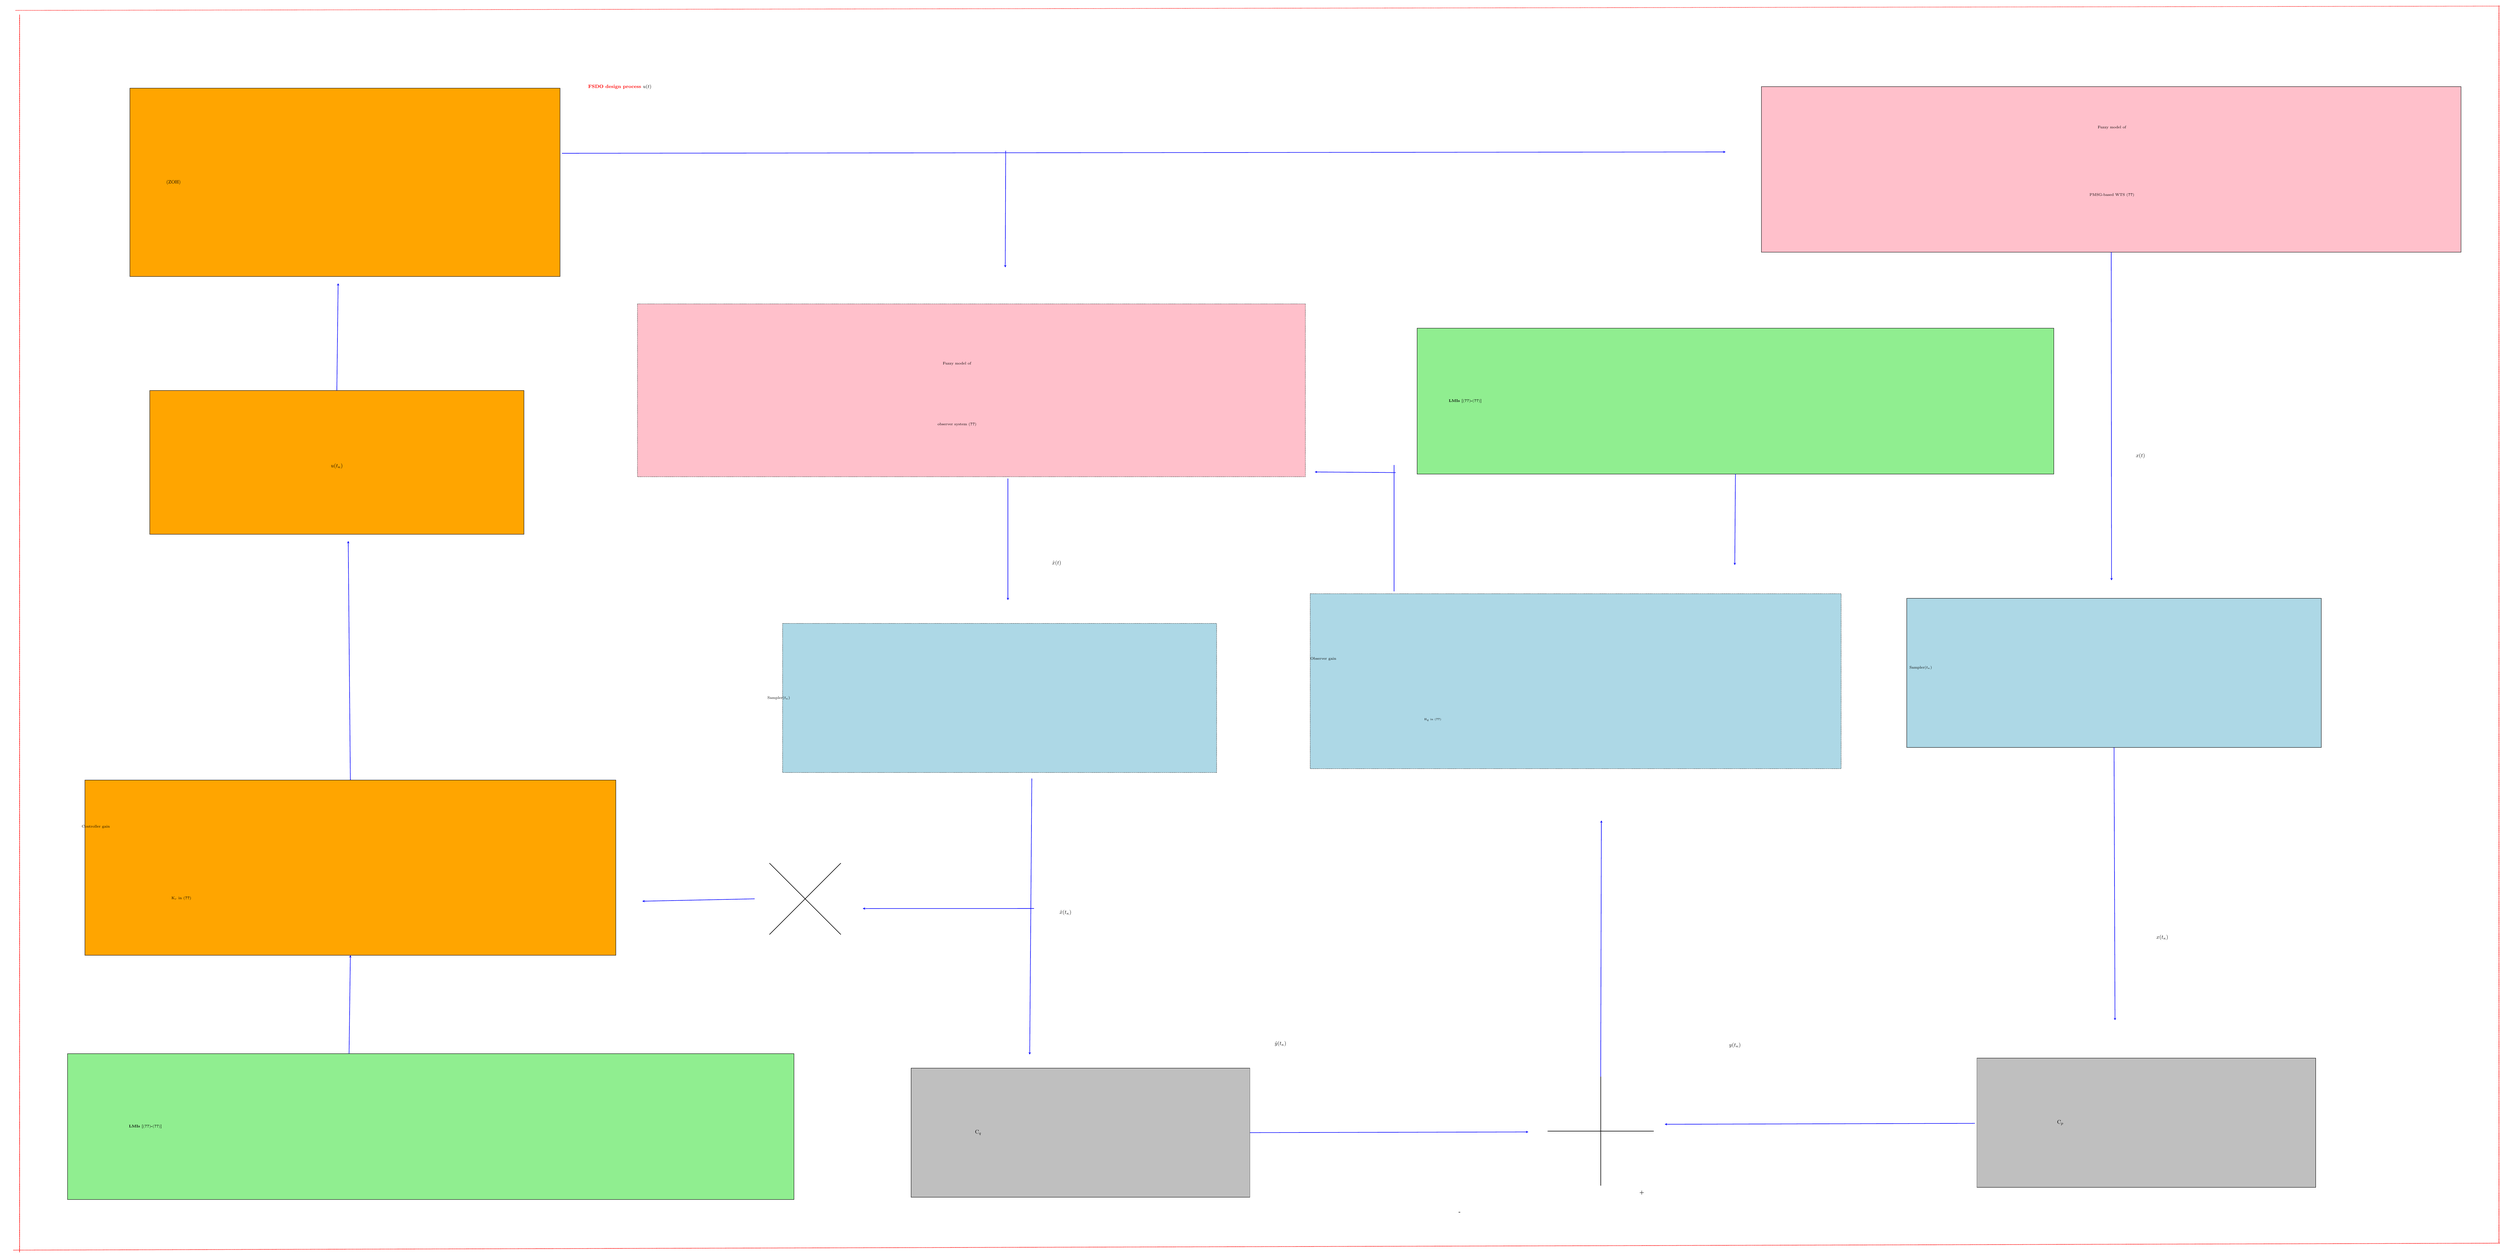
\begin{tikzpicture}
\pgftransformxscale{1.000000}
\pgftransformyscale{-1.000000}
\definecolor{dialinecolor}{rgb}{0.000000, 0.000000, 0.000000}
\pgfsetstrokecolor{dialinecolor}
\definecolor{dialinecolor}{rgb}{1.000000, 1.000000, 1.000000}
\pgfsetfillcolor{dialinecolor}
\definecolor{dialinecolor}{rgb}{1.000000, 0.752941, 0.796078}
\pgfsetfillcolor{dialinecolor}
\fill (62.380000\du,-16.066667\du)--(62.380000\du,-5.166667\du)--(108.420449\du,-5.166667\du)--(108.420449\du,-16.066667\du)--cycle;
\pgfsetlinewidth{0.700000\du}
\pgfsetdash{}{0pt}
\pgfsetdash{}{0pt}
\pgfsetmiterjoin
\definecolor{dialinecolor}{rgb}{0.000000, 0.000000, 0.000000}
\pgfsetstrokecolor{dialinecolor}
\draw (62.380000\du,-16.066667\du)--(62.380000\du,-5.166667\du)--(108.420449\du,-5.166667\du)--(108.420449\du,-16.066667\du)--cycle;
% setfont left to latex
\definecolor{dialinecolor}{rgb}{0.000000, 0.000000, 0.000000}
\pgfsetstrokecolor{dialinecolor}
\node at (85.400225\du,-13.376667\du){\scriptsize{ Fuzzy model of}};
\node at (85.400225\du,-8.929376667\du){\scriptsize{ PMSG-based WTS \eqref{7}}};
\pgfsetlinewidth{1.000000\du}
\pgfsetdash{}{0pt}
\pgfsetdash{}{0pt}
\pgfsetbuttcap
{
\definecolor{dialinecolor}{rgb}{0.000000, 0.000000, 1.000000}
\pgfsetfillcolor{dialinecolor}
% was here!!!
\pgfsetarrowsend{stealth}
\definecolor{dialinecolor}{rgb}{0.000000, 0.000000, 1.000000}
\pgfsetstrokecolor{dialinecolor}
\draw (85.585225\du,27.433333\du)--(85.648180\du,45.384509\du);
}
\definecolor{dialinecolor}{rgb}{0.678431, 0.847059, 0.901961}
\pgfsetfillcolor{dialinecolor}
\fill (71.950000\du,17.620000\du)--(71.950000\du,27.433333\du)--(99.220449\du,27.433333\du)--(99.220449\du,17.620000\du)--cycle;
\pgfsetlinewidth{0.700000\du}
\pgfsetdash{}{0pt}
\pgfsetdash{}{0pt}
\pgfsetmiterjoin
\definecolor{dialinecolor}{rgb}{0.000000, 0.000000, 0.000000}
\pgfsetstrokecolor{dialinecolor}
\draw (71.950000\du,17.620000\du)--(71.950000\du,27.433333\du)--(99.220449\du,27.433333\du)--(99.220449\du,17.620000\du)--cycle;
% setfont left to latex
\definecolor{dialinecolor}{rgb}{0.000000, 0.000000, 0.000000}
\pgfsetstrokecolor{dialinecolor}
\node at (85.585225\du,22.766667\du){};
\pgfsetlinewidth{1.000000\du}
\pgfsetdash{}{0pt}
\pgfsetdash{}{0pt}
\pgfsetbuttcap
{
\definecolor{dialinecolor}{rgb}{0.000000, 0.000000, 1.000000}
\pgfsetfillcolor{dialinecolor}
% was here!!!
\pgfsetarrowsend{stealth}
\definecolor{dialinecolor}{rgb}{0.000000, 0.000000, 1.000000}
\pgfsetstrokecolor{dialinecolor}
\draw (85.400225\du,-5.166667\du)--(85.420449\du,16.433333\du);
}
\definecolor{dialinecolor}{rgb}{0.678431, 0.847059, 0.901961}
\pgfsetfillcolor{dialinecolor}
\fill (32.690449\du,17.313333\du)--(32.690449\du,28.833333\du)--(67.620449\du,28.833333\du)--(67.620449\du,17.313333\du)--cycle;
\pgfsetlinewidth{0.700000\du}
\pgfsetdash{{1.000000\du}{1.000000\du}}{0\du}
\pgfsetdash{{1.000000\du}{1.000000\du}}{0\du}
\pgfsetmiterjoin
\definecolor{dialinecolor}{rgb}{0.000000, 0.000000, 0.000000}
\pgfsetstrokecolor{dialinecolor}
\draw (32.690449\du,17.313333\du)--(32.690449\du,28.833333\du)--(67.620449\du,28.833333\du)--(67.620449\du,17.313333\du)--cycle;
% setfont left to latex
\definecolor{dialinecolor}{rgb}{0.000000, 0.000000, 0.000000}
\pgfsetstrokecolor{dialinecolor}
\node at (50.155449\du,23.313333\du){};
\pgfsetlinewidth{1.000000\du}
\pgfsetdash{}{0pt}
\pgfsetdash{}{0pt}
\pgfsetbuttcap
{
\definecolor{dialinecolor}{rgb}{0.000000, 0.000000, 1.000000}
\pgfsetfillcolor{dialinecolor}
% was here!!!
\pgfsetarrowsend{stealth}
\definecolor{dialinecolor}{rgb}{0.000000, 0.000000, 1.000000}
\pgfsetstrokecolor{dialinecolor}
\draw (76.430000\du,52.171667\du)--(56.020449\du,52.233333\du);
}
\pgfsetlinewidth{1.000000\du}
\pgfsetdash{}{0pt}
\pgfsetdash{}{0pt}
\pgfsetbuttcap
\pgfsetmiterjoin
\pgfsetbuttcap
\pgfsetmiterjoin
\pgfsetdash{}{0pt}
\definecolor{dialinecolor}{rgb}{1.000000, 1.000000, 1.000000}
\pgfsetfillcolor{dialinecolor}
\pgfpathellipse{\pgfpoint{51.803971\du}{52.685981\du}}{\pgfpoint{3.491029\du}{0\du}}{\pgfpoint{0\du}{3.587973\du}}
\pgfusepath{fill}
\definecolor{dialinecolor}{rgb}{0.000000, 0.000000, 0.000000}
\pgfsetstrokecolor{dialinecolor}
\pgfpathellipse{\pgfpoint{51.803971\du}{52.685981\du}}{\pgfpoint{3.491029\du}{0\du}}{\pgfpoint{0\du}{3.587973\du}}
\pgfusepath{stroke}
\pgfsetbuttcap
\pgfsetmiterjoin
\pgfsetdash{}{0pt}
\definecolor{dialinecolor}{rgb}{0.000000, 0.000000, 0.000000}
\pgfsetstrokecolor{dialinecolor}
\draw (51.803971\du,49.098009\du)--(51.803971\du,56.273954\du);
\pgfsetbuttcap
\pgfsetmiterjoin
\pgfsetdash{}{0pt}
\definecolor{dialinecolor}{rgb}{0.000000, 0.000000, 0.000000}
\pgfsetstrokecolor{dialinecolor}
\draw (48.312942\du,52.685981\du)--(55.295000\du,52.685981\du);
\pgfsetlinewidth{1.000000\du}
\pgfsetdash{}{0pt}
\pgfsetdash{}{0pt}
\pgfsetbuttcap
{
\definecolor{dialinecolor}{rgb}{0.000000, 0.000000, 1.000000}
\pgfsetfillcolor{dialinecolor}
% was here!!!
\pgfsetarrowsend{stealth}
\definecolor{dialinecolor}{rgb}{0.000000, 0.000000, 1.000000}
\pgfsetstrokecolor{dialinecolor}
\draw (28.720449\du,52.783333\du)--(47.040150\du,52.738420\du);
}
\pgfsetlinewidth{1.000000\du}
\pgfsetdash{}{0pt}
\pgfsetdash{}{0pt}
\pgfsetbuttcap
{
\definecolor{dialinecolor}{rgb}{0.000000, 0.000000, 1.000000}
\pgfsetfillcolor{dialinecolor}
% was here!!!
\definecolor{dialinecolor}{rgb}{0.000000, 0.000000, 1.000000}
\pgfsetstrokecolor{dialinecolor}
\draw (38.210449\du,17.153333\du)--(38.210449\du,8.833333\du);
}
\pgfsetlinewidth{1.000000\du}
\pgfsetdash{}{0pt}
\pgfsetdash{}{0pt}
\pgfsetbuttcap
{
\definecolor{dialinecolor}{rgb}{0.000000, 0.000000, 1.000000}
\pgfsetfillcolor{dialinecolor}
% was here!!!
\pgfsetarrowsend{stealth}
\definecolor{dialinecolor}{rgb}{0.000000, 0.000000, 1.000000}
\pgfsetstrokecolor{dialinecolor}
\draw (38.309028\du,9.337597\du)--(32.991377\du,9.297597\du);
}
\pgfsetlinewidth{1.000000\du}
\pgfsetdash{}{0pt}
\pgfsetdash{}{0pt}
\pgfsetbuttcap
{
\definecolor{dialinecolor}{rgb}{0.000000, 0.000000, 1.000000}
\pgfsetfillcolor{dialinecolor}
% was here!!!
\pgfsetarrowsend{stealth}
\definecolor{dialinecolor}{rgb}{0.000000, 0.000000, 1.000000}
\pgfsetstrokecolor{dialinecolor}
\draw (12.796185\du,9.733333\du)--(12.796185\du,17.733333\du);
}
\pgfsetlinewidth{1.000000\du}
\pgfsetdash{}{0pt}
\pgfsetdash{}{0pt}
\pgfsetbuttcap
{
\definecolor{dialinecolor}{rgb}{0.000000, 0.000000, 1.000000}
\pgfsetfillcolor{dialinecolor}
% was here!!!
\pgfsetarrowsend{stealth}
\definecolor{dialinecolor}{rgb}{0.000000, 0.000000, 1.000000}
\pgfsetstrokecolor{dialinecolor}
\draw (14.513238\du,38.030599\du)--(3.246471\du,38.034264\du);
}
\pgfsetlinewidth{1.000000\du}
\pgfsetdash{}{0pt}
\pgfsetdash{}{0pt}
\pgfsetbuttcap
\pgfsetmiterjoin
\pgfsetbuttcap
\pgfsetmiterjoin
\pgfsetdash{}{0pt}
\definecolor{dialinecolor}{rgb}{1.000000, 1.000000, 1.000000}
\pgfsetfillcolor{dialinecolor}
\pgfpathellipse{\pgfpoint{-0.548137\du}{37.394203\du}}{\pgfpoint{3.323402\du}{0\du}}{\pgfpoint{0\du}{3.323402\du}}
\pgfusepath{fill}
\definecolor{dialinecolor}{rgb}{0.000000, 0.000000, 0.000000}
\pgfsetstrokecolor{dialinecolor}
\pgfpathellipse{\pgfpoint{-0.548137\du}{37.394203\du}}{\pgfpoint{3.323402\du}{0\du}}{\pgfpoint{0\du}{3.323402\du}}
\pgfusepath{stroke}
\pgfsetbuttcap
\pgfsetmiterjoin
\pgfsetdash{}{0pt}
\definecolor{dialinecolor}{rgb}{0.000000, 0.000000, 0.000000}
\pgfsetstrokecolor{dialinecolor}
\draw (-2.898114\du,35.044225\du)--(1.801841\du,39.744180\du);
\pgfsetbuttcap
\pgfsetmiterjoin
\pgfsetdash{}{0pt}
\definecolor{dialinecolor}{rgb}{0.000000, 0.000000, 0.000000}
\pgfsetstrokecolor{dialinecolor}
\draw (-2.898114\du,39.744180\du)--(1.801841\du,35.044225\du);
\pgfsetlinewidth{1.000000\du}
\pgfsetdash{}{0pt}
\pgfsetdash{}{0pt}
\pgfsetbuttcap
{
\definecolor{dialinecolor}{rgb}{0.000000, 0.000000, 1.000000}
\pgfsetfillcolor{dialinecolor}
% was here!!!
\pgfsetarrowsend{stealth}
\definecolor{dialinecolor}{rgb}{0.000000, 0.000000, 1.000000}
\pgfsetstrokecolor{dialinecolor}
\draw (-30.474551\du,29.583333\du)--(-30.614900\du,13.840000\du);
}
\definecolor{dialinecolor}{rgb}{1.000000, 0.647059, 0.000000}
\pgfsetfillcolor{dialinecolor}
\fill (-43.679551\du,3.933333\du)--(-43.679551\du,13.393333\du)--(-19.049551\du,13.393333\du)--(-19.049551\du,3.933333\du)--cycle;
\pgfsetlinewidth{0.700000\du}
\pgfsetdash{}{0pt}
\pgfsetdash{}{0pt}
\pgfsetmiterjoin
\definecolor{dialinecolor}{rgb}{0.000000, 0.000000, 0.000000}
\pgfsetstrokecolor{dialinecolor}
\draw (-43.679551\du,3.933333\du)--(-43.679551\du,13.393333\du)--(-19.049551\du,13.393333\du)--(-19.049551\du,3.933333\du)--cycle;
% setfont left to latex
\definecolor{dialinecolor}{rgb}{0.000000, 0.000000, 0.000000}
\pgfsetstrokecolor{dialinecolor}
\node at (-31.364551\du,8.903333\du){$u(t_\kappa)$};
\pgfsetlinewidth{1.000000\du}
\pgfsetdash{}{0pt}
\pgfsetdash{}{0pt}
\pgfsetbuttcap
{
\definecolor{dialinecolor}{rgb}{0.000000, 0.000000, 1.000000}
\pgfsetfillcolor{dialinecolor}
% was here!!!
\pgfsetarrowsend{stealth}
\definecolor{dialinecolor}{rgb}{0.000000, 0.000000, 1.000000}
\pgfsetstrokecolor{dialinecolor}
\draw (-16.549551\du,-11.678333\du)--(60.020449\du,-11.766667\du);
}
\definecolor{dialinecolor}{rgb}{1.000000, 0.647059, 0.000000}
\pgfsetfillcolor{dialinecolor}
\fill (-44.979551\du,-15.966667\du)--(-44.979551\du,-3.566667\du)--(-16.679551\du,-3.566667\du)--(-16.679551\du,-15.966667\du)--cycle;
\pgfsetlinewidth{0.700000\du}
\pgfsetdash{}{0pt}
\pgfsetdash{}{0pt}
\pgfsetmiterjoin
\definecolor{dialinecolor}{rgb}{0.000000, 0.000000, 0.000000}
\pgfsetstrokecolor{dialinecolor}
\draw (-44.979551\du,-15.966667\du)--(-44.979551\du,-3.566667\du)--(-16.679551\du,-3.566667\du)--(-16.679551\du,-15.966667\du)--cycle;
% setfont left to latex
\definecolor{dialinecolor}{rgb}{0.000000, 0.000000, 0.000000}
\pgfsetstrokecolor{dialinecolor}
\node at (-30.829551\du,-9.526667\du){};
\pgfsetlinewidth{1.000000\du}
\pgfsetdash{}{0pt}
\pgfsetdash{}{0pt}
\pgfsetbuttcap
{
\definecolor{dialinecolor}{rgb}{0.000000, 0.000000, 1.000000}
\pgfsetfillcolor{dialinecolor}
% was here!!!
\pgfsetarrowsend{stealth}
\definecolor{dialinecolor}{rgb}{0.000000, 0.000000, 1.000000}
\pgfsetstrokecolor{dialinecolor}
\draw (-31.364551\du,3.933333\du)--(-31.279284\du,-3.122789\du);
}
\pgfsetlinewidth{1.000000\du}
\pgfsetdash{}{0pt}
\pgfsetdash{}{0pt}
\pgfsetbuttcap
{
\definecolor{dialinecolor}{rgb}{0.000000, 0.000000, 1.000000}
\pgfsetfillcolor{dialinecolor}
% was here!!!
\pgfsetarrowsend{stealth}
\definecolor{dialinecolor}{rgb}{0.000000, 0.000000, 1.000000}
\pgfsetstrokecolor{dialinecolor}
\draw (12.650449\du,-11.846667\du)--(12.620449\du,-4.166667\du);
}
% setfont left to latex
\definecolor{dialinecolor}{rgb}{0.000000, 0.000000, 0.000000}
\pgfsetstrokecolor{dialinecolor}
%\node[anchor=west] at (-45.829551\du,-12.766667\du){\small{ Zero order hold}};
\node[anchor=west] at (-42.829551\du,-9.766667\du){\small{ (ZOH)}};
% setfont left to latex
\definecolor{dialinecolor}{rgb}{0.000000, 0.000000, 0.000000}
\pgfsetstrokecolor{dialinecolor}
\node[anchor=west] at (15.565100\du,15.300000\du){$\hat{x}(t)$};
\node[anchor=west] at (16.0565100\du,38.300000\du){$\hat{x}(t_\kappa)$};
% setfont left to latex
\definecolor{dialinecolor}{rgb}{0.000000, 0.000000, 0.000000}
\pgfsetstrokecolor{dialinecolor}
%\node[anchor=west] at (54.370449\du,32.513333\du){+};
% setfont left to latex
\definecolor{dialinecolor}{rgb}{0.000000, 0.000000, 0.000000}
\pgfsetstrokecolor{dialinecolor}
%\node[anchor=west] at (45.545100\du,32.690000\du){-};
% setfont left to latex
\definecolor{dialinecolor}{rgb}{0.000000, 0.000000, 0.000000}
\pgfsetstrokecolor{dialinecolor}
\node[anchor=west] at (32.565000\du,21.600000\du){\scriptsize{Observer gain}};
\node[anchor=west] at (40.0565000\du,25.600000\du){\tiny{$\mathrm{H}_{q}$ in \eqref{50}}};
% setfont left to latex
\definecolor{dialinecolor}{rgb}{0.000000, 0.000000, 0.000000}
\pgfsetstrokecolor{dialinecolor}
\node[anchor=west] at (71.985225\du,22.176667\du){\scriptsize{Sampler$(t_\kappa)$}};
% setfont left to latex
\definecolor{dialinecolor}{rgb}{0.000000, 0.000000, 0.000000}
\pgfsetstrokecolor{dialinecolor}
\node[anchor=west] at (-14.959698\du,-16.050000\du){\small{\textcolor{red}{\bf FSDO design process }$u(t)$}};
% setfont left to latex
\definecolor{dialinecolor}{rgb}{0.000000, 0.000000, 0.000000}
\pgfsetstrokecolor{dialinecolor}
\node[anchor=west] at (86.890449\du,8.233333\du){$x(t)$};
% setfont left to latex
\definecolor{dialinecolor}{rgb}{0.000000, 0.000000, 0.000000}
\pgfsetstrokecolor{dialinecolor}
\node[anchor=west] at (88.235100\du,39.940000\du){$x(t_\kappa)$};
% setfont left to latex
\definecolor{dialinecolor}{rgb}{0.000000, 0.000000, 0.000000}
\pgfsetstrokecolor{dialinecolor}
\node[anchor=west] at (60.120449\du,47.033333\du){$y(t_\kappa)$};
\pgfsetlinewidth{1.000000\du}
\pgfsetdash{}{0pt}
\pgfsetdash{}{0pt}
\pgfsetbuttcap
{
\definecolor{dialinecolor}{rgb}{0.000000, 0.000000, 1.000000}
\pgfsetfillcolor{dialinecolor}
% was here!!!
\pgfsetarrowsend{stealth}
\definecolor{dialinecolor}{rgb}{0.000000, 0.000000, 1.000000}
\pgfsetstrokecolor{dialinecolor}
\draw (-30.579551\du,49.133333\du)--(-30.474551\du,41.103333\du);
}
\pgfsetlinewidth{0.700000\du}
\pgfsetdash{}{0pt}
\pgfsetdash{}{0pt}
\pgfsetmiterjoin
\definecolor{dialinecolor}{rgb}{0.564706, 0.933333, 0.564706}
\pgfsetfillcolor{dialinecolor}
\fill (39.720449\du,-0.166667\du)--(39.720449\du,9.433333\du)--(81.620449\du,9.433333\du)--(81.620449\du,-0.166667\du)--cycle;
\definecolor{dialinecolor}{rgb}{0.000000, 0.000000, 0.000000}
\pgfsetstrokecolor{dialinecolor}
\draw (39.720449\du,-0.166667\du)--(39.720449\du,9.433333\du)--(81.620449\du,9.433333\du)--(81.620449\du,-0.166667\du)--cycle;
\pgfsetlinewidth{1.000000\du}
\pgfsetdash{}{0pt}
\pgfsetdash{}{0pt}
\pgfsetbuttcap
{
\definecolor{dialinecolor}{rgb}{0.000000, 0.000000, 1.000000}
\pgfsetfillcolor{dialinecolor}
% was here!!!
\pgfsetarrowsend{stealth}
\definecolor{dialinecolor}{rgb}{0.000000, 0.000000, 1.000000}
\pgfsetstrokecolor{dialinecolor}
\draw (60.670449\du,9.433333\du)--(60.627556\du,15.426227\du);
}
% setfont left to latex
\definecolor{dialinecolor}{rgb}{0.000000, 0.000000, 0.000000}
\pgfsetstrokecolor{dialinecolor}
%\node[anchor=west] at (40.485100\du,16.070000\du){\tiny{\bf Observer gain}};
% setfont left to latex
\definecolor{dialinecolor}{rgb}{0.000000, 0.000000, 0.000000}
\pgfsetstrokecolor{dialinecolor}
\node[anchor=west] at (41.670449\du,4.633333\du){\scriptsize{\bf LMIs [\eqref{44}-\eqref{49}]}};
\definecolor{dialinecolor}{rgb}{1.000000, 0.752941, 0.796078}
\pgfsetfillcolor{dialinecolor}
\fill (-11.579551\du,-1.766667\du)--(-11.579551\du,9.613333\du)--(32.372798\du,9.613333\du)--(32.372798\du,-1.766667\du)--cycle;
\pgfsetlinewidth{0.700000\du}
\pgfsetdash{{1.000000\du}{1.000000\du}}{0\du}
\pgfsetdash{{1.000000\du}{1.000000\du}}{0\du}
\pgfsetmiterjoin
\definecolor{dialinecolor}{rgb}{0.000000, 0.000000, 0.000000}
\pgfsetstrokecolor{dialinecolor}
\draw (-11.579551\du,-1.766667\du)--(-11.579551\du,9.613333\du)--(32.372798\du,9.613333\du)--(32.372798\du,-1.766667\du)--cycle;
% setfont left to latex
\definecolor{dialinecolor}{rgb}{0.000000, 0.000000, 0.000000}
\pgfsetstrokecolor{dialinecolor}
\node at (9.396624\du,2.163333\du){\scriptsize{ Fuzzy model of}};
\node at (9.396624\du,6.163333\du){\scriptsize{ observer system \eqref{9}}};
% setfont left to latex
\definecolor{dialinecolor}{rgb}{0.000000, 0.000000, 0.000000}
\pgfsetstrokecolor{dialinecolor}
%\node[anchor=west] at (14.952624\du,20.133333\du){\tiny{\bf Sampler $t_\kappa$}};
\pgfsetlinewidth{1.000000\du}
\pgfsetdash{}{0pt}
\pgfsetdash{}{0pt}
\pgfsetbuttcap
{
\definecolor{dialinecolor}{rgb}{0.000000, 0.000000, 1.000000}
\pgfsetfillcolor{dialinecolor}
% was here!!!
\pgfsetarrowsend{stealth}
\definecolor{dialinecolor}{rgb}{0.000000, 0.000000, 1.000000}
\pgfsetstrokecolor{dialinecolor}
\draw (14.368977\du,29.474755\du)--(14.230395\du,47.647251\du);
}
\pgfsetlinewidth{1.000000\du}
\pgfsetdash{}{0pt}
\pgfsetdash{}{0pt}
\pgfsetbuttcap
{
\definecolor{dialinecolor}{rgb}{0.000000, 0.000000, 1.000000}
\pgfsetfillcolor{dialinecolor}
% was here!!!
\pgfsetarrowsend{stealth}
\definecolor{dialinecolor}{rgb}{0.000000, 0.000000, 1.000000}
\pgfsetstrokecolor{dialinecolor}
\draw (-3.871538\du,37.394203\du)--(-11.262394\du,37.550491\du);
}
\definecolor{dialinecolor}{rgb}{0.749020, 0.749020, 0.749020}
\pgfsetfillcolor{dialinecolor}
\fill (6.420449\du,48.533333\du)--(6.420449\du,57.033333\du)--(28.720449\du,57.033333\du)--(28.720449\du,48.533333\du)--cycle;
\pgfsetlinewidth{0.700000\du}
\pgfsetdash{}{0pt}
\pgfsetdash{}{0pt}
\pgfsetmiterjoin
\definecolor{dialinecolor}{rgb}{0.000000, 0.000000, 0.000000}
\pgfsetstrokecolor{dialinecolor}
\draw (6.420449\du,48.533333\du)--(6.420449\du,57.033333\du)--(28.720449\du,57.033333\du)--(28.720449\du,48.533333\du)--cycle;
% setfont left to latex
\definecolor{dialinecolor}{rgb}{0.000000, 0.000000, 0.000000}
\pgfsetstrokecolor{dialinecolor}
\node at (17.570449\du,53.023333\du){};
% setfont left to latex
\definecolor{dialinecolor}{rgb}{0.000000, 0.000000, 0.000000}
\pgfsetstrokecolor{dialinecolor}
\node[anchor=west] at (10.50570449\du,52.783333\du){$\mathrm{C}_q$};
\definecolor{dialinecolor}{rgb}{0.678431, 0.847059, 0.901961}
\pgfsetfillcolor{dialinecolor}
\fill (-2.032444\du,19.266176\du)--(-2.032444\du,29.079509\du)--(26.534053\du,29.079509\du)--(26.534053\du,19.266176\du)--cycle;
\pgfsetlinewidth{0.700000\du}
\pgfsetdash{{1.000000\du}{1.000000\du}}{0\du}
\pgfsetdash{{1.000000\du}{1.000000\du}}{0\du}
\pgfsetmiterjoin
\definecolor{dialinecolor}{rgb}{0.000000, 0.000000, 0.000000}
\pgfsetstrokecolor{dialinecolor}
\draw (-2.032444\du,19.266176\du)--(-2.032444\du,29.079509\du)--(26.534053\du,29.079509\du)--(26.534053\du,19.266176\du)--cycle;
% setfont left to latex
\definecolor{dialinecolor}{rgb}{0.000000, 0.000000, 0.000000}
\pgfsetstrokecolor{dialinecolor}
\node at (12.250805\du,24.412843\du){};
\pgfsetlinewidth{0.700000\du}
\pgfsetdash{}{0pt}
\pgfsetdash{}{0pt}
\pgfsetmiterjoin
\definecolor{dialinecolor}{rgb}{0.564706, 0.933333, 0.564706}
\pgfsetfillcolor{dialinecolor}
\fill (-49.079551\du,47.583333\du)--(-49.079551\du,57.183333\du)--(-1.279551\du,57.183333\du)--(-1.279551\du,47.583333\du)--cycle;
\definecolor{dialinecolor}{rgb}{0.000000, 0.000000, 0.000000}
\pgfsetstrokecolor{dialinecolor}
\draw (-49.079551\du,47.583333\du)--(-49.079551\du,57.183333\du)--(-1.279551\du,57.183333\du)--(-1.279551\du,47.583333\du)--cycle;
% setfont left to latex
\definecolor{dialinecolor}{rgb}{0.000000, 0.000000, 0.000000}
\pgfsetstrokecolor{dialinecolor}
\node[anchor=west] at (-45.179551\du,52.383333\du){\scriptsize{\bf LMIs [\eqref{44}-\eqref{49}]}};
\definecolor{dialinecolor}{rgb}{1.000000, 0.647059, 0.000000}
\pgfsetfillcolor{dialinecolor}
\fill (-47.939551\du,29.583333\du)--(-47.939551\du,41.103333\du)--(-13.009551\du,41.103333\du)--(-13.009551\du,29.583333\du)--cycle;
\pgfsetlinewidth{0.700000\du}
\pgfsetdash{}{0pt}
\pgfsetdash{}{0pt}
\pgfsetmiterjoin
\definecolor{dialinecolor}{rgb}{0.000000, 0.000000, 0.000000}
\pgfsetstrokecolor{dialinecolor}
\draw (-47.939551\du,29.583333\du)--(-47.939551\du,41.103333\du)--(-13.009551\du,41.103333\du)--(-13.009551\du,29.583333\du)--cycle;
% setfont left to latex
\definecolor{dialinecolor}{rgb}{0.000000, 0.000000, 0.000000}
\pgfsetstrokecolor{dialinecolor}
\node at (-30.474551\du,35.583333\du){};
% setfont left to latex
\definecolor{dialinecolor}{rgb}{0.000000, 0.000000, 0.000000}
\pgfsetstrokecolor{dialinecolor}
\node[anchor=west] at (-48.374551\du,32.643333\du){\scriptsize{ Controller gain }};
\node[anchor=west] at (-42.374551\du,37.3643333\du){\scriptsize{$\mathrm{K}_{r}$ in \eqref{50}}};
\definecolor{dialinecolor}{rgb}{0.749020, 0.749020, 0.749020}
\pgfsetfillcolor{dialinecolor}
\fill (76.560449\du,47.883333\du)--(76.560449\du,56.383333\du)--(98.860449\du,56.383333\du)--(98.860449\du,47.883333\du)--cycle;
\pgfsetlinewidth{0.700000\du}
\pgfsetdash{}{0pt}
\pgfsetdash{}{0pt}
\pgfsetmiterjoin
\definecolor{dialinecolor}{rgb}{0.000000, 0.000000, 0.000000}
\pgfsetstrokecolor{dialinecolor}
\draw (76.560449\du,47.883333\du)--(76.560449\du,56.383333\du)--(98.860449\du,56.383333\du)--(98.860449\du,47.883333\du)--cycle;
% setfont left to latex
\definecolor{dialinecolor}{rgb}{0.000000, 0.000000, 0.000000}
\pgfsetstrokecolor{dialinecolor}
\node at (87.710449\du,52.373333\du){};
% setfont left to latex
\definecolor{dialinecolor}{rgb}{0.000000, 0.000000, 0.000000}
\pgfsetstrokecolor{dialinecolor}
\node[anchor=west] at (81.710449\du,52.133333\du){$\mathrm{C}_p$};
% setfont left to latex
\definecolor{dialinecolor}{rgb}{0.000000, 0.000000, 0.000000}
\pgfsetstrokecolor{dialinecolor}
\node[anchor=west] at (-3.250805\du,24.172843\du){\scriptsize{ Sampler$(t_\kappa)$}};
% setfont left to latex
\definecolor{dialinecolor}{rgb}{0.000000, 0.000000, 0.000000}
\pgfsetstrokecolor{dialinecolor}
\node[anchor=west] at (30.220449\du,46.933333\du){$\hat{y}(t_\kappa)$};
% setfont left to latex
\definecolor{dialinecolor}{rgb}{0.000000, 0.000000, 0.000000}
\pgfsetstrokecolor{dialinecolor}
\node[anchor=west] at (42.320449\du,58.033333\du){\bf -};
% setfont left to latex
\definecolor{dialinecolor}{rgb}{0.000000, 0.000000, 0.000000}
\pgfsetstrokecolor{dialinecolor}
\node[anchor=west] at (54.220449\du,56.733333\du){\bf +};
\pgfsetlinewidth{1.000000\du}
\pgfsetdash{}{0pt}
\pgfsetdash{}{0pt}
\pgfsetbuttcap
{
\definecolor{dialinecolor}{rgb}{0.000000, 0.000000, 1.000000}
\pgfsetfillcolor{dialinecolor}
% was here!!!
\pgfsetarrowsend{stealth}
\definecolor{dialinecolor}{rgb}{0.000000, 0.000000, 1.000000}
\pgfsetstrokecolor{dialinecolor}
\draw (51.803971\du,49.098009\du)--(51.848476\du,32.232323\du);
}
\pgfsetlinewidth{1.000000\du}
\pgfsetdash{{1.000000\du}{0.400000\du}{0.200000\du}{0.400000\du}}{0cm}
\pgfsetdash{{1.000000\du}{0.400000\du}{0.200000\du}{0.400000\du}}{0cm}
\pgfsetbuttcap
{
\definecolor{dialinecolor}{rgb}{1.000000, 0.000000, 0.000000}
\pgfsetfillcolor{dialinecolor}
% was here!!!
\definecolor{dialinecolor}{rgb}{1.000000, 0.000000, 0.000000}
\pgfsetstrokecolor{dialinecolor}
\draw (-52.520485\du,-21.083528\du)--(111.104024\du,-21.366371\du);
}
\pgfsetlinewidth{1.000000\du}
\pgfsetdash{{1.000000\du}{0.200000\du}{0.200000\du}{0.200000\du}{0.200000\du}{0.200000\du}}{0cm}
\pgfsetdash{{1.000000\du}{0.200000\du}{0.200000\du}{0.200000\du}{0.200000\du}{0.200000\du}}{0cm}
\pgfsetbuttcap
{
\definecolor{dialinecolor}{rgb}{1.000000, 0.000000, 0.000000}
\pgfsetfillcolor{dialinecolor}
% was here!!!
\definecolor{dialinecolor}{rgb}{1.000000, 0.000000, 0.000000}
\pgfsetstrokecolor{dialinecolor}
\draw (-52.661906\du,60.516594\du)--(111.057244\du,60.059693\du);
}
\pgfsetlinewidth{1.000000\du}
\pgfsetdash{{1.000000\du}{0.200000\du}{0.200000\du}{0.200000\du}{0.200000\du}{0.200000\du}}{0cm}
\pgfsetdash{{1.000000\du}{0.200000\du}{0.200000\du}{0.200000\du}{0.200000\du}{0.200000\du}}{0cm}
\pgfsetbuttcap
{
\definecolor{dialinecolor}{rgb}{1.000000, 0.000000, 0.000000}
\pgfsetfillcolor{dialinecolor}
% was here!!!
\definecolor{dialinecolor}{rgb}{1.000000, 0.000000, 0.000000}
\pgfsetstrokecolor{dialinecolor}
\draw (-52.237642\du,-20.800685\du)--(-52.237642\du,60.658016\du);
}
\pgfsetlinewidth{1.000000\du}
\pgfsetdash{{1.000000\du}{0.200000\du}{0.200000\du}{0.200000\du}{0.200000\du}{0.200000\du}}{0cm}
\pgfsetdash{{1.000000\du}{0.200000\du}{0.200000\du}{0.200000\du}{0.200000\du}{0.200000\du}}{0cm}
\pgfsetbuttcap
{
\definecolor{dialinecolor}{rgb}{1.000000, 0.000000, 0.000000}
\pgfsetfillcolor{dialinecolor}
% was here!!!
\definecolor{dialinecolor}{rgb}{1.000000, 0.000000, 0.000000}
\pgfsetstrokecolor{dialinecolor}
\draw (110.915618\du,-21.399214\du)--(110.915618\du,60.059488\du);
}
\end{tikzpicture}
\caption{\small{Schematic diagram of the proposed controller scheme.}} \label{WTS2}
\end{figure}
\vspace{-0.4cm}
By substituting \eqref{11} into \eqref{7}, then the system \eqref{7} can be reformulated as
\begin{align}\label{12}
\dot{x}(t)&=\sum^{2}_{p=1}\sum^{2}_{r=1}\zeta_p\delta_r\big\{\mathrm{A}_{p}x(t)
+\mathrm{B}_{p}\mathrm{K}_r \hat{x}(t_\kappa)\big\}.
\end{align}
Let us define the estimation error $e(t)=x(t)-\hat{x}(t)$, then the {Takagi-Sugeno} fuzzy observer error systems can be obtained follows:
\begin{eqnarray}\label{13}
\dot{e}(t)&=&\sum^{2}_{p=1}\sum^{2}_{q=1}\sum^{2}_{r=1}\zeta_p\mu_q\delta_r\Big\{\mathrm{A}_{q}e(t)
+\big(\mathrm{B}_{q}-\mathrm{B}_{p}\big)\mathrm{K}_r e(t_\kappa)
-\mathrm{H}_q \mathrm{C}_q e(t_\kappa) + \big(\mathrm{A}_{p}-\mathrm{A}_{q}\big)x(t)\nonumber\\
\quad&&+\big(\mathrm{B}_{p}-\mathrm{B}_{q}\big)\mathrm{K}_r x(t_\kappa)
-\mathrm{H}_q \big(\mathrm{C}_{p}-\mathrm{C}_{q}\big) x(t_\kappa) \Big\}.
\end{eqnarray}
From \eqref{12} and \eqref{13}, we can establish the following augmented fuzzy closed-loop system:
\begin{align}\label{14}
\dot{z}(t)&=\sum^{2}_{p=1}\sum^{2}_{q=1}\sum^{2}_{r=1}\zeta_p\mu_q\delta_r\Big\{\mathrm{\widehat{A}}_{pq}z(t)
+\mathrm{\widehat{B}}_{pq}\mathrm{\widehat{K}}_r z(t_\kappa)
+\mathrm{\widehat{H}}_{pq}\mathrm{F}z(t_\kappa)\Big\},
\end{align}
where
\begin{align*}
z(t)&=\big[ x^T(t)\;\;e^T(t) \big]^T,\;
\mathrm{\widehat{A}}_{pq}=
\begin{bmatrix}
\mathrm{A}_{p}& \mathbf{0}\\
\mathrm{A}_{p}-\mathrm{A}_{q}& \mathrm{A}_{q}
\end{bmatrix},\;
\mathrm{\widehat{B}}_{pq}=
\begin{bmatrix}
\mathrm{B}_{p}& -\mathrm{B}_{p}\\
\big(\mathrm{B}_{p}-\mathrm{B}_{q}\big)& -\big(\mathrm{B}_{p}-\mathrm{B}_{q}\big)
\end{bmatrix},\\
\mathrm{\widehat{H}}_{pq}&=
\begin{bmatrix}
\mathrm{H}_q \big(\mathrm{C}_{q}-\mathrm{C}_{p}\big)\\
-\mathrm{H}_q \mathrm{C}_{q}
\end{bmatrix},\;
\mathrm{\widehat{K}}_r=diag\{\mathrm{{K}}_r,\mathrm{{K}}_r\},\;\mathrm{F}=\big[ \mathrm{I}\;\;\mathrm{I} \big].
\end{align*}
\vspace{-0.4cm}
\begin{remark}
{In general, fuzzy observers can be categorized into two types such as immeasurable premise variables observer and measurable premise variables observer. Compared to the immeasurable premise variables observer, the measurable case is easy to implement and provides a wider feasible region. However, it is not realistic because the membership function of the observer depends on the unavailable information of system state $x(t)$. Unlike the existing results on measurable premise variable case \cite{sara1,vino1,prakash1}, the membership functions grade for the proposed observer in this study does not need to coincide with the considered system and its controller, that is $\zeta_p\big( \omega_g(t) \big)\neq\mu_q\big( \hat{\omega}_g(t) \big)\neq\delta_r\big( \hat{\omega}_g(t_\kappa) \big)$. Meanwhile, if $\zeta_p\big( \omega_g(t) \big)=\mu_q\big( \hat{\omega}_g(t) \big)=\delta_r\big( \hat{\omega}_g(t_\kappa) \big)$, then the designed observer shares the identical structure of membership functions with the system, which indicates that the observer is designed based on the measurable premise variables condition. Also, this measurable premise variable case is ineffective under network environments, at the same time, the unmeasurable premise variable case has provided superior robustness properties than the conventional case \cite{pengc}. Therefore, the designed fuzzy observer in this study is more general and practical. }
\end{remark}
Before ending this subsection, widely used assumption, and some important lemmas are introduced to facilitate the main results.

{Assumption 1:}\cite{obs1} The weighting membership function imply with
$
\big|{\dot{\mu}_q\big( \hat{\omega}_g(t) \big)\big|}\leq \hbar_q,\;q=1,2,
$
where $\hbar_q>0$ are constants.
\begin{remark}
{It should be mentioned that the upper bounds of the fuzzy membership function-related information do not need to be known in real time because the system state during the whole control process is unpredictable, the above limitation cannot be fundamentally eliminated. In this study, the upper bounds of the membership function in this study are a presupposed value with a certain margin, which means the upper bound of $\big|{\dot{\mu}_q\big( \hat{\omega}_g(t) \big)\big|}$ can be restricted to a predefined region. Thus, how to pre-set an accurate value for the upper bounds of the time derivative of the fuzzy membership functions will become the direction of our future research.}
\end{remark}
\vspace{-0.5cm}
\begin{lemma} \cite{lem2} (Singular value decomposition technique $(\mathcal{SVD})$)\label{lem2}
For full rank matrix $i=rank(\mathrm{C})$ with $\mathrm{C}\in \mathbb{R}^{i\times j}$, the $\mathcal{SVD}$ for $\mathrm{C}$ can be defined as $\mathrm{C}=\mathbb{O}\big[ \mathbb{S}\;\;0 \big]\mathbb{V}^T$, here $\mathbb{V.V^T}=\mathrm{I}$ and $\mathbb{O.O}^T=\mathrm{I}$. Let matrices $\mathbb{G}>0$, $\mathbb{G}_1\in \mathbb{R}^{i\times i}$ and $\mathbb{G}_2\in  \mathbb{R}^{j\times j}$, there exists $\mathcal{G}$ such that $\mathrm{C}\mathbb{G}=\mathcal{G}\mathrm{C}$ if and only if the condition
$\mathbb{G}=\mathbb{V}\begin{bmatrix}
\mathbb{G}_1& 0\\
0&\mathbb{G}_2
\end{bmatrix}\mathbb{V^T}$ is satisfied.
\end{lemma}
\begin{lemma}\cite{lem1}\label{lem1}
For any matrix $\mathrm{Y}$ and a scalar $h$, the following inequality holds,
\begin{eqnarray*}
h\big(\mathrm{Y}+\mathrm{Y}^T  \big)\leq h^2 \mathrm{V}+ \mathrm{Y}\mathrm{V}^{-1} \mathrm{Y}^T
\end{eqnarray*}
where $\mathrm{V}>0$ is a positive definite matrix.
\end{lemma}
\vspace{-0.5cm}
\begin{lemma} {(\bf AFBII)}\label{Lemma3}
Let $z(t)$ be a continuously differentiable function on $[\lambda_{1},\lambda_{2}]\rightarrow \mathbb{R}^{2n}$, where $\lambda_{1},\lambda_{2}$ are any scalars with $\lambda_{1}<\lambda_{2}$. For any positive symmetric matrix $\mathrm{Z}\in \mathbb{R}^{4n\times 4n}$ holds the following inequality:
\begin{align}\label{15}
-\int^{\lambda_2}_{\lambda_1}{\omega}^T(\nu)\mathrm{Z}{\omega}(\nu)d\nu
&\leq sym\big[ \xi_1^T \mathrm{X}_1\Delta_1\Re+\xi_1^T\mathrm{X}_2\Delta_2\Re-2\xi_2^T\mathrm{X}_3\Delta_2\Re\big]\nonumber\\
&+\lambda_{12}\Big\{sym[\xi_2^T\mathrm{X}_3\Delta_3\Re]+ \xi_1^T \big[\mathrm{X}_1\;\;\mathrm{X}_2 \big]\mathrm{Z}^{-1}\big[ \mathrm{X}_1\;\;\mathrm{X}_2 \big]^T\xi_1\nonumber\\
&+\frac{\lambda_{12}^2}{3}\xi_2^T\big[ \mathrm{X}_3\;\;0_{gn\times2n} \big]\mathrm{Z}^{-1}\big[ \mathrm{X}_3\;\;0_{gn\times2n} \big]^T\xi_2
 \Big\},
\end{align}
where $\xi_1,\xi_2$ and $\Re$ are any vectors, while $\mathrm{X}_1,\mathrm{X}_2,\mathrm{X}_3$ are any matrices with compatible dimensions, and
\begin{align*}
\Delta_1\Re\;&=z(\lambda_2)-z(\lambda_1),\;
\Delta_2\Re\;=\int^{\lambda_2}_{\lambda_1}z(\nu)d\nu,\;\lambda_{12}=\lambda_2-\lambda_1,\;\\
\Delta_3\Re\;&=z(\lambda_1)+z(\lambda_2),\;
\omega(\nu)=\Big[\dot{z}^T(\nu)\;\;z^T(\nu)\Big]^T.
\end{align*}
$\textbf{Proof.}$ Let us define two polynomial functions and a structured matrix $\mathrm{X}$ such that
\begin{eqnarray*}
\beta_1(\nu)&=&1,\;
\beta_2(\nu)=\frac{2\nu-\lambda_1-\lambda_2}{2},\;
\mathrm{X}=
\begin{bmatrix}
\mathrm{X}_3   &  0_{gn\times 2n}\\
\mathrm{X}_1 &  \mathrm{X}_2
\end{bmatrix}
\end{eqnarray*}
and
$
\varepsilon(\nu)=\big[ \sigma_2\beta_2(\nu)\xi_2^T,\sigma_1\beta_1(\nu)\xi_1^T,\omega^T(\nu)\big]^T,
$
where $\sigma_1$ and $\sigma_2$ are any scalars to be decided. Then, based on the Schur complement and the fact $\mathrm{Z}>0$, the following is natural:
\begin{eqnarray*}
\mathrm{W}=
\begin{bmatrix}
  \mathrm{X}\mathrm{Z}^{-1}\mathrm{X}^T&      \mathrm{X}\\
  \star&         \mathrm{Z}
\end{bmatrix}\geq0.
\end{eqnarray*}
It is easy to see that
\begin{align}\label{16}
\varepsilon^T(\nu)\mathrm{W} \varepsilon(\nu)\geq0.
\end{align}
Integrating the inequality from \eqref{16} over the range of $\nu=\lambda_1$ to $\nu=\lambda_2$ gives
\begin{align}\label{17}
\int^{\lambda_2}_{\lambda_1}\varepsilon^T(\nu)\mathrm{W} \varepsilon(\nu)d\nu
&=\int^{\lambda_2}_{\lambda_1}
\begin{bmatrix}
\sigma_2\beta_2(\nu)\xi_2\\
\sigma_1\beta_1(\nu)\xi_1
\end{bmatrix}^T
\mathrm{X}\mathrm{Z}^{-1}\mathrm{X}^T
\begin{bmatrix}
\sigma_2\beta_2(\nu)\xi_2\\
\sigma_1\beta_1(\nu)\xi_1
\end{bmatrix}
d\nu \nonumber\\
&+2\int^{\lambda_2}_{\lambda_1}
\begin{bmatrix}
\sigma_2\beta_2(\nu)\xi_2\\
\sigma_1\beta_1(\nu)\xi_1
\end{bmatrix}^T
\begin{bmatrix}
\dot{z}(\nu)\\
z(\nu)
\end{bmatrix}
d\nu
+\int^{\lambda_2}_{\lambda_1}{\omega}^T(\nu)\mathrm{Z}{\omega}(\nu)d\nu\nonumber\\
&=\nu^2_1\xi_1^T \big[\mathrm{X}_1\;\;\mathrm{X}_2 \big]\mathrm{Z}^{-1}\big[ \mathrm{X}_1\;\;\mathrm{X}_2 \big]^T\xi_1
\int^{\lambda_2}_{\lambda_1} \beta^2_1(\nu)d\nu\nonumber\\
&+\nu^2_2\xi_2^T\big[ \mathrm{X}_3\;\;0_{gn\times2n} \big]\mathrm{Z}^{-1}\big[ \mathrm{X}_3\;\;0_{gn\times2n} \big]^T\xi_2
\int^{\lambda_2}_{\lambda_1} \beta^2_2(\nu)d\nu\nonumber\\
&+2\sigma_1\xi_1^T\mathrm{X}_1\int^{\lambda_2}_{\lambda_1}\dot{z}(\nu)d\nu
+2\sigma_2\xi_2^T\mathrm{X}_3\int^{\lambda_2}_{\lambda_1}\beta_2(\nu)\dot{z}(\nu)d\nu\nonumber\\
&+2\sigma_1\xi_1^T\mathrm{X}_2\Delta_2\Re
+\int^{\lambda_2}_{\lambda_1}{\omega}^T(\nu)\mathrm{Z}{\omega}(\nu)d\nu\geq0.
\end{align}
Considering the fact that
\begin{align}
\int^{\lambda_2}_{\lambda_1}\beta^2_1(\nu)d\nu&=\lambda_{21},\;
\int^{\lambda_2}_{\lambda_1}\beta^2_2(\nu)d\nu= \frac{\lambda_{12}^3}{12},\label{18}\\
\int^{\lambda_1}_{\lambda_2}\beta_1(\nu)\beta_2(\nu)d\nu&=0,\;
\int^{\lambda_2}_{\lambda_1}\dot{x}(\nu)d\nu=\Delta_1\Re,\label{19}\\
\int^{\lambda_2}_{\lambda_1}\beta_2(\nu)\dot{x}(\nu)d\nu&=-\Delta_2\Re+\frac{\lambda_{12}}{2}\Delta_3\Re.\label{20}
\end{align}
Substituting \eqref{18}-\eqref{20} into \eqref{17}, we have
\begin{align}\label{21}
-\int^{\lambda_2}_{\lambda_1}{\omega}^T(\nu)\mathrm{Z}{\omega}(\nu)d\nu
&\leq sym\Big\{  \sigma_1\xi_1^T\mathrm{X}_1\Delta_1\Re
+\sigma_2\xi_2^T\mathrm{X}_3\big(-\Delta_2\Re+\frac{\lambda_{12}}{2}\Delta_3\Re\big)\nonumber\\
&+ \sigma_1\xi_1^T \mathrm{X}_2\Delta_2\Re\Big\}+\lambda_{12}\Big\{ \nu^2_1\xi_1^T \big[\mathrm{X}_1\;\;\mathrm{X}_2 \big]\mathrm{Z}^{-1}\big[ \mathrm{X}_1\;\;\mathrm{X}_2 \big]^T\xi_1\nonumber\\
&+\frac{\nu^2_2\lambda_{12}^2}{12}\xi_2^T\big[ \mathrm{X}_3\;\;0_{gn\times2n} \big]\mathrm{Z}^{-1}\big[ \mathrm{X}_3\;\;0_{gn\times2n} \big]^T\xi_2
\Big\}.
\end{align}
Letting $\sigma_1=1$ and $\sigma_2=2$, then, rearranging the inequality \eqref{21} yield \eqref{15}. This completes the proof.
\end{lemma}
\vspace{-0.3cm}
${\bf Problem\;1:}$ {The main control objective of this study is to determine $\mathrm{H}_q$ of the FSDO \eqref{9} and $\mathrm{K}_r\;(q,r=1,2)$ of the fuzzy controller \eqref{11} such that the following objectives can be achieved:}
\begin{itemize}
\item[1)] {The augmented fuzzy closed-loop system \eqref{14} is globally asymptotically stable for any initial condition, i.e., $z(t)\rightarrow0$ as $t\rightarrow\infty$.}
\item[2)] {The controller gain and observer gain matrices $\mathrm{K}_r\;(r,q=1,2)$ and $\mathrm{H}_q\;(r,q=1,2)$ are calculated through solvable LMIs to ensure the state estimation of the fuzzy PMSG-based system \eqref{5} by the designed FSDO \eqref{9}.}
\end{itemize}
\vspace{-0.3cm}
\section{Main Results}
In this section, we first present the asymptotic stability condition of augmented fuzzy closed-loop system \eqref{14} with the help of proposed AFBII and suitable DSLLKF. And then, an effective controller algorithm of asynchronous observer and controller gain matrices is designed through the $\mathcal{SVD}$ technique.
Before proceeding to the main results, the following abbreviation are defined: $\theta_1=(t_{k+1}-t)$, $\theta_2=(t-t_{k})$,
$\Pi\big(\lambda_1,\lambda_2,\pi\big)=\int^{\lambda_2}_{\lambda_1}\pi(\nu)d\nu$,
$\nabla_1(t)=\big[ z^T(t),z^T(t_k),\Pi\big(t_k,t,{z}\big) \big]^T$, $\nabla_2(t_k)=\big[ z^T(t_k),z^T(t_{k+1}),\Pi\big(t_k,t_{k+1},{z}\big) \big]^T$,
$\nabla_3(t)=\big[ \dot{z}^T(t),z^T(t) \big]^T$,
$\wp_c=\big[0_{2n\times(c-1)2n}\;\; \mathrm{I}_{2n}\;\;0_{2n\times(6-c)2n}  \big],\;c=1,2,...,6$, and
$\Re(t)=\big[ z^T(t)\;\;\dot{z}^T(t)\\\;z^T(t_k)\;\;z^T(t_{k+1}) \;\;\Pi\big(t_{k},t,{z}\big)\;\;\Pi\big(t,t_{k+1},{z}\big) \big]$.
Next, we are ready to derive the stability condition of augmented fuzzy closed-loop system \eqref{14}.
\begin{Thm}\label{Thm12}
Given that scalars $0<\tau_m<\tau_M$, $\hbar_1,\hbar_2$, {$0<\chi_r< 1$} satisfying {$\delta_r\big(\hat{\omega}_g(t_\kappa)\big)-{\chi}_r\mu_r\big(\hat{\omega}_g(t)\big)\geq 0\;(\chi_r>0)$,} and assuming that gain matrices $\mathrm{K}_i,\;\mathrm{H}_i$ are known, the augmented fuzzy closed-loop system \eqref{14} is asymptotically stable if there exist symmetric matrices $0<\mathrm{P}_i\in  \mathbb{R}^{2n\times 2n},\; 0<\mathrm{Z}_i\in  \mathbb{R}^{4n\times4n}, \; 0<{\mathcal{F}_i}\in  \mathbb{R}^{2n\times 2n},\;\mathrm{Q}_i\in  \mathbb{R}^{2n\times 2n}$, $\mathrm{S}\in  \mathbb{R}^{6n\times 6n},\;\mathrm{U}\in  \mathbb{R}^{2n\times 2n}$, $\Gamma_p\in  \mathbb{R}^{24n\times 24n}$, any matrices $ \mathrm{H}_i\in  \mathbb{R}^{2n\times 6n}$,
$ \mathrm{X}_i\in  \mathbb{R}^{g_1n\times 2n}$, $ \mathrm{X}_3\in  \mathbb{R}^{g_2n\times 2n}$,
$ \mathrm{Y}_i\in  \mathbb{R}^{h_1n\times 2n}$, $ \mathrm{Y}_3\in  \mathbb{R}^{h_2n\times 2n}$, $ \mathrm{N}_j\in  \mathbb{R}^{2n\times 2n}$,
$\mathrm{R}_l\in  \mathbb{R}^{2n\times 2n}\;(i=1,2,\;j=1,2,3,\;l=1,2,3,4,5)$ so as to hold the following inequalities for $\tau_\kappa\in\{ \tau_m,\tau_M \}$:
\begin{align}
&{\chi}_p\big[ \Theta_{pqp,\tau'}\big]_{\tau_\kappa} -{\chi}_p\Gamma_p+ \Gamma_p<0,\label{23}\\
& \big[ \Theta_{pqr,\tau'}\big]_{\tau_\kappa} - \Gamma_p<0,\label{24}\\
&{\chi}_p\big[ \Theta_{rqp,\tau'}\big]_{\tau_\kappa}+{\chi}_r\big[\Theta_{pqr,\tau'}\big]_{\tau_\kappa}
 - {\chi}_p\Gamma_r- {\chi}_r\Gamma_p+\Gamma_p+\Gamma_r<0,\label{28}
\end{align}
where $\;\tau'=a,b,$
\begin{align*}
\big[ \Theta_{pqr,a}\big]_{\tau_\kappa}&=
 \begin{bmatrix}
 \Theta_1^{pqr}+\tau_\kappa\Theta_2& \star&\star&\star&\star\\
 \sqrt{\tau_\kappa}\big[ \mathrm{Y}_1\;\;\mathrm{Y}_2 \big]^T\xi_{21}&-\mathrm{Z}_2&\star&\star&\star\\
 \tau_M \sqrt{\tau_\kappa}\big[ \mathrm{Y}_3\;\;\mathbf{0} \big]^T\xi_{22}&\mathbf{0}&-3\mathrm{Z}_2&\star&\star\\
 (\mathrm{P}_1+\mathrm{U})\wp_1&\mathbf{0}&\mathbf{0}&-{\mathcal{F}}_1&\star\\
 (\mathrm{P}_2+\mathrm{U})\wp_1&\mathbf{0}&\mathbf{0}&\mathbf{0}&-{\mathcal{F}}_2
 \end{bmatrix},\\
\big[ \Theta_{pqr,b}\big]_{\tau_\kappa}&=
 \begin{bmatrix}
 \Theta_1^{pqr}+\tau_\kappa\Theta_3& \star&\star&\star&\star\\
 \sqrt{\tau_\kappa}\big[ \mathrm{X}_1\;\;\mathrm{X}_2 \big]^T\xi_{11}&-\mathrm{Z}_1&\star&\star&\star\\
 \tau_M \sqrt{\tau_\kappa}\big[ \mathrm{X}_3\;\;\mathbf{0} \big]^T\xi_{12}&\mathbf{0}&-3\mathrm{Z}_1&\star&\star\\
 (\mathrm{P}_1+\mathrm{U})\wp_1&\mathbf{0}&\mathbf{0}&-{\mathcal{F}}_1&\star\\
 (\mathrm{P}_2+\mathrm{U})\wp_1&\mathbf{0}&\mathbf{0}&\mathbf{0}&-{\mathcal{F}}_2
 \end{bmatrix},
\end{align*}
with
\begin{eqnarray*}
\Theta_1^{pqr}&=&sym\big\{\wp^T_1\mathrm{P}_q\wp_2+(\wp_3-\wp_1)^T\mathrm{H}_1\Psi_1+\wp^T_1\mathrm{H}_2\Psi_1
-\wp_4^T\mathrm{H}_2\Psi_1+\Xi_0\Xi_{1pqr}+ \xi_{11}^T \mathrm{X}_1(\wp_1-\wp_3)\\
\quad&&+\xi_{11}^T\mathrm{X}_2\wp_5-2\xi_{12}^T\mathrm{X}_3\wp_5+\xi_{21}^T \mathrm{Y}_1(\wp_4-\wp_1)
+\xi_{21}^T\mathrm{Y}_2\wp_6-2\xi_{22}^T\mathrm{Y}_3\wp_6
\big\}-\Psi_2^T\mathrm{R}\Psi_2\\
\quad&&+0.25\wp^T_1\Big[ \sum^{2}_{q=1}\hbar_q^2{\mathcal{F}_q}\Big]\wp_1
+(\wp_3-\wp_1)^T\mathrm{Q}_1(\wp_1-\wp_3)
+(\wp_1-\wp_4)^T\mathrm{Q}_2(\wp_1-\wp_4),\\
\Theta_2&=&sym\big\{ \Psi_2^T\mathrm{R}\Psi_3+\wp_2^T\mathrm{Q}_1(\wp_1-\wp_3)+\wp_2^T\mathrm{H}_1\Psi_1
+\xi_{22}^T\mathrm{Y}_3(\wp_1+\wp_4) \big\}+\Psi_1^T\mathrm{S}\Psi_1+\Psi_4^T\mathrm{Z}_2\Psi_4,\\
\Theta_3&=&sym\big\{ \wp_2^T\mathrm{Q}_2(\wp_1-\wp_4)+\wp_2^T\mathrm{H}_2\Psi_1
+\xi_{12}^T \mathrm{X}_3(\wp_1+\wp_3) \big\}-\Psi_1^T\mathrm{S}\Psi_1+\Psi_4^T\mathrm{Z}_1\Psi_4
\end{eqnarray*}
with $\xi_{11}\in  \mathbb{R}^{g_1n\times 2n},\;\xi_{12}\in  \mathbb{R}^{g_2n\times 2n},\;\xi_{21}\in  \mathbb{R}^{h_1n\times 2n},\;\xi_{22}\in  \mathbb{R}^{h_2n\times 2n}$ may be selected as $\wp_c$ or its part, $\Xi_0=\wp^T_1\mathrm{N}_1+\wp^T_2\mathrm{N}_2+\wp^T_3\mathrm{N}_3$,
$\Xi_{1pqr}=\mathrm{\widehat{A}}_{pq}\wp_1+\mathrm{\widehat{B}}_{pqr}\wp_3+\mathrm{\widehat{H}}_{pq}\mathrm{F}\wp_3-\wp_2$,
$\Psi_1=\big[\wp^T_3,\wp^T_4,(\wp_5+\wp_6) ^T \big]^T$, $\Psi_2=\big[\wp^T_1,\wp^T_3,\wp_5^T \big]^T$, $\Psi_3=\big[\wp^T_2,\mathbf{0},\wp_1^T \big]^T$, $\Psi_4=\big[\wp^T_2,\wp_1^T \big]^T$.
\end{Thm}
\begin{proof}
First, a novel DSLLKF for the augmented closed-loop system \eqref{14} is proposed to derive the main results as a solution to Problem 1. The functional is
\begin{align}\label{22}
\mathrm{V}(t)&=\mathrm{V}_p(t)+\sum^4_{m=1}\mathrm{V}_{lm}(t),\;t_k\leq t<t_{k+1},
\end{align}
where\vspace{-0.3cm}
\begin{align*}
\mathrm{V}_p(t)&=\sum^{2}_{q=1}\mu_q\big( \hat{\omega}_g(t) \big)\big\{z^T(t)\mathrm{P}_qz(t)\big\}\\
\mathrm{V}_{l1}(t)&=\theta_1\Big\{\nabla^T_1(t)\mathrm{R}\nabla_1(t)+\theta_2\nabla^T_2(t_k)\mathrm{S}\nabla_2(t_k)\Big\}\\
\mathrm{V}_{l2}(t)&=\theta_1\Pi^T\big(t_k,t,\dot{z}\big)\Big\{ \mathrm{Q}_1\Pi\big(t_k,t,\dot{z}\big)+2\mathrm{H}_1 \nabla_2(t_k)\Big\}\\
\mathrm{V}_{l3}(t)&=\theta_2\Pi^T\big(t_{k+1},t,\dot{z}\big)\Big\{ \mathrm{Q}_2\Pi\big(t_{k+1},t,\dot{z}\big)+2\mathrm{H}_2 \nabla_2(t_k)\Big\}\\
\mathrm{V}_{l4}(t)&=\theta_1\int^t_{t_k}\nabla^T_3(\nu)\mathrm{Z}_1\nabla_3(\nu)d\nu
-\theta_2\int^{t_{k+1}}_{t}\nabla^T_3(\nu)\mathrm{Z}_2\nabla_3(\nu)d\nu
\end{align*}
with
$\mathrm{R}=
\begin{bmatrix}
\mathrm{R}_{11}  &   \star&  \star\\
2n\mathrm{R}^T_{2}& \mathrm{R}_{22} &  \star\\
\mathrm{R}^T_{3} & \mathrm{R}^T_{4}& \mathrm{R}_{5}+\mathrm{R}^T_{5}
\end{bmatrix},$
$\mathrm{R}_{11}=sym\{m\mathrm{R}_1\}-sym\{n\mathrm{R}_2\},\;
\mathrm{R}_{22}=-sym\{m\mathrm{R}_1\}-sym\{n\mathrm{R}_2\}$, $m$ and $n$ are known constants, $\mathrm{P}_q>0$, $\mathrm{Z}_i>0$, $\mathrm{S}$ and $\mathrm{Q}_i$ are symmetric matrices, $\mathrm{R}$ and $\mathrm{H}_i\;(i=1,2)$ are any matrices with suitable dimensions to be estimated. Further, it can be seen that  $\lim_{t\rightarrow t^+_k}\mathrm{V}_{lf}(t)=\lim_{t\rightarrow t^-_k}\mathrm{V}_{lf}(t)=0\;(f=1,2,3,4)$ in \eqref{22}, {ensuring that $\mathrm{V}(t)$ is positive definite at sampling
instants, while the positive definiteness within the sampling interval is not required.} As a result, we have $\mathrm{V}(t_k)=\lim_{t\rightarrow t^+_k}\mathrm{V}(t)=\lim_{t\rightarrow t^-_k}\mathrm{V}(t)>0$, {and it shows that the proposed DSLLKF \eqref{22} is continuous and satisfies the looped-type functional condition given in \cite{LP-1,LP-2,LP-3}.} Next, taking the time derivative of $\mathrm{V}_p(t)$ along the trajectories of system \eqref{14}, we have
\begin{align}
\mathrm{\dot{V}}_p(t)=2z^T(t)\mathrm{P}(t)\dot{z}(t)
+\sum^{2}_{q=1}\dot{\mu}_q\big( \hat{\omega}_g(t) \big)\big\{z^T(t)\mathrm{P}_qz(t)\big\},\label{29}
\end{align}
where $\mathrm{P}(t)=\sum^{2}_{q=1}\mu_q\big( \hat{\omega}_g(t) \big)\mathrm{P}_q$. Then, based on the fuzzy membership function property, we can obtain
$\sum^{2}_{q=1}\mu_q\big( \hat{\omega}_g(t) \big)=1$ and  $\sum^{2}_{q=1}\dot{\mu}_q\big( \hat{\omega}_g(t) \big)=0$. For any suitable dimension of slack matrix $\mathrm{U}$, we obtain the following zero equation $\sum^{2}_{q=1}\dot{\mu}_q\big( \hat{\omega}_g(t) \big)z^T(t)\mathrm{U}z(t)=0$. As a result, adding the zero equation $\sum^{2}_{q=1}\dot{\mu}_q\big( \hat{\omega}_g(t) \big)z^T(t)\mathrm{U}z(t)=0$ to \eqref{29}, we have
\begin{align}
\mathrm{\dot{V}}_p(t)&=2z^T(t)\mathrm{P}(t)\dot{z}(t)
+z^T(t)\sum^{2}_{q=1}\dot{\mu}_q\big( \hat{\omega}_g(t) \big)\big\{\mathrm{P}_q+\mathrm{U}\big\}z(t),\label{30}
\end{align}
According to Assumption 1 and Lemma \ref{lem1}, we find the matrices {$\mathcal{F}_q>0$} holds
\begin{align}
\sum^{2}_{q=1}\dot{\mu}_q\big( \hat{\omega}_g(t) \big)\big\{\mathrm{P}_q+\mathrm{U}\big\}\leq \Omega\label{31}
\end{align}
where $\Omega=\sum^{2}_{q=1}\big[(\mathrm{P}_q+\mathrm{U})^T  {\mathcal{F}^{-1}_q} (\mathrm{P}_q+\mathrm{U}) +\frac{1}{4} \hbar_q^2{\mathcal{F}_q}\big]$.
From \eqref{30} and \eqref{31}, $\mathrm{\dot{V}}_p(t)$ can be written as
\begin{align}
\mathrm{\dot{V}}_p(t)&\leq \Re^T(t) \Big\{\mho_1+\sum^{2}_{q=1}\wp^T_1\big[(\mathrm{P}_q+\mathrm{U})^T  {\mathcal{F}^{-1}_q}
(\mathrm{P}_q+\mathrm{U})\big]\wp_1\Big\} \Re(t).\label{32}
\end{align}
{where $\mho_1=2\wp^T_1\mathrm{P}(t)\wp_2+\wp^T_1\big[\frac{1}{4} \sum^{2}_{q=1}\hbar_q^2\mathcal{F}_q\big]\wp_1$.}
Next, $\sum^4_{m=1}\mathrm{\dot{V}}_{lm}(t)$ become
\begin{align}
\mathrm{\dot{V}}_{l1}(t)&=-\nabla^T_1(t)\mathrm{R}\nabla_1(t)+2\theta_1\nabla^T_1(t)\mathrm{R}\dot{\nabla}_1(t)
+\theta_1\nabla^T_2(t_k)\mathrm{S}\nabla_2(t_k)-\theta_2\nabla^T_2(t_k)\mathrm{S}\nabla_2(t_k)\nonumber\\
&=\Re^T(t) \big\{\mho_2+\theta_1\mho_{21}+\theta_2\mho_{22}\big\}\Re(t)\label{33}\\
\mathrm{\dot{V}}_{l2}(t)&=-\Pi^T\big(t_k,t,\dot{z}\big)\mathrm{Q}_1\Pi\big(t_k,t,\dot{z}\big)
-2\Pi^T\big(t_k,t,\dot{z}\big)\mathrm{H}_1 \nabla_2(t_k)\nonumber\\
&+2\theta_1\dot{\Pi}^T\big(t_k,t,\dot{z}\big)\big\{\mathrm{Q}_1\Pi\big(t_k,t,\dot{z}\big)
+\mathrm{H}_1 \nabla_2(t_k)\big\}\nonumber\\
&=\Re^T(t) \big\{\mho_3+\theta_1\mho_{31}\big\}\Re(t)\label{34}\\
\mathrm{\dot{V}}_{l3}(t)&=\Pi^T\big(t_{k+1},t,\dot{z}\big)\mathrm{Q}_2\Pi\big(t_{k+1},t,\dot{z}\big)
+2\Pi^T\big(t_{k+1},t,\dot{z}\big)\mathrm{H}_2 \nabla_2(t_k)\nonumber\\
&+2\theta_2\dot{\Pi}^T\big(t_{k+1},t,\dot{z}\big)\big\{ \mathrm{Q}_2\Pi\big(t_{k+1},t,\dot{z}\big)+\mathrm{H}_2 \nabla_2(t_k)\big\}\nonumber\\
&=\Re^T(t) \big\{\mho_4+\theta_2\mho_{42}\big\}\Re(t)\label{35}\\
\mathrm{\dot{V}}_{l4}(t)&=\theta_1\nabla^T_3(t)\mathrm{Z}_1\nabla_3(t)+\theta_2\nabla^T_3(t)\mathrm{Z}_2\nabla_3(t)\nonumber\\
&
-\int^t_{t_k}\nabla^T_3(\nu)\mathrm{Z}_1\nabla_3(\nu)d\nu
-\int^{t_{k+1}}_{t}\nabla^T_3(\nu)\mathrm{Z}_2\nabla_3(\nu)d\nu\nonumber\\
&=\Re^T(t) \big\{\theta_1\mho_{51}+\theta_2\mho_{52}\big\}\Re(t)-\int^t_{t_k}\omega^T(\nu)\mathrm{Z}_1\omega(\nu)d\nu
-\int^{t_{k+1}}_{t}\omega^T(\nu)\mathrm{Z}_2\omega(\nu)d\nu,\label{36}
\end{align}
where $\mho_2=-\Psi_2^T\mathrm{R}\Psi_2$, $\mho_{21}=\Psi_1^T\mathrm{S}\Psi_1+sym\{\Psi_2^T\mathrm{R}\Psi_3\}$, $\mho_{22}=-\Psi_1^T\mathrm{S}\Psi_1$,
$\mho_3=(\wp_3-\wp_1)^T\mathrm{Q}_1(\wp_1-\wp_3)+sym\{(\wp_3-\wp_1)^T\mathrm{H}_1\Psi_1\}$,
$\mho_{31}=sym\{\wp_2^T\mathrm{Q}_1(\wp_1-\wp_3)+\wp_2^T\mathrm{H}_1\Psi_1\}$,
$\mho_4=(\wp_1-\wp_4)^T\mathrm{Q}_2(\wp_1-\wp_4)+sym\{(\wp_1-\wp_4)^T\mathrm{H}_2\Psi_1\}$,
$\mho_{42}=sym\{\wp_2^T\mathrm{Q}_2(\wp_1-\wp_4)+\wp_2^T\mathrm{H}_2\Psi_1\}$,
$\mho_{51}=\Psi_4^T\mathrm{Z}_2\Psi_4$, and $\mho_{52}=\Psi_4^T\mathrm{Z}_1\Psi_4$.

Then, we apply Lemma \ref{Lemma3} into the right hand side of integral term in \eqref{36} can be approximated as follows
\begin{align}\label{37}
-\int^t_{t_k}\omega^T(\nu)\mathrm{Z}_1\omega(\nu)d\nu
&\leq \Re^T(t)\Big[sym\big\{ \xi_{11}^T \mathrm{X}_1(\wp_1-\wp_3)+\xi_{11}^T\mathrm{X}_2\wp_5-2\xi_{12}^T\mathrm{X}_3\wp_5\big\}\nonumber\\
&+\theta_{2}\Big\{sym\{\xi_{12}^T\mathrm{X}_3(\wp_1+\wp_3)\}+ \xi_{11}^T \big[\mathrm{X}_1\;\;\mathrm{X}_2 \big]\mathrm{Z}_1^{-1}\big[ \mathrm{X}_1\;\;\mathrm{X}_2 \big]^T\xi_{11}\nonumber\\
&+\frac{\theta_{2}^2}{3}\xi_{12}^T\big[ \mathrm{X}_3\;\;\mathbf{0} \big]\mathrm{Z}_1^{-1}\big[ \mathrm{X}_3\;\;\mathbf{0} \big]^T\xi_{12}
 \Big\}\Big]\Re(t),\\
-\int^{t_{k+1}}_{t}\omega^T(\nu)\mathrm{Z}_2\omega(\nu)d\nu
&\leq \Re^T(t)\Big[sym\big\{ \xi_{21}^T \mathrm{Y}_1(\wp_4-\wp_1)+\xi_{21}^T\mathrm{Y}_2\wp_6-2\xi_{22}^T\mathrm{Y}_3\wp_6\big\}\nonumber\\
&+\theta_{1}\Big\{sym\{\xi_{22}^T\mathrm{Y}_3(\wp_1+\wp_4)\}+ \xi_{21}^T \big[\mathrm{Y}_1\;\;\mathrm{Y}_2 \big]\mathrm{Z}_2^{-1}\big[ \mathrm{Y}_1\;\;\mathrm{Y}_2 \big]^T\xi_{21}\nonumber\\
&+\frac{\theta_{1}^2}{3}\xi_{22}^T\big[ \mathrm{Y}_3\;\;\mathbf{0} \big]\mathrm{Z}_2^{-1}\big[ \mathrm{Y}_3\;\;\mathbf{0} \big]^T\xi_{22}
 \Big\}\Big]\Re(t).\label{38}
\end{align}
Let us take $\aleph(t)=z^T(t)\mathrm{N}_1+\epsilon_1\dot{z}^T(t)\mathrm{N}_2+\epsilon_2z^T(t_k)\mathrm{N}_3 $ and for any invertible matrix $\mathrm{N}_l(l=1,2,3)$ and positive scalars $\epsilon_1,\epsilon_2>0$, the following equation is obtained
\begin{align}\label{39}
0&=2\aleph(t) \sum^{2}_{p=1}\sum^{2}_{q=1}\sum^{2}_{r=1}\zeta_p\mu_q\delta_r\big\{\mathrm{\widehat{A}}_{pq}z(t)
+\mathrm{\widehat{B}}_{pq}\mathrm{\widehat{K}}_rz(t_\kappa)+\mathrm{\widehat{H}}_{pq}\mathrm{F}z(t_\kappa)-\dot{z}(t)\big\}.
\end{align}
Next, substituting \eqref{32}–\eqref{38} into \eqref{22} and then adding \eqref{39}, we have
\begin{align}\label{40}
\mathrm{\dot{V}}(t)&\leq\sum^{2}_{p=1}\sum^{2}_{q=1}\sum^{2}_{r=1}\zeta_p\mu_q\delta_r\Re^T(t)\Big[
\sum^{4}_{l=1} \mho_l+\sum^{4}_{l=1} \Phi_l+\theta_1\big( \mho_{21}+\mho_{31}+\mho_{51}+\Phi_5+\Phi_6 \big)\nonumber\\
&+\theta_2\big( \mho_{22}+\mho_{42}+\mho_{52}+\Phi_7
+\Phi_8 \big) \Big]\Re(t)\nonumber\\
&=\sum^{2}_{p=1}\sum^{2}_{q=1}\sum^{2}_{r=1}\zeta_p\mu_q\delta_r\;\Re^T(t)
\big\{\Theta_{pqr}\big\} \Re(t),
\end{align}
where
$
\Phi_1=sym\{\Xi_0\Xi_{1pqr}\},\Phi_2=\sum^{2}_{q=1}\wp^T_1\big[(\mathrm{P}_q+\mathrm{U})^T  {\mathcal{F}^{-1}_q} (\mathrm{P}_q+\mathrm{U})\big]\wp_1,$
$\Phi_3=sym\big\{ \xi_{21}^T \mathrm{Y}_1(\wp_4-\wp_1)+\xi_{21}^T\mathrm{Y}_2\wp_6-2\xi_{22}^T\mathrm{Y}_3\wp_6\big\},$
$\Phi_4=sym\big\{ \xi_{11}^T \mathrm{X}_1(\wp_1-\wp_3)+\xi_{11}^T\mathrm{X}_2\wp_5-2\xi_{12}^T\mathrm{X}_3\wp_5\big\},$
$\Phi_5=sym\{\xi_{22}^T\mathrm{Y}_3(\wp_1+\wp_4)\},$
$\Phi_6=\xi_{21}^T \big[\mathrm{Y}_1\;\mathrm{Y}_2 \big]\mathrm{Z}_2^{-1}\big[ \mathrm{Y}_1\;\mathrm{Y}_2 \big]^T\xi_{21}
+\frac{\theta_{1}^2}{3}\xi_{22}^T\big[ \mathrm{Y}_3\;\mathbf{0} \big]\mathrm{Z}_2^{-1}\big[ \mathrm{Y}_3\;\mathbf{0} \big]^T\xi_{22},$
$\Phi_7=sym\big\{ \xi_{12}^T \mathrm{X}_3(\wp_1+\wp_3)\big\},$
$\Phi_8=\xi_{11}^T \big[\mathrm{X}_1\;\mathrm{X}_2 \big]\mathrm{Z}_1^{-1}\big[ \mathrm{X}_1\;\mathrm{X}_2 \big]^T\xi_{11}
+\frac{\theta_{1}^2}{3}\xi_{12}^T\big[ \mathrm{X}_3\;\mathbf{0} \big]\mathrm{Z}_1^{-1}\big[ \mathrm{X}_3\;\mathbf{0} \big]^T\xi_{12},$
$\Theta_{pqr}=\big[ \big(\Theta_1^{pqr}+\Phi_2\big)+\theta_1 \big(\Theta_2+\Phi_6\big)+\theta_2 \big(\Theta_3+\Phi_8\big)  \big].$
After a sample transformation, we can obtain from \eqref{40} that
\begin{align}
\mathrm{\dot{V}}(t)&=\sum^{2}_{p=1}\sum^{2}_{q=1}\sum^{2}_{r=1}\zeta_p\mu_q\delta_r\Re^T(t)\big\{ \frac{\theta_1}{\tau_k}[ \Theta_{pqr,a}  ]_{\tau_k}
+\frac{\theta_2}{\tau_k}[ \Theta_{pqr,b}  ]_{\tau_k} \big\}\Re(t)\label{AAA}
\end{align}
with
$
\big[ \Theta_{pqr,a}  \big]_{\tau_k}=\big(\Theta_1^{pqr}+\Phi_2\big)+\tau_\kappa\big(\Theta_2+\Phi_6\big), \;
\big[ \Theta_{pqr,b}  \big]_{\tau_k}=\big(\Theta_1^{pqr}+\Phi_2\big)+\tau_\kappa\big(\Theta_3+\Phi_8\big).
$
Based on the convex combination approach, we obtain $\Theta_{pqr}<0$ for any $t\in[t_{\kappa},t_{\kappa+1})$, if and only if the inequality constraints
$\big[ \Theta_{pqr,\tau'}  \big]_{\tau_k}<0\;(\tau'=a,b)$ holds.\\\\
To achieve less conservative consequences as motivated by \cite{slack1}, we present the symmetrical slack matrices matrix $\Gamma_p(p=1,2)$ as follows:
\begin{align}
&\sum^{2}_{p=1}\sum^{2}_{q=1}\sum^{2}_{r=1}\zeta_p\big(\omega_g(t)\big)\mu_q\big(\hat{\omega}_g(t)\big)
\Big[\mu_r\big(\hat{\omega}_g(t)\big)-\delta_r\big(\hat{\omega}_g(t_\kappa)\big)\Big]\Gamma_p\nonumber\\
&=\sum^{2}_{p=1}\sum^{2}_{q=1}\zeta_p\big(\omega_g(t)\big)\mu_q\big(\hat{\omega}_g(t)\big)
[1-1]\Gamma_p=0.\label{42}
\end{align}\vspace{-0.3cm}
Additionally, we can derive the following equation from the matrices $\big[ \Theta_{pqr,\tau'}  \big]_{\tau_k}(\tau'=a,b)$:
\textcolor{blue}{
\begin{align}
&\sum^{2}_{p=1}\sum^{2}_{q=1}\sum^{2}_{r=1}\zeta_p\big(\omega_g(t)\big)\mu_q\big(\hat{\omega}_g(t)\big)\delta_r\big(\hat{\omega}_g(t_\kappa)\big)
\big[ \Theta_{pqr,\tau'}  \big]_{\tau_k}\nonumber\\
&=\sum^{2}_{p=1}\sum^{2}_{q=1}\sum^{2}_{r=1}\zeta_p\big(\omega_g(t)\big)\mu_q\big(\hat{\omega}_g(t)\big)
\Bigg\{\delta_r\big(\hat{\omega}_g(t_\kappa)\big)
\big[ \Theta_{pqr,\tau'}  \big]_{\tau_k}
+\big[\mu_r\big(\hat{\omega}_g(t)\big)-\delta_r\big(\hat{\omega}_g(t_\kappa)\big)\big]\Gamma_p\Bigg\}\nonumber\\
&=\sum^{2}_{p=1}\sum^{2}_{q=1}\sum^{2}_{r=1}\zeta_p\big(\omega_g(t)\big)\mu_q\big(\hat{\omega}_g(t)\big)
\Bigg\{\Big[\delta_r\big(\hat{\omega}_g(t_\kappa)\big)-\chi_r\mu_r\big(\hat{\omega}_g(t)\big)+\chi_r\mu_r\big(\hat{\omega}_g(t)\big)\Big]
\big[ \Theta_{pqr,\tau'}  \big]_{\tau_k}\nonumber\\
&\;\;\;\;\;+\Big[\mu_r\big(\hat{\omega}_g(t)\big)-\delta_r\big(\hat{\omega}_g(t_\kappa)\big)
+\chi_r\mu_r\big(\hat{\omega}_g(t)\big)-\chi_r\mu_r\big(\hat{\omega}_g(t)\big)\Big]\Gamma_p\Bigg\}\nonumber\\
&=\sum^{2}_{p=1}\sum^{2}_{q=1}\sum^{2}_{r=1}\zeta_p\big(\omega_g(t)\big)\mu_q\big(\hat{\omega}_g(t)\big)
\Bigg\{\mu_r\big(\hat{\omega}_g(t)\big)\Big( \chi_r\big[ \Theta_{pqr,\tau'}\big]_{\tau_\kappa} -\chi_r\Gamma_p+ \Gamma_p\Big)\nonumber\\
&\;\;\;\;\;+\big[\delta_r\big(\hat{\omega}_g(t_\kappa)\big)-\chi_r\mu_r\big(\hat{\omega}_g(t)\big)\big]
\Big( \big[ \Theta_{pqr,\tau'}\big]_{\tau_\kappa} - \Gamma_p\Big)\Bigg\}\nonumber\\
&\leq\sum^{2}_{p=1}\sum^{2}_{q=1}\zeta_p\big(\omega_g(t)\big)\mu_q\big(\hat{\omega}_g(t)\big)\mu_p\big(\hat{\omega}_g(t)\big)
\Big\{\big[ \chi_p\big[ \Theta_{pqp,\tau'}\big]_{\tau_\kappa} -\chi_p\Gamma_p+ \Gamma_p\big]\Big\}\nonumber\\
&\;\;\;\;\;+\sum^{2}_{p=1}\sum^{2}_{q=1}\sum^{2}_{r=1}\zeta_p\big(\omega_g(t)\big)\mu_q\big(\hat{\omega}_g(t)\big)
\Big[\delta_r\big(\hat{\omega}_g(t_\kappa)\big)-\chi_r\mu_r\big(\hat{\omega}_g(t)\big)\Big]
\Big( \big[ \Theta_{pqr,\tau'}\big]_{\tau_\kappa} - \Gamma_p\Big)\nonumber\\
&\;\;\;\;\;+\sum^{2}_{p=1}\sum^{2}_{q=1}\sum_{p<r}\zeta_p\big(\omega_g(t)\big)\mu_q\big(\hat{\omega}_g(t)\big)\mu_r\big(\hat{\omega}_g(t)\big)
\Big\{\big( \big[ \chi_p\Theta_{rqp,\tau'}\big]_{\tau_\kappa}+\chi_r\big[\Theta_{pqr,\tau'}\big]_{\tau_\kappa}\nonumber\\
&\;\;\;\;\;
 - \chi_p\Gamma_r- \chi_r\Gamma_p+\Gamma_p+\Gamma_r\big)\Big\}\label{BBB}
\end{align}
}
with $\delta_r\big(\hat{\omega}_g(t_\kappa)\big)-\chi_r\mu_r\big(\hat{\omega}_g(t)\big)\geq 0$.
Subsequently, considering the aforementioned analysis and incorporating LMIs \eqref{23}-\eqref{28}, we can deduce:
$
\mathrm{\dot{V}}(t)<0,\;t\in[t_\kappa,t_{\kappa+1}),
$
that is $z(t)\rightarrow0$ as time $t\rightarrow\infty$.
Hence, we summarize that the augmented fuzzy closed-loop system \eqref{14} is asymptotically stable. The proof is completed.
\end{proof}
\vspace{-0.3cm}
\begin{remark}
As shown in DSLLKF \eqref{22}, the function $\mathrm{V}_{lf}(t)\;(f=1,2,3,4)$ utilizes not only the system state information from $z(t_{k})$ to $z(t)$ but also the state information from $z(t)$ to $z(t_{k+1})$. As a result, the coupling relationship among the states $z(t)$, $z(t_k)$, $z(t_{k+1})$, and $\Pi\big(t_{k},t_{k+1},{z}\big)$ are all considered for the concerned problem, which can provide the less conservative results. In addition, it is noteworthy that the function $\mathrm{V}_p(t)$ is positive definite, but the double-sided functional $\mathrm{V}_{lf}(t)\;(f=1,2,3,4)$ is not necessarily. Therefore, no restrictions on the positiveness of the double-sided functional $\mathrm{V}_{lf}(t)$ are needed, and $\mathrm{V} (t)>0$ is reasonable only at the sampling sequence $t=t_\kappa$.
\end{remark}
When the controller and observer gain matrices are not provided in advance, the following theorem is acquired that can be derived using Theorem \ref{Thm12}.
\begin{Thm}\label{Thm2}
Given that scalars $0<\tau_m<\tau_M$, $\hbar_1,\hbar_2>0$, $\epsilon_1,\epsilon_2>0$, {$0<\chi_r< 1$} satisfying {$\delta_r\big(\hat{\omega}_g(t_\kappa)\big)-\chi_r\mu_r\big(\hat{\omega}_g(t)\big)\geq 0\;(\chi_r>0)$}, the augmented fuzzy closed-loop system \eqref{14} is asymptotically stable if there exist symmetric matrices $0<\mathrm{\tilde{P}}_i\in  \mathbb{\tilde{R}}^{2n\times 2n},\; 0<\mathrm{\tilde{Z}}_i\in  \mathbb{R}^{4n\times4n}, \;0<\mathrm{M}\in  \mathbb{R}^{n\times n}, \; 0<{\tilde{\mathcal{F}}_i}\in  \mathbb{R}^{2n\times 2n},\;\mathrm{\tilde{Q}}_i\in  \mathbb{R}^{2n\times 2n}$, $\mathrm{\tilde{S}}\in  \mathbb{R}^{6n\times 6n},\;\mathrm{\tilde{U}}\in  \mathbb{R}^{2n\times 2n}$, $\tilde{\Gamma}_p\in  \mathbb{R}^{24n\times 24n}$, any matrices $ \mathrm{\tilde{H}}_i\in  \mathbb{R}^{2n\times 6n}$,
$ \mathrm{\tilde{X}}_i\in  \mathbb{R}^{g_1n\times 2n}$, $ \mathrm{\tilde{X}}_3\in  \mathbb{R}^{g_2n\times 2n}$,
$ \mathrm{\tilde{Y}}_i\in  \mathbb{R}^{h_1n\times 2n}$, $ \mathrm{\tilde{Y}}_3\in  \mathbb{R}^{h_2n\times 2n}$,
$\mathrm{\tilde{R}}_l\in  \mathbb{R}^{2n\times 2n}\;(i=1,2,\;j=1,2,3,\;l=1,2,3,4,5)$ so as to hold the following inequalities for $\tau_\kappa\in\{ \tau_m,\tau_M \}$:
\begin{align}
&\chi_p\big[ \tilde{\Theta}_{pqp,\tau'}\big]_{\tau_\kappa} -\chi_p\tilde{\Gamma}_p+ \tilde{\Gamma}_p<0\label{44}\\
& \big[ \tilde{\Theta}_{pqr,\tau'}\big]_{\tau_\kappa} - \tilde{\Gamma}_p<0\label{45}\\
&\chi_p\big[ \tilde{\Theta}_{rqp,\tau'}\big]_{\tau_\kappa}+\chi_r\big[\tilde{\Theta}_{pqr,\tau'}\big]_{\tau_\kappa}
 - \chi_p\tilde{\Gamma}_r- \chi_r\tilde{\Gamma}_p+\tilde{\Gamma}_p+\tilde{\Gamma}_r<0\label{49}
\end{align}
where $\tau'=a,b,$
\begin{align*}
\big[ \tilde{\Theta}_{pqr,a}\big]_{\tau_\kappa}=
 \begin{bmatrix}
 \tilde{\Theta}_1^{pqr}+\tau_\kappa\tilde{\Theta}_2& \star&\star&\star&\star\\
 \sqrt{\tau_\kappa}\big[ \mathrm{\tilde{Y}}_1\;\;\mathrm{\tilde{Y}}_2 \big]^T\xi_{21}&-\mathrm{\tilde{Z}}_2&\star&\star&\star\\
 \tau_M \sqrt{\tau_\kappa}\big[ \mathrm{\tilde{Y}}_3\;\;\mathbf{0} \big]^T\xi_{22}&\mathbf{0}&-3\mathrm{\tilde{Z}}_2&\star&\star\\
 (\mathrm{\tilde{P}}_1+\mathrm{\tilde{U}})\wp_1&\mathbf{0}&\mathbf{0}&-{\tilde{\mathcal{F}}_1}&\star\\
 (\mathrm{\tilde{P}}_2+\mathrm{\tilde{U}})\wp_1&\mathbf{0}&\mathbf{0}&\mathbf{0}&-{\tilde{\mathcal{F}}_2}
 \end{bmatrix},\\
\big[ \tilde{\Theta}_{pqr,b}\big]_{\tau_\kappa}=
 \begin{bmatrix}
 \tilde{\Theta}_1^{pqr}+\tau_\kappa\tilde{\Theta}_3& \star&\star&\star&\star\\
 \sqrt{\tau_\kappa}\big[ \mathrm{\tilde{X}}_1\;\;\mathrm{\tilde{X}}_2 \big]^T\xi_{11}&-\mathrm{\tilde{Z}}_1&\star&\star&\star\\
 \tau_M \sqrt{\tau_\kappa}\big[ \mathrm{\tilde{X}}_3\;\;\mathbf{0} \big]^T\xi_{12}&\mathbf{0}&-3\mathrm{\tilde{Z}}_1&\star&\star\\
 (\mathrm{\tilde{P}}_1+\mathrm{\tilde{U}})\wp_1&\mathbf{0}&\mathbf{0}&-{\tilde{\mathcal{F}}_1}&\star\\
 (\mathrm{\tilde{P}}_2+\mathrm{\tilde{U}})\wp_1&\mathbf{0}&\mathbf{0}&\mathbf{0}&-{\tilde{\mathcal{F}}_2}
 \end{bmatrix},
\end{align*}
with
\begin{align*}
\tilde{\Theta}_1^{pqr}&=sym\big\{\wp^T_1\mathrm{\tilde{P}}_q\wp_2+(\wp_3-\wp_1)^T\mathrm{\tilde{H}}_1\Psi_1+\wp_1^T\mathrm{\tilde{H}}_2\Psi_1
-\wp_4^T\mathrm{\tilde{H}}_2\Psi_1+\tilde{\Xi}_0\tilde{\Xi}_{1pqr}+ \xi_{11}^T \mathrm{\tilde{X}}_1(\wp_1-\wp_3)\\
&+\xi_{11}^T\mathrm{\tilde{X}}_2\wp_5-2\xi_{12}^T\mathrm{\tilde{X}}_3\wp_5
+\xi_{21}^T \mathrm{\tilde{Y}}_1(\wp_4-\wp_1)+\xi_{21}^T\mathrm{\tilde{Y}}_2\wp_6-2\xi_{22}^T\mathrm{\tilde{Y}}_3\wp_6
\big\}+0.25\wp^T_1\Big[ \sum^{2}_{q=1}\hbar_q^2{\tilde{\mathcal{F}}_q}\Big]\wp_1
\\
&+(\wp_3-\wp_1)^T\mathrm{\tilde{Q}}_1(\wp_1-\wp_3)+(\wp_1-\wp_4)^T\mathrm{\tilde{Q}}_2(\wp_1-\wp_4)-\Psi_2^T\mathrm{\tilde{R}}\Psi_2\\
\tilde{\Theta}_2&=sym\Big\{ \Psi_2^T\mathrm{\tilde{R}}\Psi_3+\wp_2^T\mathrm{\tilde{Q}}_1(\wp_1-\wp_3)+\wp_2^T\mathrm{\tilde{H}}_1\Psi_1
+\xi_{22}^T\mathrm{\tilde{Y}}_3(\wp_1+\wp_4) \Big\}+\Psi_1^T\mathrm{\tilde{S}}\Psi_1+\Psi_4^T\mathrm{\tilde{Z}}_2\Psi_4\\
\tilde{\Theta}_3&=sym\Big\{ \wp_2^T\mathrm{\tilde{Q}}_2(\wp_1-\wp_4)+\wp_2^T\mathrm{\tilde{H}}_2\Psi_1
+\xi_{12}^T \mathrm{\tilde{X}}_3(\wp_1+\wp_3) \Big\}-\Psi_1^T\mathrm{\tilde{S}}\Psi_1+\Psi_4^T\mathrm{\tilde{Z}}_1\Psi_4\\
\tilde{\Xi}_{1pqr}&=\mathrm{\widehat{A}}_{pq}\mathrm{M}\wp_1+\mathrm{\hat{B}}_{pq}\mathrm{\widehat{G}}_r\wp_3+\mathrm{\hat{H}}_{pq}\mathrm{F}\wp_3-\mathrm{M}\wp_2,
\mathrm{\hat{H}}_{pq}=
\begin{bmatrix}
\mathrm{T}_q \big(\mathrm{C}_{q}-\mathrm{C}_{p}\big)\\
-\mathrm{T}_q \mathrm{C}_{q}
\end{bmatrix},\;\mathrm{\widehat{G}}_r=diag\{\mathrm{{G}}_r,\mathrm{{G}}_r\},
\end{align*}
$\mathrm{\tilde{R}}=
\begin{bmatrix}
\mathrm{\tilde{R}}_{11}  &   \star&  \star\\
2n\mathrm{\tilde{R}}^T_{2}& \mathrm{\tilde{R}}_{22} &  \star\\
\mathrm{\tilde{R}}^T_{3} & \mathrm{\tilde{R}}^T_{4}& \mathrm{\tilde{R}}_{5}+\mathrm{\tilde{R}}^T_{5}
\end{bmatrix}$, $\tilde{\Xi}_0=\wp^T_1+\epsilon_1\wp^T_2+\epsilon_2\wp^T_3,$ $\mathrm{\tilde{R}}_{11}=sym\{m\mathrm{\tilde{R}}_1\}-sym\{n\mathrm{\tilde{R}}_2\},\;
\mathrm{\tilde{R}}_{22}=-sym\{m\mathrm{\tilde{R}}_1\}-sym\{n\mathrm{\tilde{R}}_2\}$.
Meanwhile, the control and observer gains can be estimated by
\begin{eqnarray}
\mathrm{K}_{r}&=&\mathrm{G}_{r} \mathrm{M}^{-1},\;
\mathrm{H}_{q}=\mathrm{T}_{q} \mathbb{O}\mathbb{S}\mathbb{G}^{-1}_1\mathbb{S}^{-1}\mathbb{O}^{-1}.\label{50}
\end{eqnarray}
\begin{proof}
Define $\mathrm{N}_1=\mathrm{N}_2=\mathrm{N}_3=diag\{\mathrm{\bar{N}},\mathrm{\bar{N}}\}$, $\mathrm{W}=diag\{\mathrm{M},\mathrm{M}\}$, $\mathrm{\bar{N}}=\mathrm{M}^{-1},$
$\mathrm{\tilde{P}}_i=\mathrm{W}^T\mathrm{P}_i\mathrm{W}$, $\mathrm{\tilde{Q}}_i=\mathrm{W}^T\mathrm{Q}_i\mathrm{W}$, $\mathrm{\tilde{R}}_l=\mathrm{W}^T \mathrm{R}_l\mathrm{W}$, $\mathrm{\tilde{R}}=\mathrm{W}_3^T\mathrm{R}\mathrm{W}_3$,
$\mathrm{\tilde{S}}=\mathrm{W}_3^T\mathrm{S}\mathrm{W}_3$,
$\mathrm{\tilde{X}}_j=\mathrm{W}^T \mathrm{X}_j\mathrm{W}$, $\mathrm{\tilde{Y}}_j=\mathrm{W}^T \mathrm{Y}_j\mathrm{W}$,
$\mathrm{\tilde{H}}_i=\mathrm{W}^T \mathrm{H}_i\mathrm{W}_3$,
${\tilde{\mathcal{F}}_i}=\mathrm{W}^T {\mathcal{F}}_i\mathrm{W}$,
$\mathrm{\tilde{Z}}_i=\mathrm{W}_2^T \mathrm{Z}_i\mathrm{W}_2$,
$\tilde{\Gamma}=\mathrm{W}_{12}^T \Gamma\mathrm{W}_{12}$, and
$\mathrm{W}_s=diag\{\underbrace{\mathrm{W},....,\mathrm{W}}_{s-factors}\}(i=1,2,\;j=1,2,3,\;l=1,2,3,4,5)$. By applying $\mathcal{\mathcal{SVD}}$ technique in Lemma \ref{lem2}, for
$\mathrm{M}=\mathbb{V}\begin{bmatrix}
\mathbb{G}_1& 0\\
0&\mathbb{G}_2
\end{bmatrix}\mathbb{V^T}$, there exists $\mathrm{\bar{M}}=\mathbb{O}\mathbb{S}\mathbb{G}_1\mathbb{S}^{-1}\mathbb{O}^{-1}$ can let $\mathrm{C}\mathrm{M}=\mathrm{\bar{M}}\mathrm{C}$, where $\mathrm{\bar{M}}^{-1}=\mathbb{O}\mathbb{S}\mathbb{G}^{-1}_1\mathbb{S}^{-1}\mathbb{O}^{-1}$. Post and pre multiply by \eqref{23}-\eqref{28} by $\mathrm{W}_{12}$ and
its transpose, we can easily obtain the inequalities \eqref{44}-\eqref{49}, thereby completing the proof.
\end{proof}
\vspace{-0.8cm}
\end{Thm}
\begin{remark}
Similar to \cite{sub1}, the output matrices $\mathrm{C}_1$ and $\mathrm{C}_2$ are assumed to be common to each other with the constraint $rank(\mathrm{C}_p)=2$ and restrict $\mathrm{C}=\mathrm{C}_1=\mathrm{C}_2$, where $\mathrm{C}\in \mathbb{R}^{1\times 3}$. Thanks to Lemma \ref{lem2}, the $\mathcal{\mathcal{SVD}}$ of $\mathrm{C}$ can de defined as $\mathrm{C}=\mathbb{O}\big[ \mathbb{S}\;\;0 \big]\mathbb{V}^T$, here $\mathbb{V.V^T}=\mathrm{I}$ and $\mathbb{O.O}^T=\mathrm{I}$ as Theorem \ref{Thm2}.
\end{remark}
\vspace{-0.6cm}
\begin{remark}
It should be mentioned that the expression of $\xi_{pq},p,q\in\{1,2\}$ can be selected as $\Re(t)$ or its part of Theorem 1. Generally speaking, a more relaxed stability condition can be anticipated when the terms $\xi_{pq}$ contains more state-related vectors. Nevertheless, in this case, more free matrix variables are unavoidably concerned even though the conservatism of the acquired stability condition may not reduce. As a result, a proper selection of terms $\xi_{pq}$ are a significant issue to attain a good balance between complexity and conservatism. Continually, we consider the two cases about the expression of terms $\xi_{pq}$, which are given in the following:
\begin{itemize}
 \item $\mbox{Case \;I}:\xi_{11}=col\{\wp_2,\wp_3,\wp_4\}$, $\xi_{12}=\wp_1$, $\xi_{21}=col\{\wp_1,\wp_2,\wp_4,\wp_6\}$, $\xi_{22}=col\{\wp_3,\wp_5\}$ with the free weight matrix variables $\mathrm{X}_1,\mathrm{X}_2\in \mathbb{R}^{6n \times 2n}$, $\mathrm{X}_3\in \mathbb{R}^{2n \times 2n}$, $\mathrm{Y}_1,\mathrm{Y}_2\in \mathbb{R}^{8n \times 2n}$, and $\mathrm{Y}_3\in \mathbb{R}^{4n \times 2n}$.
 \item $\mbox{Case \;II}:\xi_{11}=\xi_{12}=\xi_{21}=\xi_{22}=col\{\wp_1,...,\wp_6\}$ with the free weight matrix variables $\mathrm{X}_j\in \mathbb{R}^{12n \times 2n}$, and $\mathrm{Y}_j\in \mathbb{R}^{12n \times 2n}$.
 \end{itemize}
It has been observed that using various $\xi_{pq}\;(p,q\in{1,2})$ terms can significantly alter the number of decision factors involved.
\end{remark}
\vspace{-0.8cm}
\begin{remark}
{For the nonlinear PMSG-based WTS, a convergence criterion is developed for the state estimation of error dynamics. It is worth mentioning that the designed FSDO has extended from the general state-space expressions of the fuzzy modeling PMSG-based WTS \eqref{7}. The apposite control and observer gain matrices are calculated under the LMI constraint in Theorem \ref{Thm2}. The following steps outline the design process to obtain observer and control gain matrices.
\begin{description}
\item[Step 1:] Specify the values of system matrices $\mathrm{A}_{p}$, $\mathrm{B}_{p}$, $\mathrm{C}_{p}$, and set the lower bound of the sampling period as $\tau_m>0$ and
choose suitable parameters $\epsilon_1,\epsilon_2>0$, and $\hbar_1,\hbar_2>0$.
\item[Step 2:] By solving the LMIs \eqref{44}-\eqref{49} and check its feasibility. If there exists a feasible solution, go to next step; else, return to previous step.
\item[Step 3:] To estimate the matrices $\mathrm{G}_{r},$ $\mathrm{M}$, $\mathrm{T}_{q}$, $\mathbb{O}$, $\mathbb{S}$, $\mathbb{G}$, and thus
$\mathrm{K}_{r}=\mathrm{G}_{r} \mathrm{M}^{-1}$ and
$\mathrm{H}_{q}=\mathrm{T}_{q} \mathbb{O}\mathbb{S}\mathbb{G}^{-1}_1\mathbb{S}^{-1}\mathbb{O}^{-1}$ are calculated.
\end{description}
}
\end{remark}
\vspace{-0.6cm}
\begin{remark}
It's worth noting that Theorem \ref{Thm12} and Theorem \ref{Thm2} provide the procedures for stability analysis and the design of observer and controller gain matrices for the augmented fuzzy closed-loop system represented by \eqref{14}. To demonstrate the effectiveness of the proposed approach, we define the following sampled-data linear system:
\begin{align}\label{51}
\dot{z}(t)&=\mathrm{A}z(t)+\mathrm{A}_s{z}(t_\kappa),\;t_\kappa\leq t<t_{\kappa+1},
\end{align}
where $z(t)$ represents states, which is measurable at all sampling sequences $t_\kappa$, while $\mathrm{A}\in \mathbb{R}^{n\times n}$ and $\mathrm{A}_s\in \mathbb{R}^{n\times m}$ represent the known system matrices. The stability condition of the linear system \eqref{51} can be summed up in the form of the following corollary, which is based on the DSLLKF as
$
\mathrm{V}(t)=z^T(t)\mathrm{P}z(t)+\sum^4_{m=1}\mathrm{V}_{lm}(t),\;t_k\leq t<t_{k+1},
$
where $\sum^4_{m=1}\mathrm{V}_{lm}(t)$ are defined in \eqref{22} and the proof is analogous of Theorem \ref{Thm12}. Conservativeness is still ensured even in the linear system, which will be demonstrated in the numerical validation section by comparing with existing techniques.
\end{remark}
\vspace{-0.6cm}
\begin{Cor}\label{cor1}
For given scalars $0<\tau_m<\tau_M$, the linear system \eqref{51} is asymptotically stable if there exist symmetric matrices $0<\mathrm{P}\in  \mathbb{R}^{n\times n},\; 0<\mathrm{Z}_i\in \mathbb{R}^{2n\times 2n},\;\mathrm{Q}_i\in \mathbb{R}^{n\times n}$, $\mathrm{S}\in \mathbb{R}^{3n\times 3n}$, any matrices $ \mathrm{N}_j\in \mathbb{R}^{n\times n}$, $ \mathrm{X}_j\in \mathbb{R}^{6n\times n}$, $ \mathrm{Y}_j\in \mathbb{R}^{6n\times n}$, $\mathrm{R}_l\in \mathbb{R}^{n\times n}\;(i=1,2,\;j=1,2,3,\;l=1,2,3,4,5)$ so as to hold the following inequalities for $\tau_\kappa\in\{ \tau_m,\tau_M \}$:
\begin{align*}
\big[ \Theta_{pqr,a}\big]_{\tau_\kappa}&=
 \begin{bmatrix}
 \Theta_1^{pqr}+\tau_\kappa\Theta_2& \star&\star\\
 \sqrt{\tau_\kappa}\big[ \mathrm{Y}_1\;\;\mathrm{Y}_2 \big]^T\xi_{21}&-\mathrm{Z}_2&\star\\
 \tau_M \sqrt{\tau_\kappa}\big[ \mathrm{Y}_3\;\;\mathbf{0} \big]^T\xi_{22}&\mathbf{0}&-3\mathrm{Z}_2
 \end{bmatrix},\\
\big[ \Theta_{pqr,b}\big]_{\tau_\kappa}&=
 \begin{bmatrix}
 \Theta_1^{pqr}+\tau_\kappa\Theta_3& \star&\star\\
 \sqrt{\tau_\kappa}\big[ \mathrm{X}_1\;\;\mathrm{X}_2 \big]^T\xi_{11}&-\mathrm{Z}_1&\star\\
 \tau_M \sqrt{\tau_\kappa}\big[ \mathrm{X}_3\;\;\mathbf{0} \big]^T\xi_{12}&\mathbf{0}&-3\mathrm{Z}_1\\
 \end{bmatrix},
\end{align*}
where
\begin{align*}
\Theta_1^{pqr}&=sym\big\{\hat{\wp}^T_1\mathrm{P}\hat{\wp}_2+(\hat{\wp}_3-\hat{\wp}_1)^T\mathrm{H}_1\Psi_1+(\hat{\wp}_1-\hat{\wp}_4)^T\mathrm{H}_2\Psi_1
+\Xi_0\Xi_{1pqr}+ \xi_{11}^T \mathrm{X}_1(\hat{\wp}_1-\hat{\wp}_3)\\
&+\xi_{11}^T\mathrm{X}_2\hat{\wp}_5-2\xi_{12}^T\mathrm{X}_3\hat{\wp}_5
+\xi_{21}^T \mathrm{Y}_1(\hat{\wp}_4-\hat{\wp}_1)+\xi_{21}^T\mathrm{Y}_2\hat{\wp}_6-2\xi_{22}^T\mathrm{Y}_3\hat{\wp}_6
\big\}-\Psi_2^T\mathrm{R}\Psi_2\\
&+(\hat{\wp}_3-\hat{\wp}_1)^T\mathrm{Q}_1(\hat{\wp}_1-\hat{\wp}_3)\;
+(\hat{\wp}_1-\hat{\wp}_4)^T\mathrm{Q}_2(\hat{\wp}_1-\hat{\wp}_4),\\
\Theta_2&=sym\big\{ \Psi_2^T\mathrm{R}\Psi_3+\hat{\wp}_2^T\mathrm{Q}_1(\hat{\wp}_1-\hat{\wp}_3)+\hat{\wp}_2^T\mathrm{H}_1\Psi_1
+\xi_{22}^T\mathrm{Y}_3(\hat{\wp}_1+\hat{\wp}_4) \big\}+\Psi_1^T\mathrm{S}\Psi_1+\Psi_4^T\mathrm{Z}_2\Psi_4\\
\Theta_3&=sym\big\{ \hat{\wp}_2^T\mathrm{Q}_2(\hat{\wp}_1-\hat{\wp}_4)+\hat{\wp}_2^T\mathrm{H}_2\Psi_1
+\xi_{12}^T \mathrm{X}_3(\hat{\wp}_1+\hat{\wp}_3) \big\}-\Psi_1^T\mathrm{S}\Psi_1+\Psi_4^T\mathrm{Z}_1\Psi_4\\
\hat{\wp}_c&=\big[0_{n\times(c-1)n}\;\; \mathrm{I}_{n}\;\;0_{n\times(6-c)n}  \big],\;c=1,2,...,6
\end{align*}
with $\xi_{11}=\xi_{12}=\xi_{21}=\xi_{22}=col\{\hat{\wp}_1,...,\hat{\wp}_6\}$, $\Xi_0=\hat{\wp}^T_1\mathrm{N}_1+\hat{\wp}^T_2\mathrm{N}_2+\hat{\wp}^T_3\mathrm{N}_3$, and
$\Xi_{1pqr}=\mathrm{A}\hat{\wp}_1+\mathrm{A}_{s}\hat{\wp}_3-\hat{\wp}_2$.\\

\begin{proof}
The proof is followed by the similar procedure as in Theorem 1. As a result, we omit the detailed proof.
\end{proof}
\end{Cor}
\vspace{-1cm}
\section{{Simulation Results}}
This section will showcase the applicability and superiority of the designed FSOD for the considered PMSG model. Next, we provide the effectiveness of the proposed AFBII technique for analyzing the upper bound of sampled-data linear systems through comparison examples.
\subsection{Simulation results of PMGS-based WTS}
In order to ensure the stability performance of the system \eqref{14}, the electrical parameter values of PMSG-based WTS are tabulated in Table \ref{Table-2}, which is taken from \cite{sub1}.
\begin{table}[!ht]
\centering
\caption{Parameters descriptions of PMSG-based WTS \cite{sub1}}
\vspace{-0.3cm}
\begin{center}
\label{Table-2}
%\begin{scriptsize}
\begin{tabular}{|c|c|c|c}   \hline
Parameters & Value\\\hline
Blade radius $(\mathbb{R})$ & 0.5 $m$\\
\hline
Optimal tip speed ratio $\big(\mathfrak{\lambda}_{opt}\big)$ & 6.91\\
\hline
Maximum power coefficient $\big(\mathcal{C}_{P\max}\big)$& 0.441\\
\hline
Air density $(\upsilon)$ & 1.2 \;$kg/m^{2}$ \\
\hline
Wind Speed $(\mathbb{V}_{s})$ &  10 $m /s$\\
\hline
Pole pairs $(\varrho_n)$& 10\\
\hline
Permanent magnetic linkage, $\big(\phi_{mag}\big)$ & 0.16$web$\\
\hline
Moment of inertia $\big(\mathrm{J}\big)$ & 0.005 $N.M$\\
\hline
Stator resistance $(\mathrm{R}_s)$& 1.13$\Omega$\\
\hline
Stator inductance $\big(\mathrm{L}_{\alpha},\mathrm{L}_{\beta}\big)$ & 0.0027 \;$H$ \\
\hline
Viscous damping coefficient $\big(\Lambda\big)$ & 0.006 $N.m.s/rad$\\
\hline
\end{tabular}
%\end{scriptsize}
\end{center}
\vspace{-0.3cm}
\end{table}
Let us consider the parameters $\epsilon_1=\epsilon_2=0.1$, $\chi_1=0.05,\;\chi_2=0.02$, $\hbar_1=0.02,\;\hbar_2=0.5$ and lower and upper bound of sampling period $\tau_m=10^{-5}s$, $\tau_M=0.08s$. The membership function of the considered PMSG-based WTS is described as: $\zeta_1\big( \omega_g(t) \big)=[d_{\max}-\omega_g(t)]/[d_{\max}-d_{\min}]$ with $d_{\min}=-5,\;d_{\max}=5$ and $\zeta_2\big( \omega_g(t) \big)=1-\zeta_1\big( \omega_g(t) \big)$. {Then, the membership function of the observer is selected as
$\mu_1\big( \hat{\omega}_g(t) \big)=0.8e^{\frac{-\hat{\omega}^2_g(t)}{3}}$ and $\mu_2\big( \hat{\omega}_g(t) \big)=1-\mu_1\big( \hat{\omega}_g(t) \big)$.
Furthermore, the membership function of the controller is defined as $\delta_1\big( \hat{\omega}_g(t_\kappa) \big)=0.5e^{\frac{-\hat{\omega}^2_g(t_\kappa)}{3}}$ and $\delta_2\big( \hat{\omega}_g(t_\kappa) \big)=1-\delta_1\big( \hat{\omega}_g(t_\kappa) \big)$.}
\begin{figure}[!ht]
    \begin{subfigure}[b]{0.5\textwidth}
    \centerline{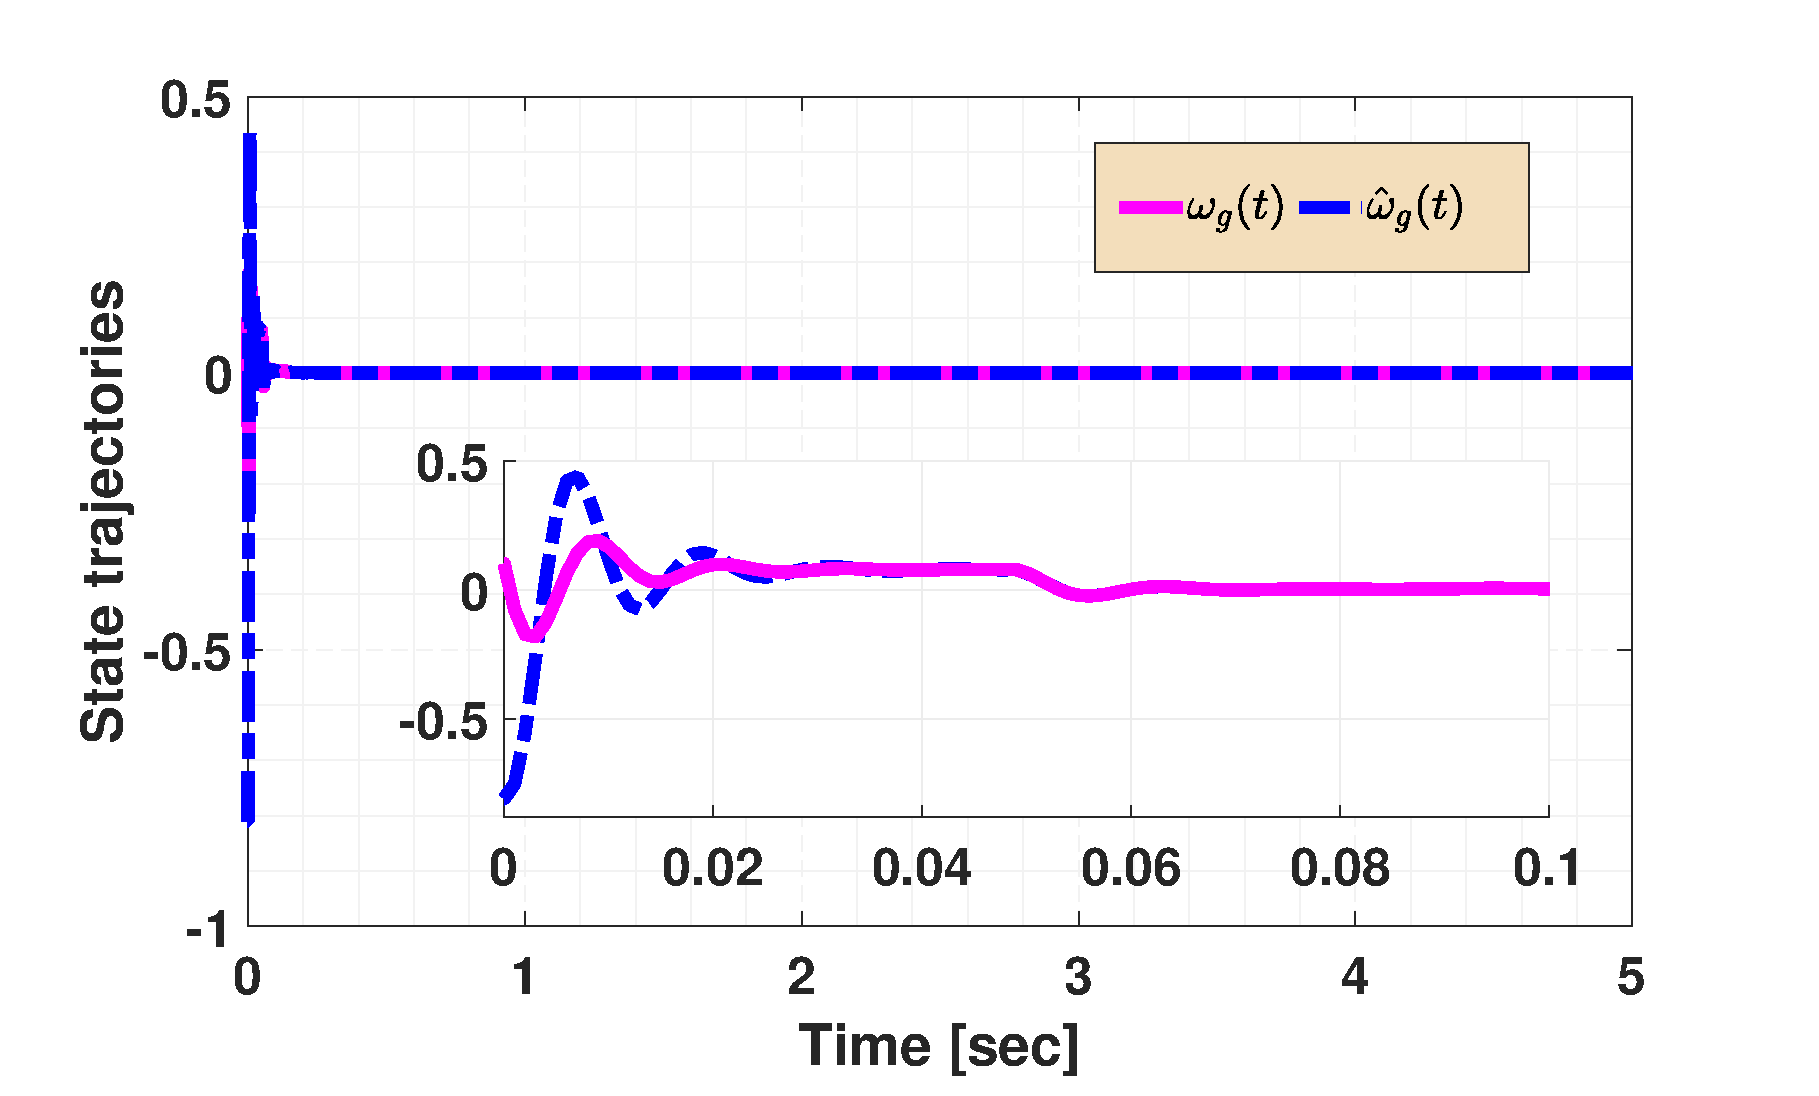
\includegraphics[width=8.6cm,height=6cm]{x1.eps}}
    \caption{ }
    \end{subfigure}
    \begin{subfigure}[b]{0.5\textwidth}
    \centerline{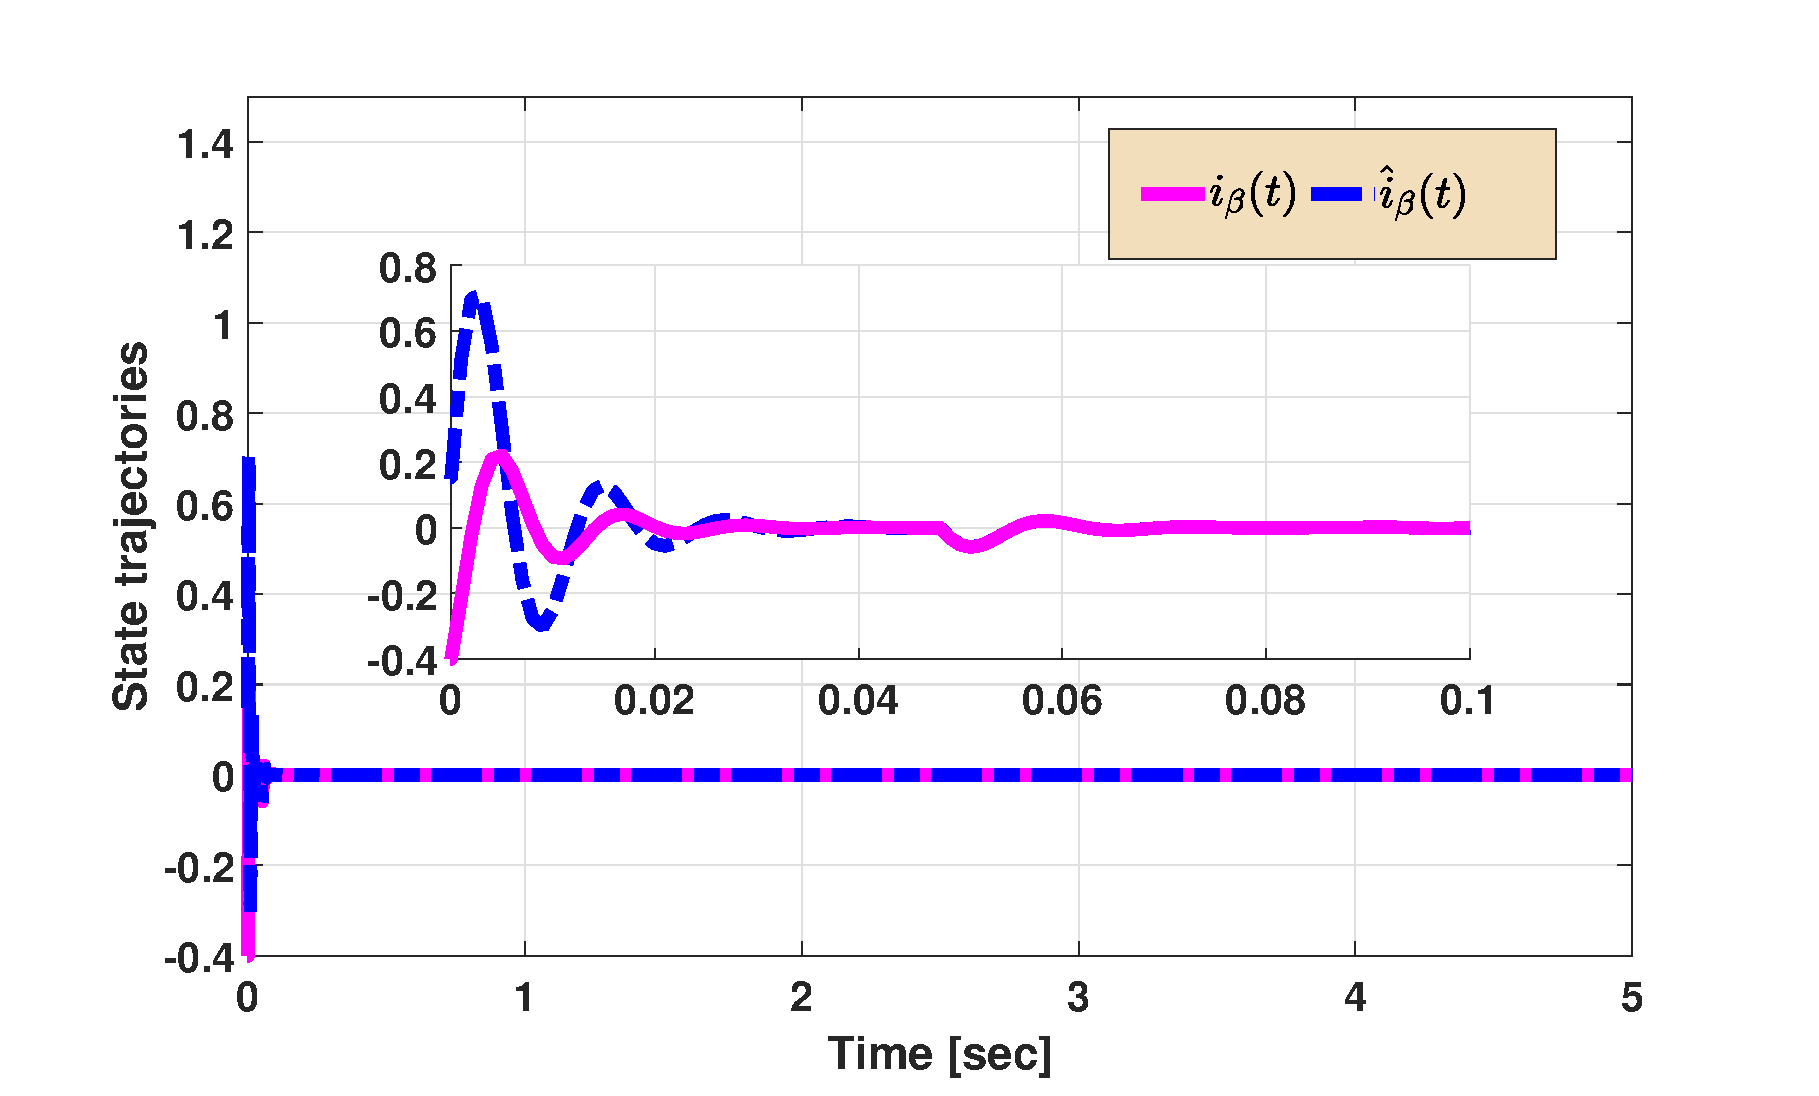
\includegraphics[width=8.6cm,height=6cm]{x2.eps}}
    \caption{ }
    \end{subfigure}
    \caption{(a) Dynamic behavior of $\omega_g(t)$ and its observer $\hat{\omega}_g(t)$ for Case I  (b) Dynamic behavior of $i_\beta(t)$ and its observer $\hat{i}_\beta(t)$ for Case I.} \label{F1}
    \end{figure}
    \begin{figure}[!ht]
    \begin{subfigure}[b]{0.5\textwidth}
    \centerline{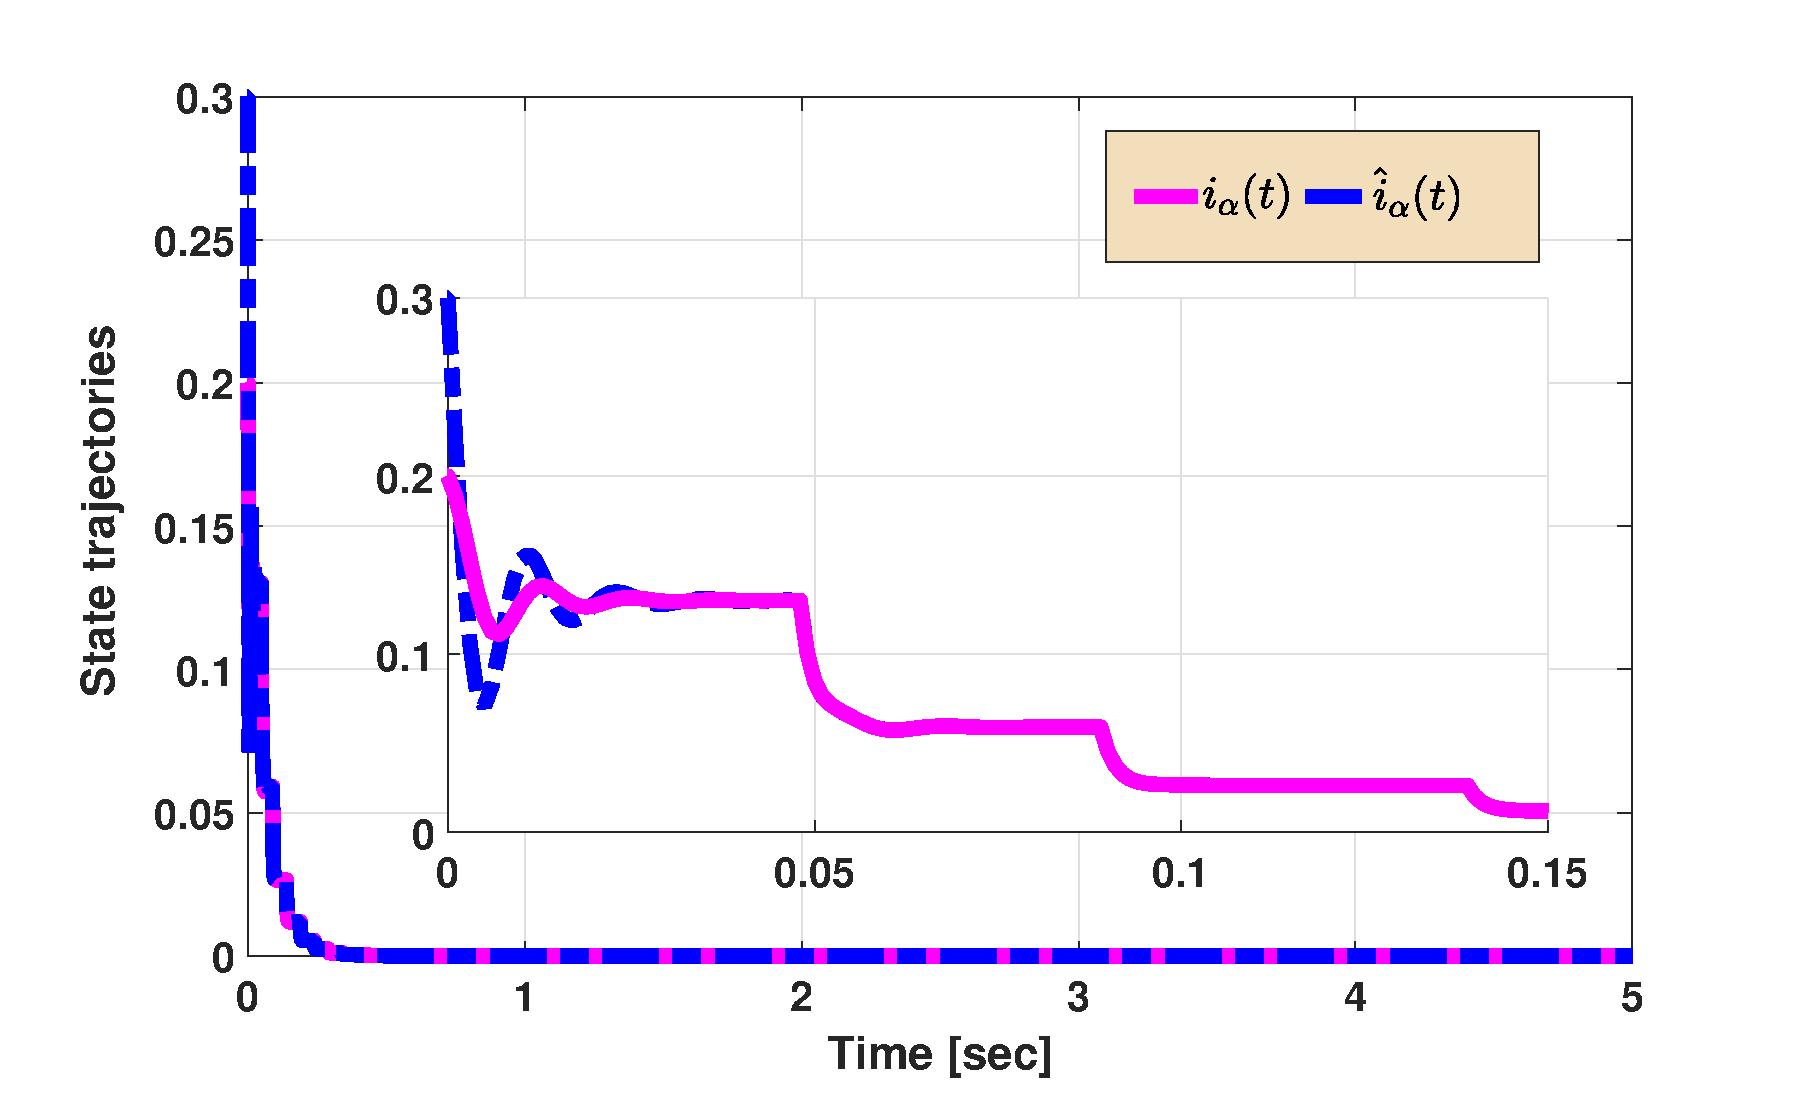
\includegraphics[width=8.6cm,height=5.8cm]{x3.eps}}
    \caption{ }
    \end{subfigure}
    \begin{subfigure}[b]{0.5\textwidth}
    \centerline{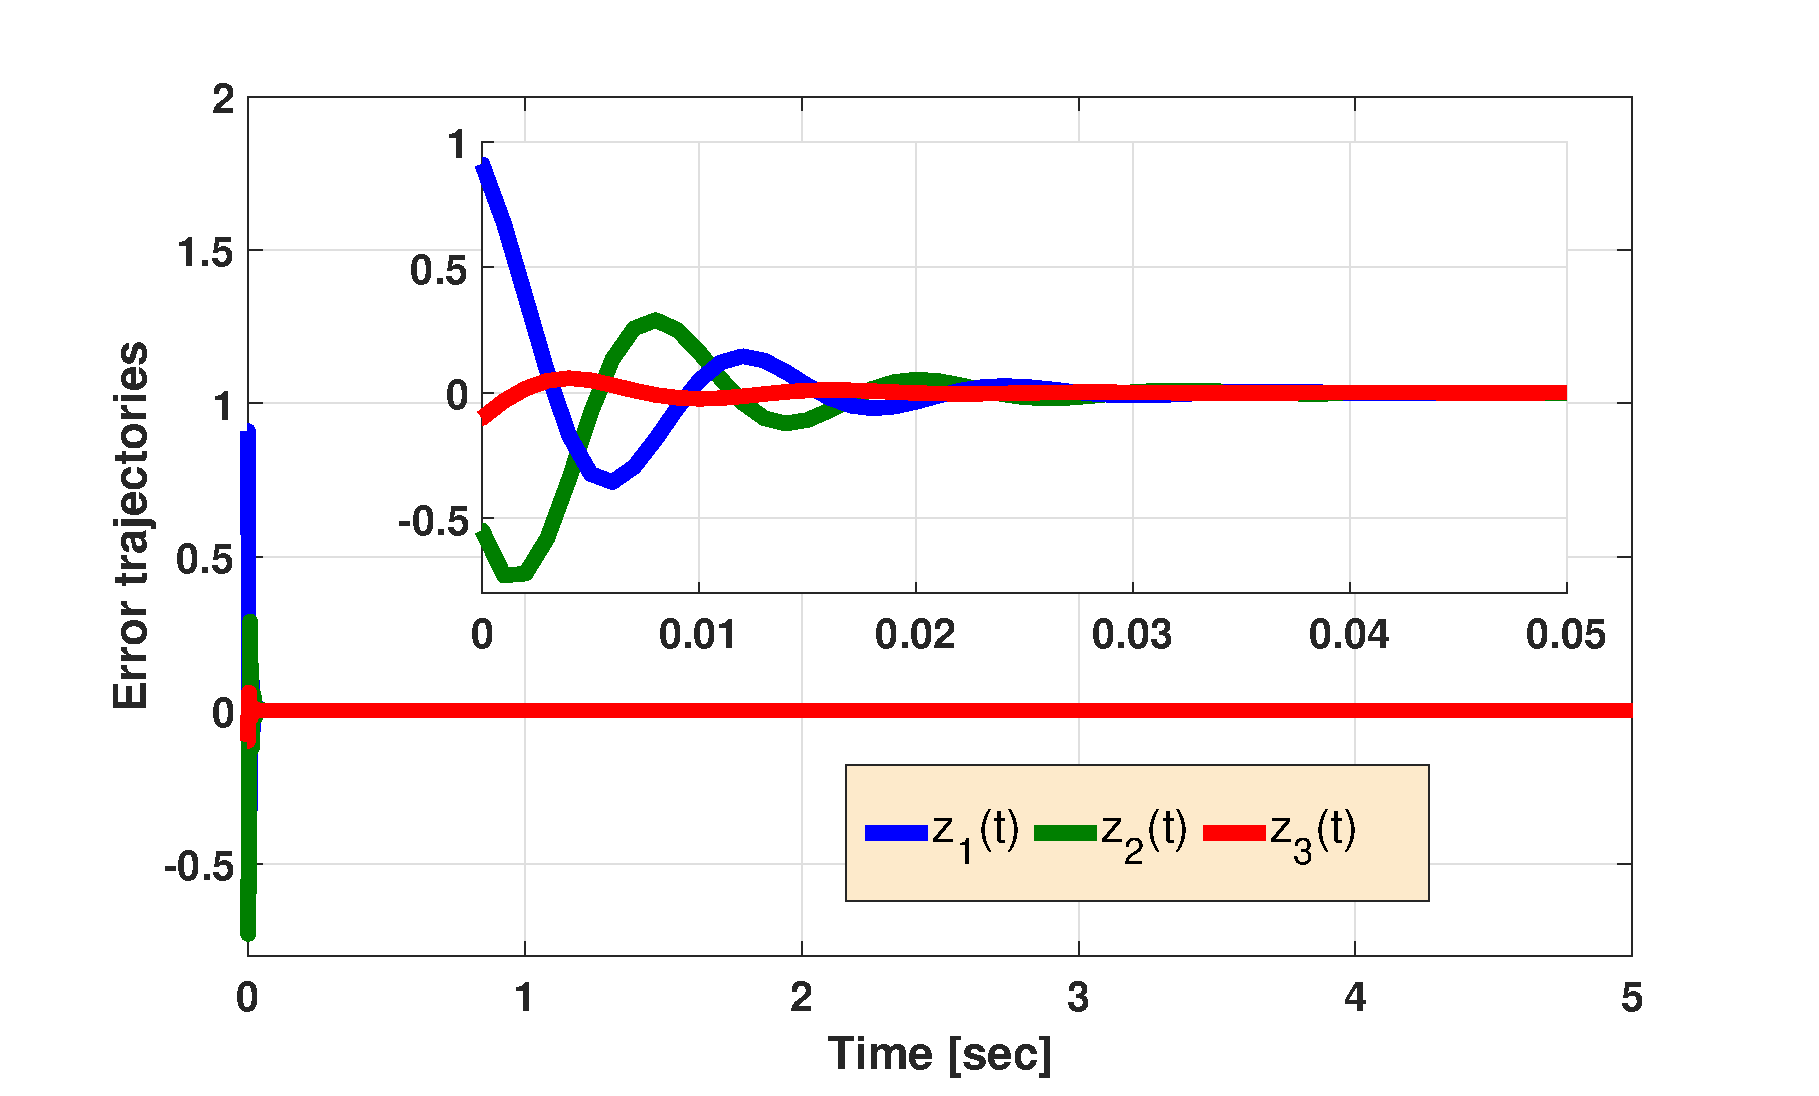
\includegraphics[width=8.6cm,height=5.8cm]{z1.eps}}
    \caption{ }
    \end{subfigure}
    \caption{(a) Dynamic behavior of $i_\alpha(t)$ and its observer $\hat{i}_\alpha(t)$ for Case I  (b) Error trajectories between the state $x(t)$ and their observer state $\hat{x}(t)$ for Case I.} \label{F2}
\centering
  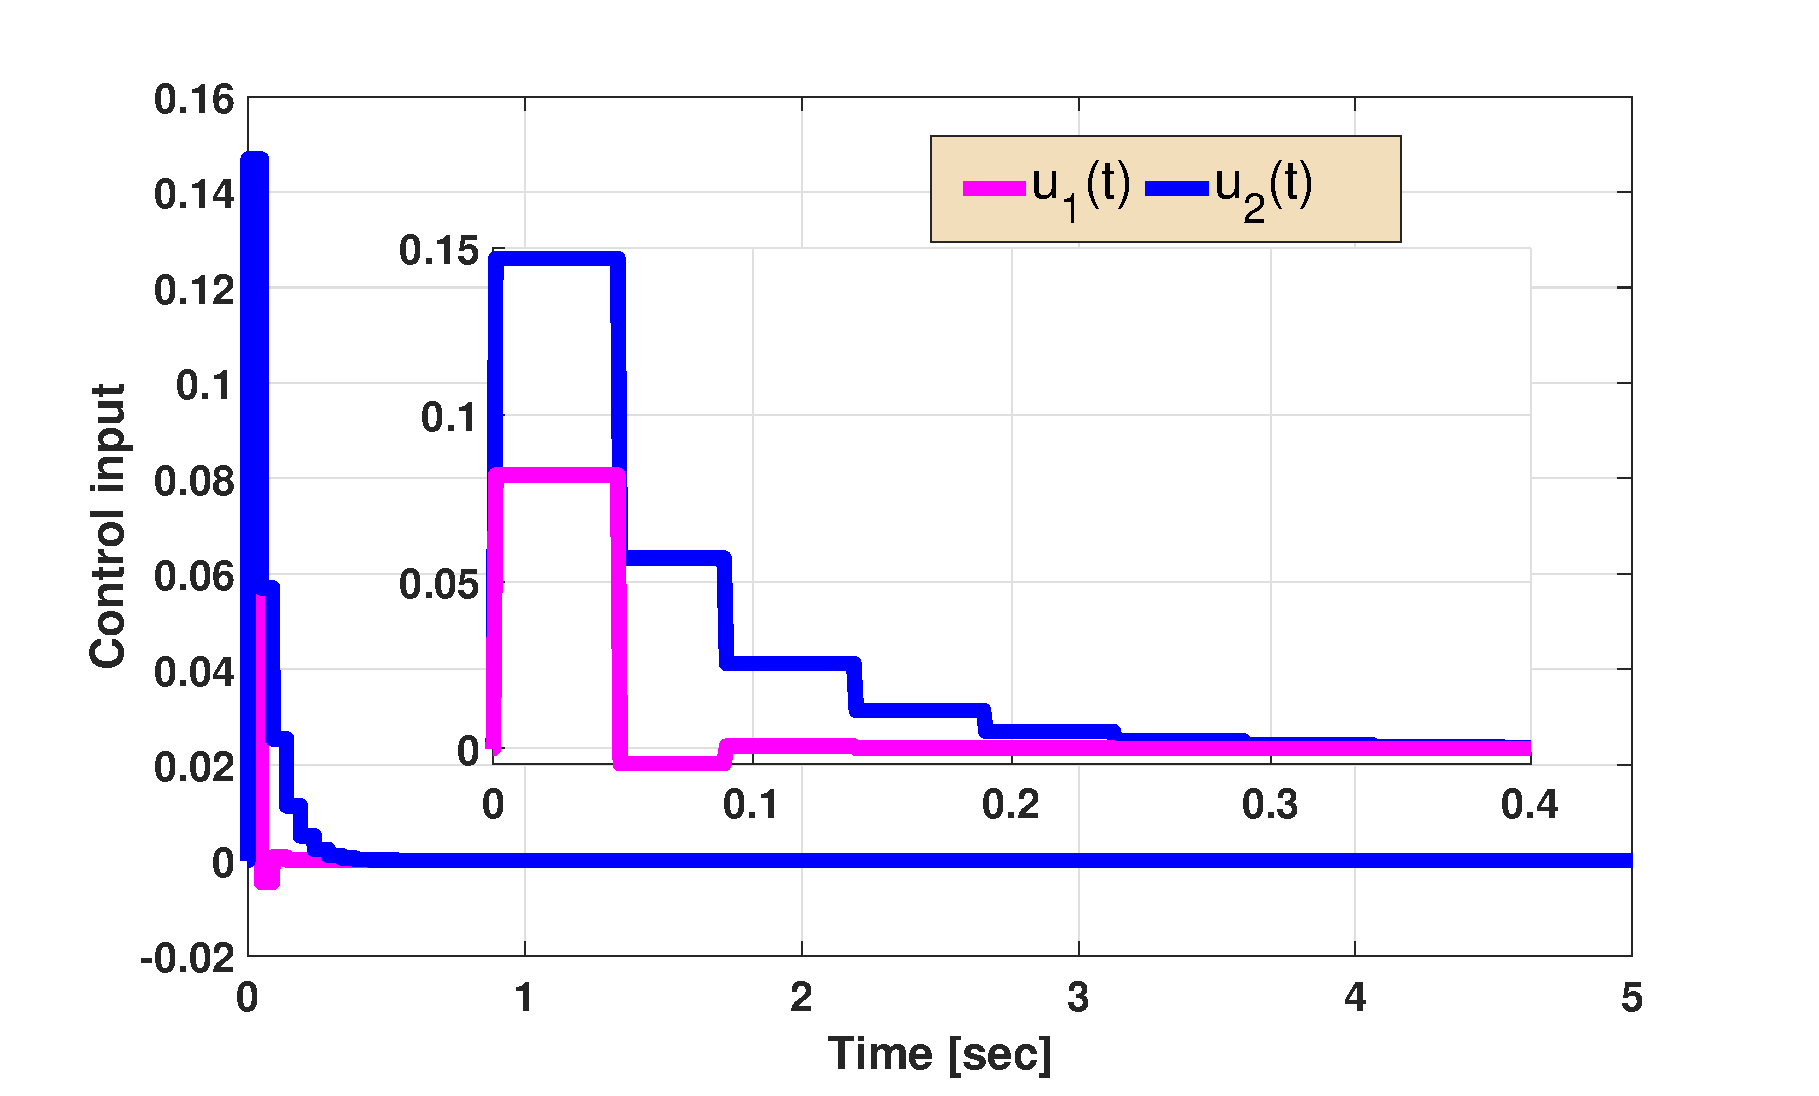
\includegraphics[height=5.8 cm,width=11.5cm]{u.eps}
\caption{Control input signals for Case I.}
\label{F5}
\vspace{-0.2cm}
\end{figure}
Next, utilizing the $\mathcal{SVD}$ technique, the matrix $\mathrm{C}_1=\mathrm{C}_2=\mathrm{C}$ is expressed as $\mathrm{C}=\mathbb{O}\big[ \mathbb{S}\;\;0 \big]\mathbb{V}^T$ with $\mathbb{V}=
\begin{bmatrix}
  1&   0 &   0\\
  0&   1&    0\\
  0&   0&    1
\end{bmatrix}$, $\mathbb{S}=\big[ 1\;\;0\;\;0 \big]$, and $\mathbb{O}=1$.
Further, we provide the following algorithm to calculate the maximum upper bound of the sample period $\tau_{M}$. This algorithm utilizes the MATLAB YALMIP toolbox to solve the LMIs \eqref{44}-\eqref{49} in Theorem \ref{Thm2}.\\
{\bf Algorithm 1:}\\
{\bf Step 1} For pre-given constants $\tau_m>0$, and select the appropriate parameters $\epsilon_1,\epsilon_2>0$, and $\hbar_1,\hbar_2>0$.\\
{\bf Step 2} Choose a suitably small step size value $h$ and set the initial value $\tau_{M0}=\tau_m+h$ for $\tau_{M}$.\\
{\bf Step 3} Let $n$ be integer counter with initial value $n=0$, and $\widehat{\tau}=nh+\tau_{M0}$.\\
{\bf Step 4} Use YALMIP Toolbox on MATLAB to solve the provided LMIs \eqref{44}-\eqref{49} with specified $\widehat{\tau}=\tau_{M}$. \\
{\bf Step 5} If a feasible solution exists, set $n=n+1$, then,  return to Step 2. Otherwise, proceed to Step 6.\\
{\bf Step 6} Output $\tau_{M}=\widehat{\tau}-h$, which is maximum upper bound of the sampling period.
\begin{figure}[h]
    \begin{subfigure}[b]{0.5\textwidth}
    \centerline{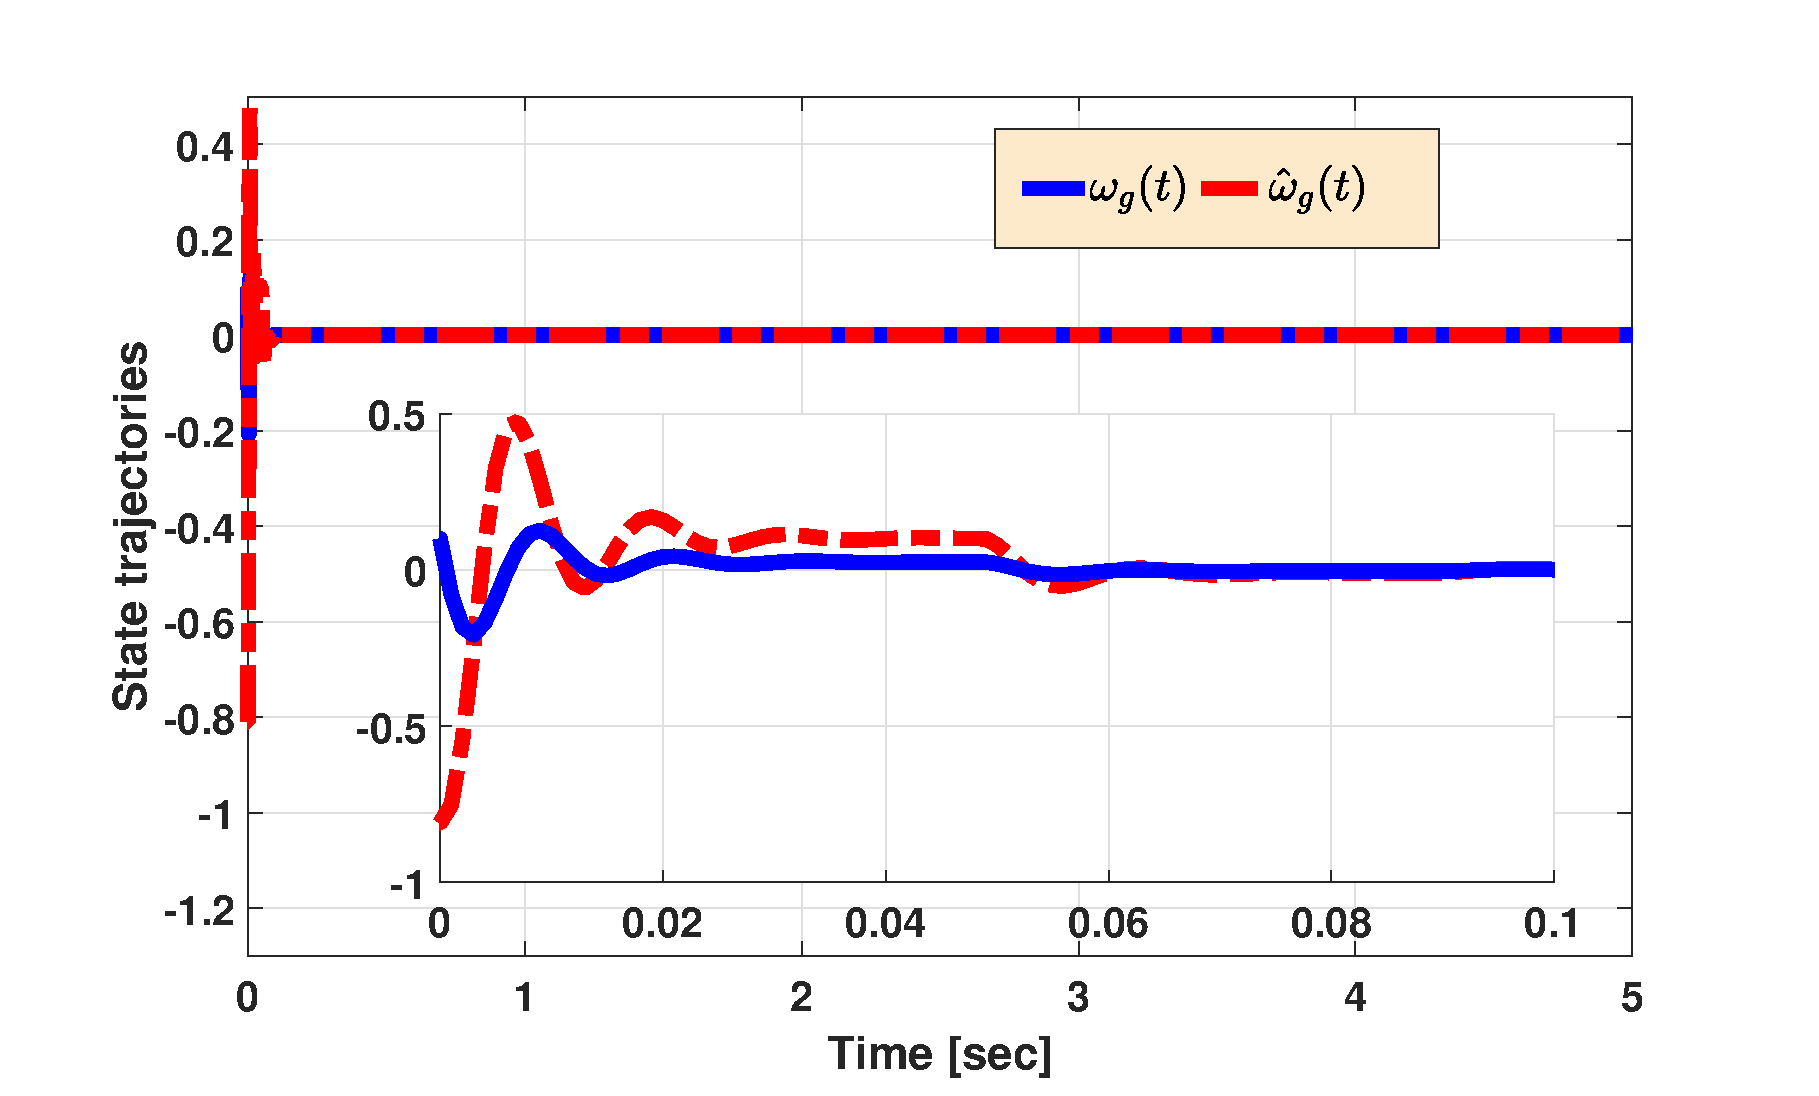
\includegraphics[width=8.6cm,height=5.8cm]{xx1.eps}}
    \caption{ }
    \end{subfigure}
    \begin{subfigure}[b]{0.5\textwidth}
    \centerline{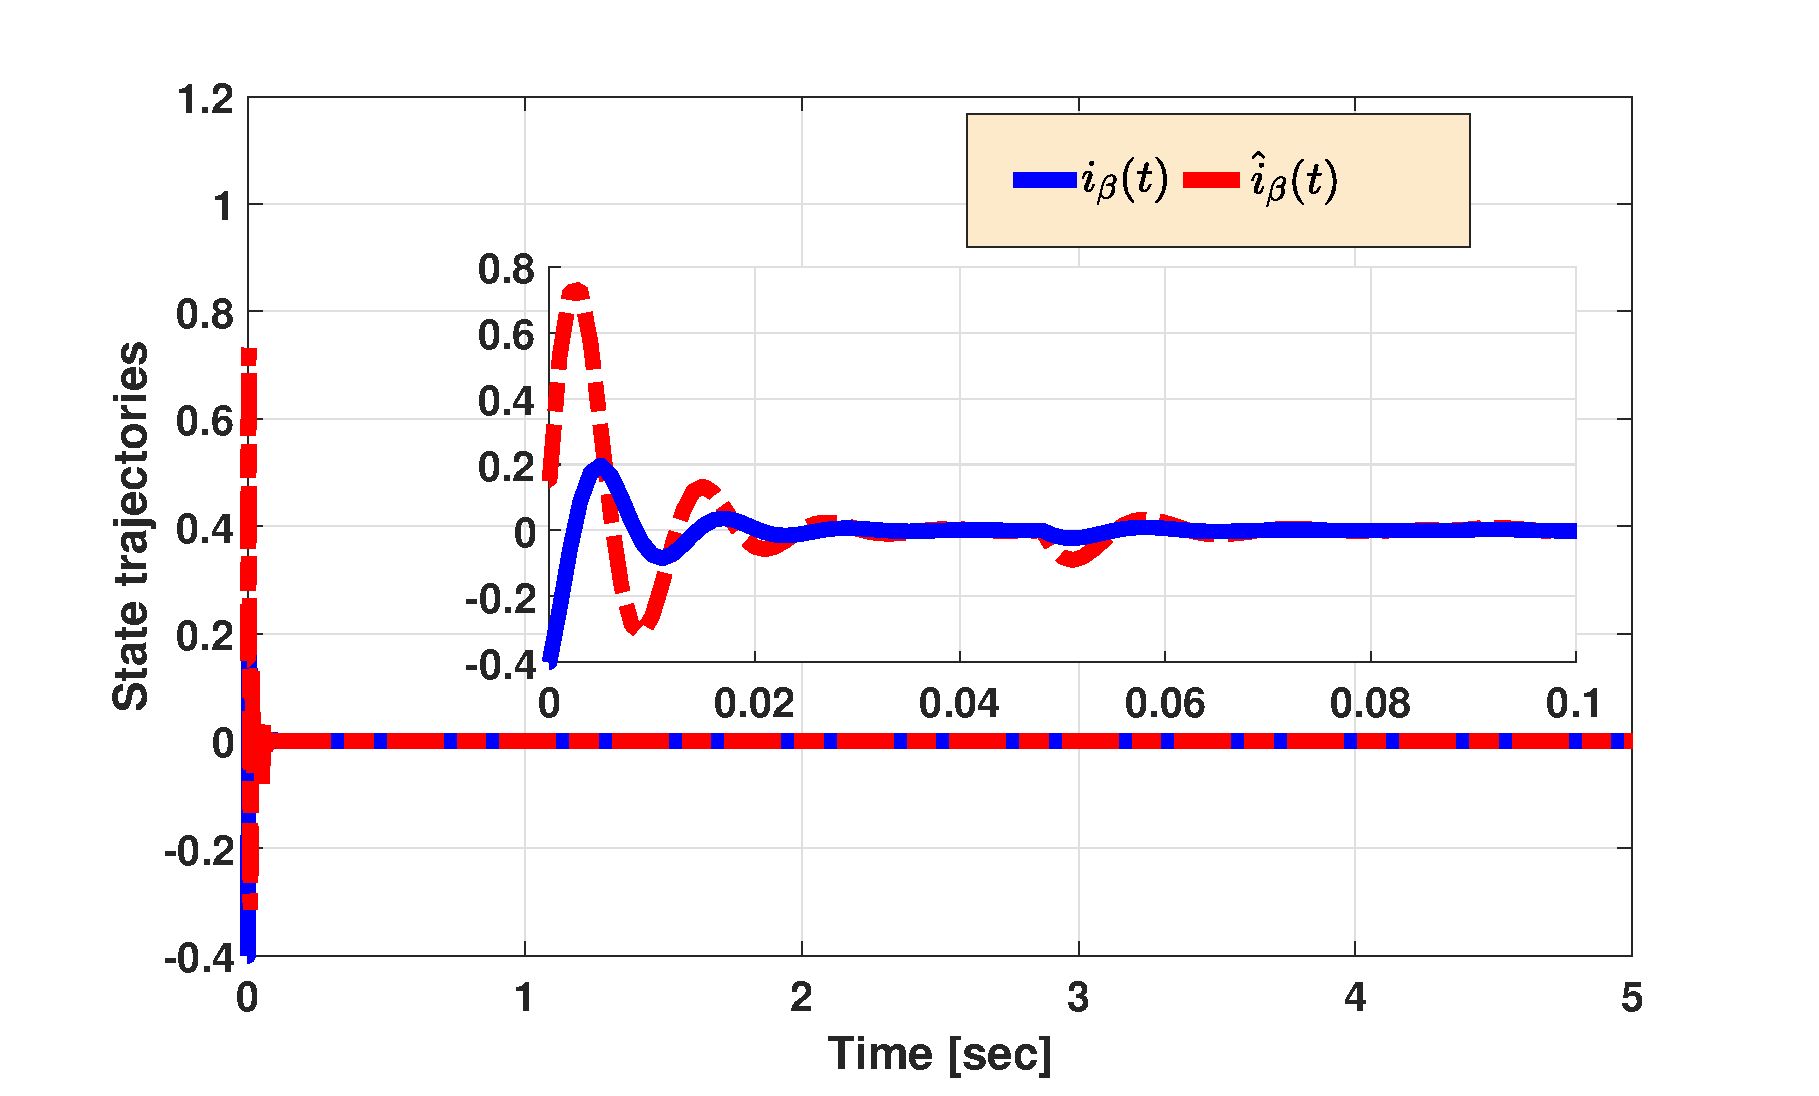
\includegraphics[width=8.6cm,height=5.8cm]{xx2.eps}}
    \caption{ }
    \end{subfigure}
    \caption{(a) Dynamic behavior of $\omega_g(t)$ and its observer $\hat{\omega}_g(t)$ for Case II  (b) Dynamic behavior of $i_\beta(t)$ and its observer $\hat{i}_\beta(t)$ for Case II.} \label{F3}
    \vspace{-0.3cm}
    \end{figure}
    \begin{figure}[h]
    \begin{subfigure}[b]{0.5\textwidth}
    \centerline{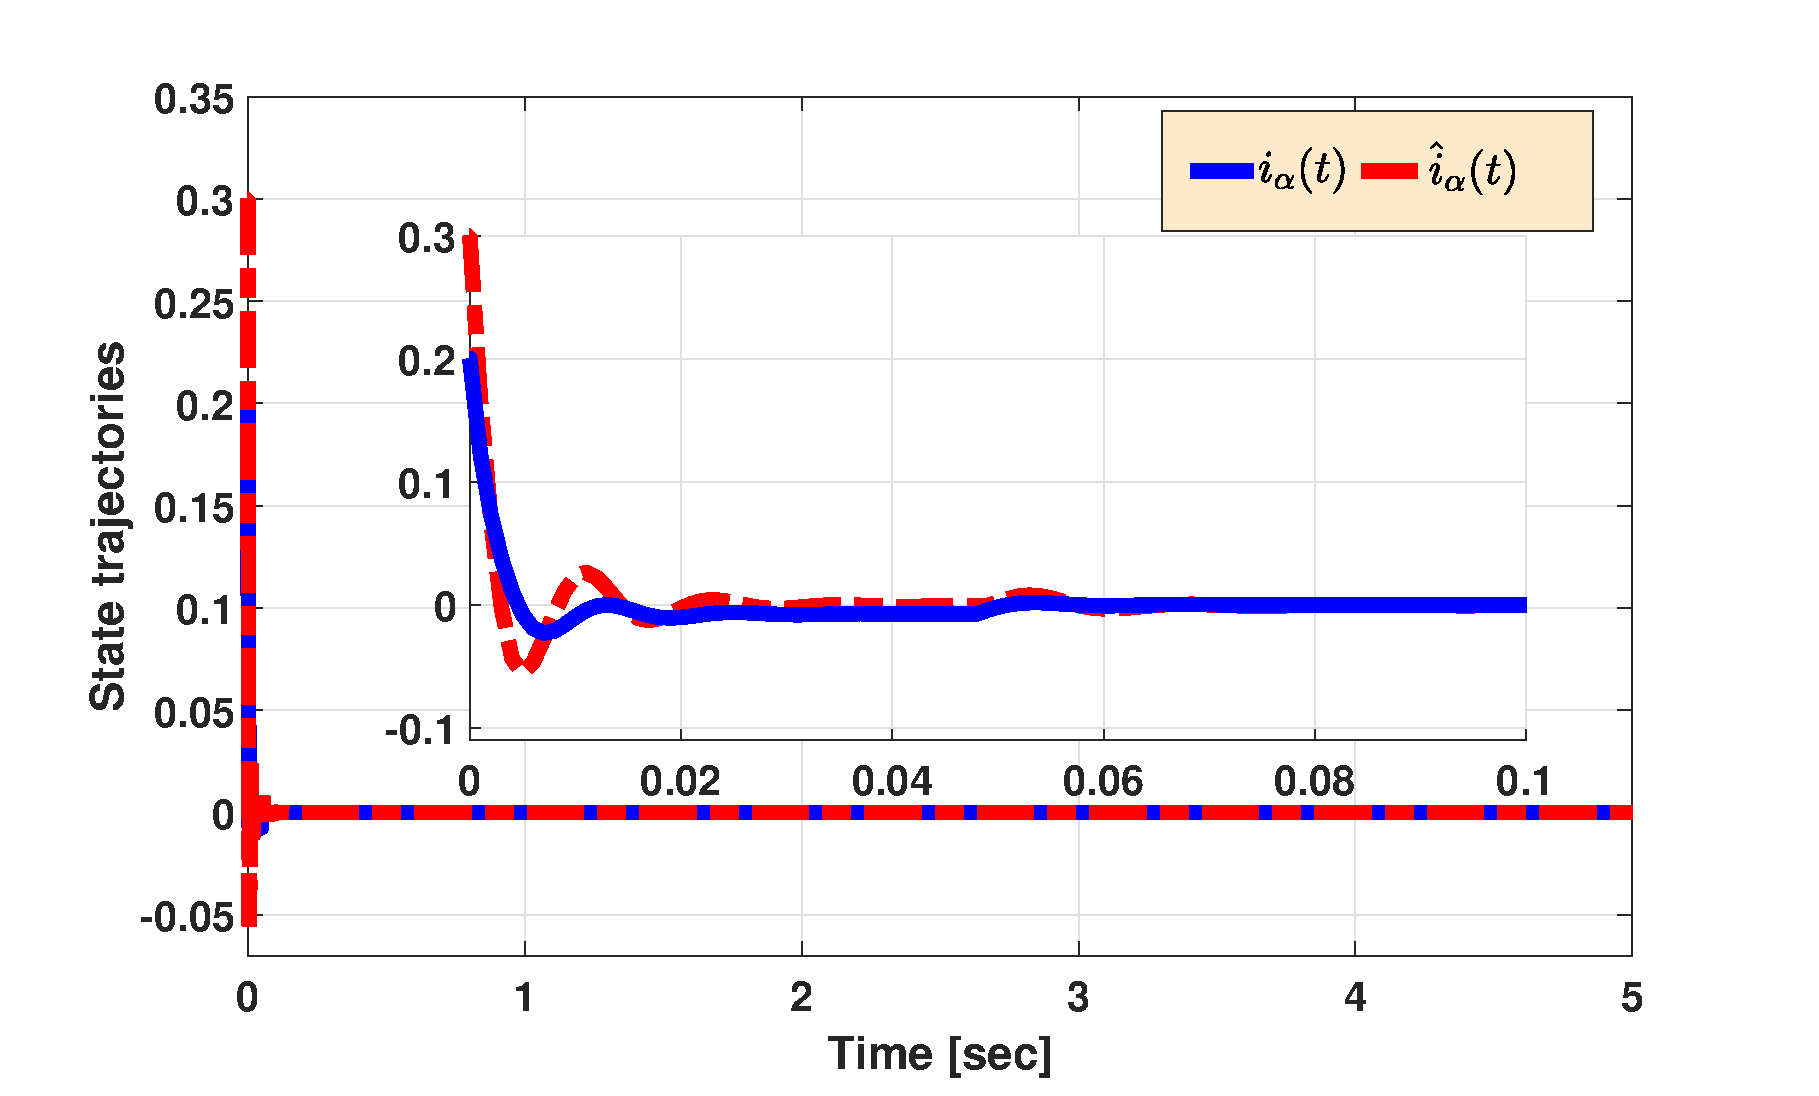
\includegraphics[width=8.6cm,height=5.8cm]{xx3.eps}}
    \caption{ }
    \end{subfigure}
    \begin{subfigure}[b]{0.5\textwidth}
    \centerline{\includegraphics[width=8.6cm,height=5.8cm]{zz1.eps}}
    \caption{ }
    \end{subfigure}
    \caption{(a) Dynamic behavior of $i_\alpha(t)$ and its observer $\hat{i}_\alpha(t)$ for Case II  (b) Error trajectories between the state $x(t)$ and their observer state $\hat{x}(t)$ for Case II.} \label{F4}
    \end{figure}
    \begin{figure}[h]
\centering
  \includegraphics[height=5.5 cm,width=11.5cm]{uu.eps}
\caption{Control input signals for Case II.}
\label{F10}\vspace{-0.5cm}
\end{figure}

Following Algorithm 1 and the solution of the LMIs described in Theorem \ref{Thm2}, we have determined the maximum upper bound of the sample period (MUBSP) as well as the corresponding controller and observer gain matrices that are given in Table \ref{Table-6}.
\begin{table*}[!ht]
\centering
\caption{Numerical solution for Theorem \ref{Thm2} with $\tau_m=10^{-5}s$ }
\label{Table-6}
\begin{tabular}{l|c|c|c|c}   \hline
Case & $\begin{bmatrix}\mathrm{K}_1\\\mathrm{K}_2\end{bmatrix}$&$\begin{bmatrix}\mathrm{H}_1\\\mathrm{H}_2\end{bmatrix}$&$\tau_M$&NODVs\\\hline
I  &
$\begin{bmatrix}
 -0.0672 &  -0.0341 &  -0.0005\\
   -0.0005 &  -0.0003&    0.0044
\end{bmatrix}$
& $\begin{bmatrix}
 -0.0007\\
    0.0344\\
   -0.0001
\end{bmatrix}
\vspace{0.01cm}
$&0.454&$734.5n^2+38.5n+2nm$\\
&
$\begin{bmatrix}
   -0.0671  & -0.0341  & -0.0005\\
   -0.0005  & -0.0004  &  0.0045
\end{bmatrix}
$& $\begin{bmatrix}
   -0.0007\\
    0.0346\\
    0.0004
\end{bmatrix}
$\vspace{0.01cm}&&\\
\hline
II  & $\begin{bmatrix}
-0.0460 &  -0.0384  &  0.0058\\
    0.0004&   -0.0036&   -0.0251
\end{bmatrix}$
&$\begin{bmatrix}
0.1902\\
   39.0625\\
    2.9989
\end{bmatrix}$
\vspace{0.01cm}&&\\
 &
$\begin{bmatrix}
-0.0460 &  -0.0384 &   0.0058\\
    0.0004 &  -0.0036 &  -0.0251
\end{bmatrix}$
&$\begin{bmatrix}
0.0719\\
   39.7090\\
   -5.8775
\end{bmatrix}$
&0.461&$812.5n^2+38.5n+2nm$\\
\hline
\end{tabular}
\vspace{-0.4cm}
\end{table*}

{From Table \ref{Table-6}, the number of decision variables (NODVs) in Case I for Theorem \ref{Thm2} is $734.5n^2+38.5n+2nm$, which is smaller than $812.5n^2+38.5n+2nm$ in Case II for Theorem \ref{Thm2}. That indicates case I is more relaxed with relatively small NODVs. Meantime, the MUBSP is further enhanced by case II at the expense of increased computational intricacy. Therefore, acquiring the MUBSP at a minimal computational burden is the direction of future research.}



According to the observer gain matrices as given in Table \ref{Table-6} and initial condition $x(0)=[ 0.1\;\;-0.4\;\;0.2 ]^T$ and $\hat{x}(0)=[-0.81\;\;0.15\;\;0.3 ]^T$, the simulation results of considered closed-loop {Takagi-Sugeno} fuzzy PMSG-based WTS \eqref{7} and its state observer \eqref{9} are shown in Figs.\ref{F1}-\ref{F10}. Based on these figures, the controller designed in \eqref{11} ensures the smooth convergence of the fuzzy augmented closed-loop system given by \eqref{14}. The dynamic responses of the mechanical rotational speed $\omega_g(t)$ and their estimations $\hat{\omega}_g(t)$ are shown in Fig.\ref{F1}(a) and Fig.\ref{F3}(a), respectively. Fig.\ref{F1}(b) and Fig.\ref{F3}(b) demonstrate the stator current $\hat{i}_\beta(t)$ and their estimations $\hat{i}_\beta(t)$, and  Fig.\ref{F2}(a) and Fig.\ref{F4}(a) provide the stator current $\hat{i}_\alpha(t)$ and their estimations $\hat{i}_\alpha(t)$, respectively. Meanwhile, the dynamics of the error states $z(t)$ and control inputs $u(t)$ are revealed in Fig.\ref{F2}(b), Fig.\ref{F4}(b) and Fig.\ref{F5} and Fig.\ref{F10}, respectively. From those figures, we confirm that the designed FSDO can effectively estimate the presented wind turbine model. Hence, it is evident that the designed controller in \eqref{11} ensures the asymptotic stability of the closed-loop system \eqref{14}.

{Next, to demonstrate the effectiveness of the proposed controller, we compare our findings with those of previous research as documented in \cite{sub1}. In \cite{sub1}, the observer state can take almost $0.06s \sim0.08s$ to estimate the system state (see Figs. ${2}$-${4}$ in \cite{sub1}) exhibiting higher overshoot within the $0.4s \sim3.5s$ range. But, our designed observer estimates the system state within 0.045s (see Figs. \ref{F1}-\ref{F10}) and less overshoot within the range $0.8s$, which is better performance than the existing research \cite{sub1}. In conclusion, our study has shown that the proposed fuzzy observer offers superior performance in terms of faster convergence rates, smoother control signals, and reduced overshoot when compared to the prior research \cite{sub1}.} As a result, we have successfully achieved our primary research objectives.
\subsection{Numerical Comparisons}
In this subsection, we demonstrate the validity and superiority of the proposed new integral inequality for analyzing the stability of sampled-data linear system \eqref{51} with the following parameters.\\
Comparison \;1:
$\mathrm{A}=
\begin{bmatrix}
 -2&  0 \\
  0&   -0.9
\end{bmatrix}$,
$\mathrm{A}_s=
\begin{bmatrix}
 -1&   0 \\
  -1&   -1
\end{bmatrix}$\\\\
Comparison \;2:
$\mathrm{A}=
\begin{bmatrix}
 0&  1 \\
  1&  0
\end{bmatrix}$,
$\mathrm{A}_s=
\begin{bmatrix}
 0&   0 \\
  -2&  -2
\end{bmatrix}$\\\\
Comparison \;3:
$\mathrm{A}=
\begin{bmatrix}
 -1&  -1 \\
  -1&  -2
\end{bmatrix}$,
$\mathrm{A}_s=
\begin{bmatrix}
 0&   0 \\
  -1&  -2
\end{bmatrix}$.\\
In the following, we revealed the superiority of the presented approach in this study. By solving the LMIs in Corollary \ref{cor1} using the parameter values in comparison examples 1-3, the MUBSP $\tau_M$ can be obtained under different $\tau_m$, and the relevant research results are tabulated in Table \ref{Table-7}-\ref{Table-9}.
\vspace{-0.3cm}
\begin{table}[!ht]
\centering
\caption{The obtained MUBSP $\tau_M$ with $\tau_m=10^{-5}$}
\label{Table-7}
\begin{tabular}{l|ccccccc} \hline\label{T5}
Method&\cite{example1a}&\cite{example1b}&\cite{example1c}&{\cite{Steve-1}}&Corollary \ref{cor1}\\\hline
Comparison \;1  &$2.8539$&$2.9239$& $2.9776$& {$2.9918$}& $\mathbf{3.008}$\\
\hline
\end{tabular}
\centering
\caption{The obtained MUBSP $\tau_M$ with $\tau_m=10^{-5}$}
\label{Table-8}
\begin{tabular}{l|ccccc} \hline\label{T5}
Method&\cite{example2a}&\cite{example2b}&\cite{example2c}&Corollary \ref{cor1}\\\hline
Comparison \;2 &$0.0484$&$1.0956$& $1.0971$& $\mathbf{1.098}1$\\
\hline
\end{tabular}
\centering
\caption{The obtained MUBSP $\tau_M$ with $\tau_m=10^{-2}$}
\label{Table-9}
\begin{tabular}{l|ccccc} \hline\label{T5}
Method&\cite{example2b}&\cite{example3b}&\cite{example3c}&Corollary \ref{cor1}\\\hline
Comparison \;3  &$2.1881$&$3.2156$& $4.0868$& $\mathbf{4.1611}$\\
\hline
\end{tabular}
\end{table}

The results from the tables above, as shown in Corollary \ref{cor1}, demonstrate larger ranges of sampling periods compared to those reported in existing literature. It can be observed instinctively from Table \ref{Table-7}-\ref{Table-9} that the obtained result is less conservatism than that of studies \cite{example1a,example1b,example1c, Steve-1, example2a, example2b,example2c,example3b,example3c}. To sum up, the comparative numerical analyses have effectively showcased the advantages of the proposed method in this study.
\vspace{-0.5cm}
\section{Conclusion}\vspace{-0.3cm}
In this study, the FSDO has been designed to estimate the unmeasurable states in PMSG-based WTS, where the premise variable of the systems, observer, and controller are asynchronous. First, a novel AFBII technique (see Lemma \ref{Lemma3}) has been proposed to estimate the integral terms. Then, a DSLLKF \eqref{22} has been developed to utilize the complete details of the actual sampling pattern. Next, based on the $\mathcal{SVD}$ procedure and AFBII technique, some sufficient conditions have been acquired to guarantee the asymptotic stability for the considered augmented closed-loop system. It is worth mentioning that the mismatched premise conditions have been well considered while deriving the main results of this study, which can enormously reduce the conservatism of the outcomes. At last, the validity and feasibility of the considered wind turbine model have been verified through the design example, which reveals good transient performance and outperforms than prior result \cite{sub1}. What is more, some comparative examples have been provided to prove the superiority of the proposed method, which demonstrates that the proposed AFBII technique can successfully minimize the conservativeness of the obtained results.

{In this study, we have assumed $\mathrm{L}_{\alpha}=\mathrm{L}_{\beta}$(smooth air-gap case) in the modeling of PMSG-based WTS. Accordingly, in our future work,  we will soon focus on the study of nonfragile FSDO design for {Takagi-Sugeno} fuzzy uncertain PMSG-based WTS with nonsmooth air-gap junctions case $(\mathrm{L}_{\alpha}\neq\mathrm{L}_{\beta})$. In addition to that, it is noted that the control input matrix $\mathrm{B}=\mathrm{B}_{1}=\mathrm{B}_{2}$ of the proposed {Takagi-Sugeno} fuzzy systems \eqref{7} is the same for each fuzzy rule, which broadly exists in numerous practical systems, such as mass-spring system \cite{Mass}, truck-trailer system \cite{example1a}, ship propulsion system \cite{lem1}, and so on. Of course, we have observed few works that have presented results of {Takagi-Sugeno} fuzzy systems with different control input matrices \cite{FD-1}. Inspired by \cite{FD-1}, we will study the non-synchronous piecewise affine FSDO for other nonlinear systems through {Takagi-Sugeno} fuzzy affine models, specifically when the restriction of control input matrices being the same is relaxed in future research. Another possible future work will mainly focus on extending the proposed method to other nonlinear systems, such as  autonomous marine systems \cite{UMV-1}, autonomous vehicle systems \cite{UMV-2}, tunnel diode circuit systems \cite{UMV-3}, and so on.}


\vspace{-0.5cm}
\section*{Acknowledgement}\vspace{-0.2cm}
This work was supported in part by the Basic Science Research Program under Grant NRF-2016R1A6A1A03013567 and Grant NRF-2021R1A2B5B01001484 and by the framework of International Cooperation Program under Grant NRF-2022K2A9A2A06045121 through the National Research Foundation of Korea (NRF) funded by the Ministry of Education.
\vspace{-0.5cm}
\begin{thebibliography}{00}\frenchspacing
\balance
\bibitem{wind1}
R.E. Precup, T. Kamal, and S.Z. Hassan, ``{\em Advanced control and optimization paradigms for wind energy systems,}'' Springer, 2019.

\bibitem{wind3}
A. T. Azar and N.A. Kamal, ``{\em Renewable energy systems: Modelling, optimization and control,}'' Elsevier, 2021.

\bibitem{wind2}
S. Kuppusamy, Y.H. Joo, and H.S. Kim, ``Fault-tolerant load frequency control for DFIG-based interconnected wind power systems'',  {\em Information Sciences,} vol.~582, pp. 73-88, 2022.

\bibitem{wind4}
M. Chinchilla, S. Arnaltes, and J.C. Burgos, ``Control of permanentmagnet generators applied to variable-speed wind-energy systems connected to the grid,'' {\em IEEE Transactions on Energy Conversion,} vol.~21, no.~1, pp.~130–135, 2006.

\bibitem{wind5}
R. Errouissi and A. Al-Durra, ``A novel PI-type sliding surface for PMSG-based wind turbine with improved transient performance'', {\em IEEE Transactions on Energy Conversion,} vol. 33, no. 2, pp. 834-844, 2017.

\bibitem{wind6}
H. Ye, B. Yue, X. Li, K. Strunz, ``Modeling and simulation of multi-scale transients for PMSG-based wind power systems,'' {\em Wind Energy}, vol. 20 no. 8, pp. 1349–1364, 2017.

\bibitem{wind7}
H. Matayoshi, A.M. Howlader, M. Datta, and T. Senjyu, ``Control strategy of PMSG based wind energy conversion system under strong wind conditions,''  {\em Energy for Sustainable Development,} vol. 45, pp. 211–218, 2018.

\bibitem{wind8}
E. Kamal, A. Aitouche, R. Ghorbani, and M. Bayart, ``Robust fuzzy fault-tolerant control of wind energy conversion systems subject to sensor faults,'' {\em IEEE Transactions on Sustainable Energy,} vol. 3, no. 2, pp. 231– 241, 2012.

\bibitem{EDI-1}
{M.L. Tomescu,  S. Preitl, R.E. Precup, and J.K. Tar, ``Stability analysis method for fuzzy control systems dedicated controlling nonlinear processes,'' {\em Acta Polytechnica Hungarica,} vol. 4, no. 3, pp. 127-141, 2007.}

\bibitem{EDI-2}
{R.E. Precup, S. Preitl, E. Petriu, C.A. Bojan-Dragos, A.I. Szedlak-Stinean, R.C. Roman, and E.L. Hedrea, ``Model-based fuzzy control results for networked control systems,'' {\em  Reports in Mechanical Engineering,} vol. 1, no. 1, pp. 10-25, 2020.}

\bibitem{EDI-3}
{Y. Feng, M. Wu, L. Chen, X. Chen, W. Cao, S. Du, and W. Pedrycz, ``Hybrid intelligent control based on condition identification for combustion process in heating furnace of compact strip production,'' {\em  IEEE Transactions on Industrial Electronics,} vol. 69, no. 3, pp. 2790-2800, 2022.}

\bibitem{fuzzy1}
T. Takagi and M. Sugeno, ``Fuzzy identification of systems and its applications to modeling and control,'' {\em IEEE Transactions on Systems, Man, and Cybernetics,} no. 1, pp. 116–132, 1985.

\bibitem{R3-1}
{X. Xu, Y. Shen, W. Pedrycz, Y. Li, and G. Wu, ``Granular fuzzy rule-based modeling with incomplete data representation,'' {\em IEEE Transactions on Cybernetics}, vol. 52, no. 7, pp. 6420-6433, 2022.}

\bibitem{R3-2}
{A. Ramathilagam  and P. Pitchipoo, ``Modeling and development of fuzzy logic-based intelligent decision support system,'' {\em Romainian Journal of Information Sciemce and Technology}, vol. 25, no. 1, pp. 58-79, 2022.}

\bibitem{R3-3}
{A.I. Szedlak-Stinean, R.E. Precup, E.M. Petriu, R.C. Roman, E.L. Hedrea  and C.A. Bojan-Dragos, ``Extended Kalman filter and Takagi-Sugeno fuzzy observer for a strip winding system,'' {\em Expert Systems With Applications}, vol. 208, 118215, 2022.}







\bibitem{fuzzy0}
R.~Subramaniyam and Y.H. Joo, ``Passivity-based fuzzy ISMC for wind energy conversion systems with PMSG,'' {\em  IEEE Transactions on Systems, Man, and Cybernetics: Systems}, vol.~51, no.~4, pp.~2212-2220, 2021.

\bibitem{fuzzy2}
P.~Mani and Y.H. Joo, ``Fuzzy event-triggered control for back to back converter involved PMSG-based wind turbine systems'', {\em  IEEE Transactions on Fuzzy Systems,} vol.~30, no.~5, pp.~1409-1420, 2022.

\bibitem{fuzzy3}
S. Yan, Z. Gu, J.H. Park, and X. Xie, ``Adaptive memory event-triggered static output control of T-S fuzzy wind turbine systems'', {\em IEEE
Transactions on Fuzzy Systems,} vol. 30, no 9, pp. 3894 - 3904, 2022.



\bibitem{PMSM}
L.~Shanmugam  and Y.H. Joo, ``Design of interval type-2 fzzy-based sampled-data controller for nonlinear systems using novel fuzzy lyapunov functional and its application to PMSM'', {\em  IEEE Transactions on Systems, Man, and Cybernetics: System}, vol.~51, no.~1,  pp.~542-551, 2021.

\bibitem{Mass}
Z.~You, H. Yan, H. Zhang, L. Zeng, and M. Wang, ``Further stability criteria for sampled-data-based interval type-2 fuzzy systems via a refined two-side looped-functional method'', {\em   IEEE Transactions on Fuzzy Systems}, vol.~31, no.~1,  pp.~265--277, 2023.

\bibitem{vijay}
A. Stephen, R. Karthikeyan, C. Sowmiya, R. Raja, Ravi. P. Agarwal, ``Sampled-data controller scheme for multi-agent systems and its Application to circuit network,'' {\em Neural Networks,} 170, pp. 506-520, 2024.

\bibitem{PMSG1}
P.~Mani, J.H.~Lee, K.W.~Kang, and Y.H.~Joo, ``Digital controller design via LMIs for direct-driven surface mounted PMSG-based wind energy conversion system'', {\em IEEE Transactions on Cybernetics}, vol.~50, no.~7, pp.~3056-3067, 2020.

\bibitem{PMSG2}
L.~Shanmugam and Y.H.~Joo, ``Stabilization of permanent magnet synchronous generator-based wind turbine system via fuzzy-based sampled-data control approach'', {\em Information Sciences}, vol.~559, pp.~270--285, 2021.

\bibitem{vel1}
V.~Gandhi and Y.~H. Joo, ``T-S fuzzy sampled-data control for non-linear systems with actuator faults and its application to wind energy system'', {\em IEEE Transactions on Fuzzy Systems}, vol.~30, no.~2, pp.~462-474, 2022.

\bibitem{PMSG3}
S.  Kuppusamy and Y.H. Joo, ``Stabilization criteria for T-S fuzzy systems with multiplicative sampled-data control gain uncertainties'', {\em IEEE Transactions on Fuzzy Systems,} vol.~30, no.~10, pp.~4082-4092, 2022.

\bibitem{New-1}
{S. Arthanari and Y.H. Joo, ``Memory sampled-data control for T–S fuzzy-based permanent magnet synchronous generator via an improved looped functional'', {\em IEEE Transactions on Systems, Man, and Cybernetics: Systems,} vol.~53, no.~7, pp.~4417--4428, 2023.}


\bibitem{New-3}
{P.  Anbalagan and Y.H. Joo,  ``Fuzzy membership-function-dependent design of aperiodic sample-data control scheme for nonlinear PMSG-based WECS with quantization measurements via refined looped Lyapunov functional'', {\em Information Sciences,} vol.~661, 120149, 2024.}

\bibitem{New-2}
{R. Dutta and Y.H. Joo, ``Fuzzy memory sampled-data controller design for PMSG-based WECS with stochastic packet dropouts'', {\em IEEE Transactions on Fuzzy Systems,} vol.~31, no.~12, pp.~4421--4434, 2023.}

\bibitem{New-4}
{P.  Anbalagan and Y.H. Joo,  ``Nonfragile sampled-data control for interval type-2 fuzzy modeling of permanent magnet synchronous generator-based wind turbine systems'', {\em IEEE Transactions on Systems, Man, and Cybernetics: Systems,} Doi: 10.1109/TSMC.2023.3344111, 2024.}


\bibitem{pengc}
C. Peng, S. Ma, and X. Xie, ``Observer-based non-PDC control for networked T-S fuzzy systems with an event-triggered communication,'' {\em  IEEE Transactions on Cybernetics}, vol. 47, no. 8, pp. 2279-2287, 2017.

\bibitem{observer1}
H. Wang, S. Kang, X. Zhao, N. Xu, and T. Li, ``Command filter-based adaptive neural control design for non-strict-feedback nonlinear systems with multiple actuator constraints,'' {\em  IEEE Transactions on Cybernetics}, vol. 52, no. 11, pp. 12561--1257, 2022.

\bibitem{sara1}
R. Saravanakumar, and Y. H. Joo, ``Fuzzy dissipative and observer control for wind generator systems: a fuzzy time-dependent LKF approach'',
{\em Nonlinear Dynamics,} vol.~97, no.~4, pp. 2189-2199, 2019.

\bibitem{vino1}
A. Vinodkumar, M. Prakash, and Y.H. Joo, ``Impulsive observer-based output control for PMSG-based wind energy conversion system'', {\em IET Control Theory \& Applications,} vol.~13, no.~13, pp. 2056-2064, 2019.

\bibitem{prakash1}
P. Mani, R. Rajan, and Y. H. Joo, ``Design of observer-based event-triggered fuzzy ISMC for T–S fuzzy model and its application to PMSG,'' {\em  IEEE Transactions on Systems, Man, and Cybernetics: Systems}, vol. 51, no. 4, pp. 2221–2231, 2021.

\bibitem{Hwang1}
S. Hwang, J. B. Park, and Y. H. Joo, Disturbance observer-based integral fuzzy sliding-mode control and its application to wind turbine system,
{\em IET Control Theory \& Applications,}  vol.~13, no.~12, pp. 1891-1900, 2019.

\bibitem{sub1}
S. Kuppusamy and Y. H. Joo, ``Observer-based non-PDC control design for PMSG-based wind energy conversion systems,'' {\em  IEEE Transactions on Systems, Man, and Cybernetics: Systems}, vol.~53, no.~5, pp. 1891-1900, 2023.
\bibitem{obs0}
X.L. Zhu, H. Lin, and X.P. Xie, ``Sampled-data fuzzy stabilization of nonlinear systems under nonuniform sampling'', {\em IEEE Transactions on Fuzzy Systems}, vol. 24, no. 6, pp. 1654–1664, 2016.

\bibitem{OOO-1}
{A. Amini, M. Ghafouri, A. Mohammadi, M. Hou, A. Asif, and K. Plataniotis ``Secure sampled-data observer-based control for wind turbine oscillation under cyber attacks,'' {\em IEEE Transactions on Smart Grid}, vol. 13, no. 4, pp. 3188-2847, 2022.}

\bibitem{obs1}
Y.H. Jang, K. Lee and H. S. Kim, ``An intelligent digital redesign approach to the sampled-data fuzzy observer design'', {\em IEEE Transactions on Fuzzy Systems}, vol. 31, no. 1, pp. 92–103, 2023.



 \bibitem{lem2}
C. Li, J. Wang, and J. Lu, ``Observer-based robust stabilisation of a class of non-linear fractional-order uncertain systems: An linear matrix inequalitie approach,'' {\em IET Control Theory \& Applications}, vol. 6, no. 18, pp. 2757–2764, 2012.

\bibitem{lem1}
 L. Qiao and Y. Yang, ``Fault-tolerant control for T–S fuzzy systems with sensor faults: Application to a ship propulsion system,'' {\em Journal of the Franklin Institute}, vol. 355, no. 12, pp. 4854–4872, 2018.

 \bibitem{LP-1}
{A. Seuret and C. Briat, ``Stability analysis of uncertain sampled-data systems with incremental delay using looped-functionals,'' {\em Automatica,}
vol. 55, pp. 274–278, 2015.}

\bibitem{LP-2}
{H.B. Zeng, K.L, Teo, Y. He, Y, ``A new looped-functional for stability analysis of sampled-data systems,''
{\em Automatica} vol. 82, pp. 328–331, 2017.}

\bibitem{LP-3}
{C. Hua, S. Wu, and X. Guan, ``Stabilization of T–S fuzzy system with time delay under sampled-data control using a new looped-functional,''
{\em IEEE Transactions on Fuzzy Systems,} vol. 28, no. 2, pp. 400–407, 2020.}

 \bibitem{slack1}
H. Li, C. Wu, S. Yin, and H. K. Lam, ``Observer-based fuzzy control for nonlinear networked systems under unmeasurable premise variables,'' {\em IEEE Transactions on Fuzzy Systems,} vol. 24, no. 5, pp. 1233-1245, 2015.

\bibitem{example1a}
H.B. Zeng, K. L. Teo, Y. He, and W. Wang, ``Sampled-data-based dissipative control of T–S fuzzy systems,'' {\em  Applied Mathematical Modelling}, vol. 65,
pp. 415–427, 2019.

\bibitem{example1b}
Z.M. Gao, G.P. Liu, Y. He, M. Wu and R. Navaratne, ``Novel stability criteria for aperiodic sampled-data systems via a time-squared-dependent augmented functional,'' {\em International Journal of Systems Science,} vol. 52, no. 8, pp. 1539-1550, 2021.

\bibitem{example1c}
C. Guan, Z. Fei, and P. Park, ``Modified looped functional for sampled- data control of T-S fuzzy Markovian jump systems,'' {\em IEEE Transactions
on Fuzzy Systems,} vol. 29, no. 9, pp. 2543-–2552, 2021.

\bibitem{Steve-1}
{S.A. Samy, M.M. Arjunan, and Y.H. Joo, ``Sampled-data control for IT-2 fuzzy systems with packet losses: Fragmentation-based integral inequality technique,'' {\em IEEE Transactions on Systems, Man, and Cybernetics: Systems}, Doi: 10.1109/TSMC.2023.3342845, 2024.}


\bibitem{example2a}
A. Seuret and F. Gouaisbaut, ``Wirtinger-based integral inequality: Application to time-delay systems,'' {\em  Automatica,} vol. 49, no. 9, pp. 2860–2866, 2013.

\bibitem{example2b}
T. H. Lee and J.H. Park, ``Stability analysis of sampled-data systems via free-matrix-based time-dependent discontinuous Lyapunov approach'', {\em IEEE Transactions
on Automatic Control,} vol. 62, no. 7, pp. 3653–3657, 2017.

\bibitem{example2c}
C. Lee, S.H. Lee, J.M, Park, and O.M. Kwon,  ``Stability and stabilization criteria for sampled-data control system
via augmented Lyapunov-Krasovskii functionals'', {\em International Journal of Control, Automation and Systems,} vol. 16, no. 5, pp. 2290–2302, 2018.


\bibitem{example3b}
S.M. Lee, O.M. Kown, S.H. Lee, ``Improved stability criteria for sampled-data systems using modified free weighting matrix'', {\em Journal of the Franklin Institute}, vol. 356, no.4, pp. 2198–2211, 2019


\bibitem{example3c}
Z. Sheng, C. Lin, B. Chen and Q. Wang, ``Stability analysis of sampled-data systems via novel Lyapunov functional method'', {\em Information Sciences,} vol. 585,  pp. 559-570, 2022.

 \bibitem{FD-1}
{W. Li, J. Qiu, C. Song, and Y. Fu, ``New results on nonsynchronous-observer-based output-feedback control of fuzzy-affine-model-based discrete-time nonlinear systems,'' {\em IEEE Transactions on Fuzzy Systems,} vol. 31, no. 8, pp. 2386-2847, 2023.}

\bibitem{UMV-1}
{W. Song, Y. Li, and S. Tong, ``Fuzzy finite-time $H_{\infty}$ hybrid-triggered dynamic positioning control of nonlinear unmanned marine vehicles under cyber-attacks,'' {\em IEEE Transactions on Intelligent Vehicles}, Doi: 10.1109/TIV.2023.3281578, 2023.}

\bibitem{UMV-2}
{X. Yao, Z. Sun, and X. Su, ``Disturbance-observer-based hierarchical control for vehicle front steering: Interval type-2 fuzzy system approach,'' {\em IEEE Transactions on Fuzzy Systems}, vol. 32, no. 1, pp. 137-151, 2024.}

\bibitem{UMV-3}
{A. Stephen, R. Raja, X. Bai, J. Alzabut, R. Swaminathan, G. Rajchakit, ``Asymptotic pinning synchronization of nonlinear multi-agent systems: Its application to tunnel diode circuit,'' {\em Nonlinear Analysis: Hybrid Systems,} vol. 49, 101366, 2023.}


\end{thebibliography}





















\end{document}



